% #######################################
%
% Author: Montasser AKERMI
% Date:   2022-05-20 08:09:06
% Last Modified by: Montasser AKERMI
% Last Modified time: 2022-08-06 17:20:22
%
% (*) THIS IS THE MAIN FILE
% (*) Pages like title, author's declaration, abstract, etc are located in "misc" directory
% (*) Chapters are located in "chapters" directory, and included using the "chapters_main.tex" file
% (*) Figures are located in "figures" directory
% (*) Add references in references.bib file in BibTeX format
%
% #######################################

\documentclass[12pt, a4paper]{report}

% Basic packages (replacing the external `thesis` package to avoid class/package conflict)
\usepackage{ifthen}
\usepackage{datetime}
\usepackage{fontspec} % use XeLaTeX/LuaLaTeX fonts
\usepackage[french]{babel}
\usepackage[a4paper,top=2.5cm,bottom=2.5cm,left=2.5cm,right=2.5cm]{geometry}
\usepackage{titlesec}
\usepackage{fancyhdr}
\usepackage{tikz}
\usetikzlibrary{positioning,arrows.meta}
\usepackage{tabularx}
% Simple fallback for `synthesebox` environment used in chapters (was in original thesis.sty)
\newenvironment{synthesebox}[1][]% optional title
{\begin{center}\begin{minipage}{0.95\textwidth}\vspace{6pt}\hrule\vspace{4pt}\textbf{#1}\par\vspace{4pt}}%
{\vspace{4pt}\hrule\end{minipage}\end{center}}
\newcommand{\smartplayai}{SmartPlayAI}
\usepackage{graphicx}
\usepackage{float}        % Provides the H float placement option
\usepackage{caption}
\usepackage{subcaption}
\usepackage{amsmath}
\usepackage{amssymb}
\usepackage{textcomp}
\usepackage[table]{xcolor}
\definecolor{headerblue}{RGB}{220,230,245}
\definecolor{tablehead}{RGB}{220,230,245}
\definecolor{rowalt}{RGB}{248,248,248}
\definecolor{smartblue}{RGB}{0, 102, 204}
\definecolor{smartgray}{RGB}{80, 80, 80}
\definecolor{tableheadtext}{RGB}{255, 255, 255}
\usepackage{booktabs}
\usepackage{array}
\usepackage{listings}
\newcolumntype{L}[1]{>{\raggedright\arraybackslash}p{#1}}
\newcolumntype{C}[1]{>{\centering\arraybackslash}p{#1}}
\titleformat{\chapter}[block]
  {\normalfont\Large\bfseries\color{smartblue}}
  {Chapitre \thechapter}{1em}{}

\titleformat{\section}
  {\normalfont\large\bfseries\color{smartblue}}
  {\thesection}{1em}{}

\titleformat{\subsection}
  {\normalfont\normalsize\bfseries\color{smartgray}}
  {\thesubsection}{1em}{}

\titleformat{\subsubsection}
  {\normalfont\normalsize\bfseries\color{smartblue}}
  {\thesubsubsection}{1em}{}

\pagestyle{fancy}
\fancyhf{}
\fancyhead[L]{\small\nouppercase{\leftmark}}
\fancyhead[R]{\small \textbf{SmartPlayAI}}
\fancyfoot[C]{\thepage}
\renewcommand{\headrulewidth}{0.4pt}

\newcommand{\figureURL}[4]{%
  \begin{figure}[H]
    \centering
    \fbox{\parbox{#4\textwidth}{\centering\vspace{2cm}
      \textcolor{gray}{\textbf{[IMAGE PLACEHOLDER]}}\\[0.3em]
      \textcolor{gray}{\small \texttt{#1}}
      \vspace{2cm}}}
    \caption{#2}
    \label{#3}
  \end{figure}%
}
\usepackage{enumitem}
\usepackage{hyperref}
\usepackage[backend=biber,style=numeric]{biblatex}
\addbibresource{references.bib}

% graphicspath for chapter images
\graphicspath{{images_chap1/}{images_chap2/}{images_chap3/}{images/}}

% Safe image include: inserts a placeholder if the image file is missing
\newcommand{\maybeincludegraphics}[2][]{%
  \IfFileExists{#2}{\includegraphics[#1]{#2}}{\fbox{Image manquante: #2}}%
}

\renewcommand{\dateseparator}{-} % The ISO standard uses hyphens

% Document title and type
\newcommand{\doctitle}{Titre du mémoire} % Le titre du mémoire
\newcommand{\doctype}{Mémoire de Master} 

% Information sur l'université
\newcommand{\department}{Département Informatique et Communication} % département
\newcommand{\degree}{Master de recherche} % votre diplôme
\newcommand{\major}{Informatique} % spécialité
\newcommand{\defenseDate}{Juillet 2020} % date de soutenance

% Auteur du mémoire
\newcommand{\authorName}{Nom de l'auteur}

% Encadrant principal
\newcommand{\supervisor}{M. Encadrant}

% Co-encadrant. Si vous n'en avez qu'un seul, laissez tel quel
\newcommand{\cosupervisor}{M. Co-Encadrant}

% Membres du jury
\newcommand{\president}{M. Président}
\newcommand{\reviewer}{Mme. Rapporteur}
\newcommand{\secondReviewer}{M. Second Rapporteur}
\newcommand{\thirdReviewer}{M. Troisième Rapporteur}

% Dates. Par défaut la date du jour.
\newcommand{\Year}{\the\year{}}

% Date de signature (par défaut aujourd'hui).
\newcommand{\signatureDate}{\ddmmyyyydate\today}

% Métadonnées PDF
\newcommand{\keywords}{analyse vidéo, padel, intelligence artificielle, scoring automatique}

\newcommand{\university}{Université de Sfax}
\newcommand{\school}{Faculté des Sciences de Sfax}

% PDF settings
\hypersetup
{
    pdfauthor={\authorName},
    pdfsubject={\doctitle},
    pdfkeywords={\keywords}
}

% begin document
\begin{document}

% ------------------ Front matter ------------------
% Title page, declaration, acknowledgements, abstract
% =========================
% PAGE DE GARDE
% =========================
\begin{titlepage}
\centering

% ===== Header =====
% ===== HEADER AVEC TABLEAU =====
\noindent
\begin{tabular}{p{0.4\textwidth} p{0.2\textwidth} p{0.4\textwidth}}

\raggedright
\textbf{REPUBLIQUE TUNISIENNE}\\
\mbox{}\\
Ministère de l'Enseignement\\
Supérieur et de la Recherche\\
Scientifique

&
\centering
\vspace{0.08cm}
\maybeincludegraphics[width=2.8cm]{logo_fss.png}

&
\raggedleft
\textbf{UNIVERSITE DE SFAX}\\
Faculté des Sciences de Sfax\\
\mbox{}\\
Département d'Informatique\\
et des Communications

\end{tabular}

\vspace{0.6cm}
\hrule
\vspace{1cm}

% ===== Title =====
{\Huge \textbf{MÉMOIRE DE PROJET DE FIN}}\\[0.3cm]
{\Huge \textbf{D'ÉTUDES}}\\[1cm]

présenté à\\[0.5cm]

{\Large \textbf{La Faculté des Sciences de Sfax}}\\[0.5cm]

en vue de l'obtention du\\[0.5cm]

{\Large \textbf{\major}}\\[0.2cm]

par\\[0.5cm]

{\Large \textbf{\authorName}}\\[0.8cm]

\hrule
\vspace{0.5cm}

% ===== Sujet =====
\textbf{\Large
\doctitle}

\vspace{0.5cm}
\hrule
\vspace{0.5cm}

% ===== Jury =====
Soutenu le \defenseDate, devant le jury composé de :\\[0.5cm]

\begin{tabular}{ll}
\president & Président \\
\reviewer & Examinateur \\
\supervisor & Encadrant Académique \\
\cosupervisor & Encadrant Industriel \\
\end{tabular}

\vfill

Stage réalisé chez Ultima\\[0.5cm]

Année Universitaire : 2025 - 2026

\end{titlepage}

\cleardoublepage
% Declaration / Certification
\chapter*{Déclaration}
\addcontentsline{toc}{chapter}{Déclaration}

Je soussigné(e), \authorName, certifie que ce mémoire est le fruit de mon travail et qu'il n'a pas été présenté antérieurement pour l'obtention d'un diplôme.

\vspace{0.5cm}

Fait à \university, le \signatureDate.

\cleardoublepage
% Acknowledgements
\chapter*{Remerciements}
\addcontentsline{toc}{chapter}{Remerciements}

Je remercie sincèrement mon encadrant, \supervisor, ainsi que \cosupervisor, pour leur soutien et leurs conseils tout au long de ce projet. Je remercie également ma famille et mes collègues pour leur aide et leurs encouragements.

\cleardoublepage
\chapter*{Résumé}
\addcontentsline{toc}{chapter}{Résumé}

\begin{otherlanguage}{arabic}
\textbf{\underline{الخلاصة:}}

يقدّم هذا المشروع منصة \textbf{SmartPlayAI} لتحليل مباريات البادل آليًا اعتمادًا على تقنيات الرؤية الحاسوبية والذكاء الاصطناعي. تتيح المنصة استخراج معلومات وإحصائيات حول سير المباراة من خلال معالجة مقاطع الفيديو وتقديم نتائج تساعد على تحليل الأداء الرياضي.

\vspace{0.3cm}
\textbf{\underline{المفاتيح:}}
الرؤية الحاسوبية، الذكاء الاصطناعي، تحليل الفيديو الرياضي، البادل.
\end{otherlanguage}

\vspace{1cm}

\textbf{\underline{Résumé :}}

\noindent
Ce mémoire présente \textbf{SmartPlayAI}, une plateforme intelligente dédiée à l'analyse automatisée des matchs de padel à partir de vidéos. La solution permet d'extraire des informations et des statistiques utiles afin de faciliter l'analyse et l'évaluation des performances sportives.

\vspace{0.3cm}

\textbf{\underline{Mots clés :}}
Vision par ordinateur, Intelligence artificielle, Analyse vidéo sportive, Padel.

\vspace{1cm}

\textbf{\underline{Abstract:}}

\noindent
This report presents \textbf{SmartPlayAI}, an intelligent platform for the automated analysis of padel matches from video recordings. The system extracts relevant information and statistics to support sports performance analysis and match evaluation.

\vspace{0.3cm}

\textbf{\underline{Keywords:}}
Computer Vision, Artificial Intelligence, Sports Video Analysis, Padel.

\cleardoublepage

% ------------------ Table of contents and lists ------------------
\pagenumbering{roman}
\setcounter{page}{1}
\tableofcontents
\cleardoublepage
\listoffigures
\cleardoublepage
\listoftables
\cleardoublepage
% Liste des Abréviations
\chapter*{Liste des Abréviations}
\addcontentsline{toc}{chapter}{Liste des Abréviations}

\begin{table}[H]
\centering
\tablestyle
\begin{tabularx}{\textwidth}{L{2.5cm} X}
\toprule
\rowcolor{tablehead}
\textcolor{white}{\textbf{Abréviation}} & \textcolor{white}{\textbf{Signification}} \\
\midrule
\rowcolor{rowalt}
IA & Intelligence Artificielle \\
\rowcolor{rowalt2}
YOLOv8 & You Only Look Once version 8 \\
\rowcolor{rowalt}
CNN & Convolutional Neural Network (Réseau de neurones convolutif) \\
\rowcolor{rowalt2}
API & Application Programming Interface (Interface de programmation d'application) \\
\rowcolor{rowalt}
KPI & Key Performance Indicator (Indicateur clé de performance) \\
\rowcolor{rowalt2}
IoU & Intersection over Union \\
\rowcolor{rowalt}
PCK & Percentage of Correct Keypoints (Pourcentage de points-clés corrects) \\
\rowcolor{rowalt2}
FPS & Frames Per Second (Images par seconde) \\
\rowcolor{rowalt}
GPU & Graphics Processing Unit (Unité de traitement graphique) \\
\rowcolor{rowalt2}
CPU & Central Processing Unit (Unité centrale de traitement) \\
\rowcolor{rowalt}
UI & User Interface (Interface utilisateur) \\
\rowcolor{rowalt2}
REST & Representational State Transfer \\
\rowcolor{rowalt}
JSON & JavaScript Object Notation \\
\rowcolor{rowalt2}
Docker & Plateforme de conteneurisation \\
\rowcolor{rowalt}
FastAPI & Framework web Python pour APIs \\
\rowcolor{rowalt2}
React & Bibliothèque JavaScript pour interfaces utilisateur \\
\rowcolor{rowalt}
HTML & HyperText Markup Language \\
\rowcolor{rowalt2}
CSS & Cascading Style Sheets \\
\rowcolor{rowalt}
JavaScript & Langage de programmation pour le web \\
\rowcolor{rowalt2}
Python & Langage de programmation généraliste \\
\rowcolor{rowalt}
OpenCV & Bibliothèque de vision par ordinateur \\
\rowcolor{rowalt2}
TrackNet & Réseau de neurones pour le suivi d'objets \\
\rowcolor{rowalt}
ML & Machine Learning (Apprentissage automatique) \\
\rowcolor{rowalt2}
DL & Deep Learning (Apprentissage profond) \\
\rowcolor{rowalt}
CV & Computer Vision (Vision par ordinateur) \\
\rowcolor{rowalt2}
3D & Trois dimensions \\
\rowcolor{rowalt}
2D & Deux dimensions \\
\rowcolor{rowalt2}
Hz & Hertz (unité de fréquence) \\
\rowcolor{rowalt}
px & Pixel \\
\rowcolor{rowalt2}
SQL & Structured Query Language \\
\rowcolor{rowalt}
NoSQL & Base de données non relationnelle \\
\rowcolor{rowalt2}
MVP & Minimum Viable Product (Produit viable minimum) \\
\rowcolor{rowalt}
PFE & Projet de Fin d'Études \\
\bottomrule
\end{tabularx}
\end{table}

\cleardoublepage

% switch to main numbering
\pagenumbering{arabic}
\setcounter{page}{1}

% ------------------ Chapters ------------------
% Use the chapter files present in the workspace. If you prefer to move them
% into a `chapters/` folder I can do that for you.
% Include the general introduction
\cleardoublepage
\chapter*{Introduction}
\phantomsection
\addcontentsline{toc}{chapter}{Introduction}

\section{Contexte général}
Au cours des dernières années, le domaine du sport a connu une transformation significative sous l’impulsion des avancées technologiques, notamment dans les domaines de l’intelligence artificielle et de la vision par ordinateur. Ces technologies ont progressivement redéfini la manière dont les performances sportives sont analysées, interprétées et exploitées, tant dans un cadre professionnel qu’amateur.

Traditionnellement, l’analyse des matchs et la gestion des événements de jeu reposaient en grande partie sur l’intervention humaine. Qu’il s’agisse de l’arbitrage, du suivi du score ou de l’analyse des performances, ces tâches impliquaient une observation continue et une prise de décision en temps réel, souvent sujette à des limitations liées à la fatigue, à la subjectivité ou à la complexité des situations de jeu. Dans ce contexte, l’automatisation de ces processus apparaît comme un enjeu majeur pour améliorer la fiabilité, la précision et la continuité de l’expérience sportive.

Parallèlement, l’essor des systèmes embarqués, des caméras à haute résolution et des capacités de calcul a ouvert la voie à de nouvelles approches basées sur l’analyse vidéo. Ces approches permettent de capturer, traiter et interpréter des flux visuels en temps réel, offrant ainsi la possibilité de détecter automatiquement des objets, de suivre leurs mouvements et d’identifier des événements significatifs au sein d’un match.

Dans cette dynamique, les solutions dites de \textit{« sport-tech »} émergent comme un levier d’innovation, visant à digitaliser et optimiser les processus liés à la gestion et à l’analyse des activités sportives. Elles s’inscrivent dans une volonté plus large de rendre les données sportives plus accessibles, exploitables et pertinentes pour différents acteurs, qu’il s’agisse des joueurs, des entraîneurs ou des organisateurs.

C’est dans ce cadre général que s’inscrit le présent travail, qui explore l’apport des techniques d’intelligence artificielle et de vision par ordinateur dans l’automatisation de l’analyse des matchs, avec un intérêt particulier pour la détection des événements de jeu et la génération automatique du score.


\section*{Problématique}

Malgré les avancées technologiques observées dans le domaine de l’analyse sportive, la gestion du score et la détection des événements de jeu reposent encore majoritairement sur des interventions humaines ou sur des systèmes semi-automatisés. Cette dépendance introduit un certain nombre de limites, notamment en termes de fiabilité, de continuité et de précision, en particulier dans des contextes de jeu rapides et dynamiques.

Dans des disciplines telles que le tennis ou le padel, où les échanges sont courts mais intenses et où les décisions doivent être prises en temps réel, l’identification des événements clés --- tels que les points gagnants, les fautes ou les sorties de balle --- constitue un défi complexe. Ce défi est accentué par plusieurs facteurs critiques :

\begin{itemize}
    \item La vitesse élevée de la balle et les variations brusques de trajectoire ;
    \item Les phénomènes d’occlusion (joueurs masquant la balle ou le terrain) ;
    \item Les conditions environnementales variables (éclairage, angles de vue, qualité du flux vidéo).
\end{itemize}

Par ailleurs, les solutions existantes présentent souvent des limites en termes d’accessibilité, de coût ou de complexité d’installation, ce qui restreint leur adoption à grande échelle. Les systèmes les plus avancés nécessitent généralement des infrastructures lourdes, tandis que les approches plus légères peinent à garantir un niveau de précision suffisant.

Dans ce contexte, la problématique centrale de ce travail consiste à concevoir un système capable d’automatiser, de manière fiable et en temps réel, la détection des événements de jeu à partir de flux vidéo, en vue de produire un score précis sans intervention humaine. Il s’agit de répondre aux contraintes de robustesse face aux incertitudes visuelles, de maintenir une performance temporelle compatible avec le temps réel, et d’assurer une cohérence logique dans l’interprétation des données.

\subsection*{Question de recherche}
Ainsi, la question à laquelle ce projet cherche à répondre peut être formulée comme suit :
\begin{quote}
    \textit{« Comment concevoir un système intelligent, basé sur l’analyse vidéo, capable de détecter et d’interpréter automatiquement les événements de jeu afin de générer un score fiable, en temps réel et dans des conditions réelles d’utilisation ? »}
\end{quote}

\section{Solution proposée}

Afin de répondre à la problématique identifiée, ce travail propose la conception et la mise en œuvre d’un système intelligent de scoring automatique basé sur l’analyse de flux vidéo. L’objectif principal est de détecter, interpréter et exploiter les événements de jeu en temps réel, afin de générer un score fiable sans intervention humaine.

La solution adoptée repose sur une architecture modulaire, structurée en plusieurs niveaux de traitement complémentaires. Dans un premier temps, un pipeline de vision par ordinateur est mis en place pour assurer la détection et le suivi des éléments principaux du jeu, notamment les joueurs et la balle. Cette étape s’appuie sur des modèles d’apprentissage profond permettant d’extraire des informations pertinentes à partir des images vidéo.

Ensuite, les données issues de la détection sont enrichies par une phase de modélisation spatiale du terrain. Cette étape permet de contextualiser les positions et les trajectoires observées, en les projetant dans un référentiel cohérent, facilitant ainsi l’interprétation des interactions entre les éléments du jeu.

Sur cette base, un module de raisonnement est introduit afin d’identifier les événements clés du match, tels que les échanges, les fautes ou les points marqués. Ce module s’appuie sur une logique formelle, implémentée à travers une machine à états finis, permettant de modéliser le déroulement du jeu et d’assurer la cohérence des décisions prises.

Enfin, les informations extraites sont utilisées pour générer automatiquement le score en temps réel, ainsi que pour produire des statistiques et des visualisations exploitables. L’ensemble du système est conçu pour fonctionner dans des conditions proches du réel, en tenant compte des contraintes de performance, de robustesse et de latence.

Ainsi, la solution proposée se distingue par l’intégration cohérente de techniques de vision par ordinateur, de modélisation géométrique et de raisonnement logique, au sein d’un pipeline unifié dédié à l’automatisation de l’analyse des matchs sportifs.

\section*{Organisation du rapport}

Le présent rapport est structuré en trois chapitres principaux, organisés de manière à présenter progressivement le contexte du projet, la solution proposée, ainsi que sa mise en œuvre et son évaluation.

Le premier chapitre, intitulé « Positionnement du projet et état de l’art », introduit le cadre général du travail. Il présente le contexte dans lequel s’inscrit le projet, précise la problématique étudiée et décrit les principales solutions existantes dans le domaine. Une analyse comparative est ensuite réalisée afin de mettre en évidence les limites des approches actuelles et de justifier les choix technologiques adoptés.

Le deuxième chapitre, « Architecture de la solution », est consacré à la conception du système proposé. Il détaille l’architecture globale ainsi que les différents modules qui la composent. Ce chapitre décrit notamment le pipeline de traitement vidéo, les méthodes de détection et de suivi des joueurs et de la balle, la modélisation du terrain, ainsi que les mécanismes de projection géométrique. Il présente également le moteur de scoring automatique, les techniques de génération des statistiques, ainsi que les aspects liés aux performances et à l’optimisation du système.

Le troisième chapitre, « Implémentation, tests et évaluation », porte sur la réalisation pratique de la solution. Il expose l’environnement de développement, les outils utilisés et l’organisation du code. Les différentes étapes de développement sont décrites, suivies d’une présentation de la méthodologie de test et des scénarios de validation. Enfin, ce chapitre propose une analyse des résultats obtenus à travers des métriques quantitatives, tout en discutant les points forts, les limites du système et les perspectives d’amélioration.

Le rapport se conclut par une conclusion générale qui synthétise les contributions du projet et ouvre sur des pistes de recherche et d’évolution futures.
\cleardoublepage
\chapter{Cadre général du projet et état de l’art}

\section{Introduction}

Ce premier chapitre est consacré à la présentation de l’étude préalable du projet réalisé. Cette présentation commence d’abord par situer le projet dans son cadre général, puis nous présentons l’organisme d’accueil ainsi qu’une étude critique des solutions existantes dans le domaine de l’analyse vidéo sportive. Ensuite, nous décrivons la problématique traitée, la solution proposée et les objectifs visés. Enfin, nous concluons ce chapitre en exposant la méthodologie de travail adoptée ainsi que les technologies utilisées pour la conception et le développement de la plateforme SmartPlay.

\section{Cadre général}

Le projet de fin d’études consiste à réaliser une plateforme intelligente d’analyse vidéo dédiée au padel, baptisée SmartPlay. Cette solution permet d’exploiter des techniques avancées d’intelligence artificielle et de vision par ordinateur afin d’analyser automatiquement les matchs à partir de simples vidéos.

La plateforme est capable de détecter les joueurs, de suivre la balle, d’identifier les frappes, de générer des statistiques détaillées et de proposer des recommandations tactiques aux joueurs et aux entraîneurs. L’objectif est de rendre l’analyse de performance plus accessible, plus rapide et plus précise, aussi bien pour les amateurs que pour les professionnels.
\section{Présentation de l’organisme d’accueil}

\subsection{Présentation de l’entreprise}

Ultima est une startup tunisienne, implantée à Tunis, qui s’est positionnée à l’avant-garde du développement de systèmes intelligents. 
Spécialisée dans l’intégration de solutions d’intelligence artificielle dans le domaine de sport, cette sturtup conçoit et déploie des produits à haute valeur ajoutée pour les secteurs de la santé , de la gestion de 
L’information des sports collectifs et de l’automatisation des processus sportifs.Sa culture d’innovation et son expertise technique en font un environnement dynamique et stimulant.



\begin{figure}[H]
    \centering
    \maybeincludegraphics[width=0.45\textwidth]{images_chap1/logo.png}
    \caption{Logo de l’entreprise Ultima}
    \label{fig:logo_ultima}
\end{figure}
\subsection{
Encadrement du projet}

Le projet SmartPlay a été réalisé sous la supervision d’un encadrant académique et d’un encadrant professionnel, qui ont assuré le suivi technique et méthodologique du travail.

\section{Présentation du projet}

\subsection{Contexte du projet}

Le padel connaît une croissance rapide à l’échelle mondiale. Cette discipline, qui combine des éléments du tennis et du squash, attire un nombre croissant de joueurs amateurs et professionnels.

Cependant, contrairement à d’autres sports comme le football ou le basketball, les outils d’analyse automatisée pour le padel restent peu accessibles. Les analyses sont souvent réalisées manuellement, ce qui nécessite beaucoup de temps et d’expertise.

Dans ce contexte, SmartPlay vise à démocratiser l’analyse de performance en proposant une solution intelligente capable d’extraire automatiquement des informations stratégiques à partir d’une simple vidéo.
\subsection{Problématique}

Le défi central de ce projet réside dans la conception d’un système capable d’analyser automatiquement des matchs de padel à partir de flux vidéo bruts, sans intervention humaine. Cette automatisation soulève plusieurs problématiques techniques interdépendantes.

\paragraph{Détection et suivi des éléments de jeu}
La faible taille de la balle, sa vitesse élevée ainsi que les phénomènes d’occlusion, combinés aux variations d’éclairage et d’angle de capture, rendent particulièrement complexe la détection fiable et le suivi continu des différentes entités du jeu, notamment les joueurs, la balle et les zones du terrain.

\paragraph{Extraction de statistiques et d’indicateurs de performance}
Les données visuelles brutes doivent être transformées en informations analytiques exploitables permettant d’évaluer les déplacements des joueurs, la dynamique des échanges ainsi que les comportements tactiques observés durant le match.

\paragraph{Interprétation cohérente des événements de jeu}
Le système doit être capable d’analyser les interactions spatio-temporelles entre les différentes entités détectées afin d’identifier et d’interpréter correctement les événements significatifs du match. Cette tâche demeure complexe en raison de la nature dynamique du jeu et des incertitudes pouvant apparaître lors des phases de détection et de suivi.

\vspace{0.5cm}

Ces différentes problématiques convergent vers la question centrale suivante :

\begin{quote}
\textbf{Comment concevoir un système intelligent capable d’analyser automatiquement un flux vidéo de match de padel, d’extraire des statistiques de performance avancées ainsi que des indicateurs tactiques fiables, tout en assurant une interprétation cohérente des événements de jeu observés durant le match ?}
\end{quote}
\section{Solution proposée}

Ce projet propose la conception d’un système intelligent d’analyse automatisée des matchs de padel par exploitation de flux vidéo. La solution repose sur une architecture modulaire en pipeline structurée autour de cinq composants complémentaires.

\paragraph{Détection visuelle}
Des modèles d’apprentissage profond assurent la détection des joueurs, de la balle et des zones du terrain dans des scènes dynamiques et visuellement complexes.

\paragraph{Suivi temporel}
Un mécanisme de suivi multi-objets reconstruit les trajectoires des entités détectées de manière continue entre les images successives.

\paragraph{Modélisation géométrique}
Une transformation homographique établit la correspondance entre le référentiel image et le référentiel réel du terrain, permettant une localisation précise des entités dans les zones de jeu.

\paragraph{Analyse événementielle}
Une machine à états finis modélise les phases des échanges et leurs transitions, assurant une interprétation cohérente du déroulement du match.

\paragraph{Génération de statistiques}
Les données interprétées alimentent un module de production de métriques avancées : déplacements, trajectoires, zones d’activité et indicateurs tactiques, exploitables par les joueurs, entraîneurs et analystes.

\vspace{0.5cm}

En définitive, la solution proposée combine vision par ordinateur, analyse spatio-temporelle et modélisation logique afin de transformer des flux vidéo bruts en données analytiques exploitables pour le suivi des performances et l’analyse tactique des matchs de padel.

\subsection{Objectifs du projet}

L’objectif principal de ce projet est de concevoir et de développer une plateforme intelligente capable d’analyser automatiquement les matchs de padel à partir de flux vidéo. Cette solution vise à exploiter les techniques d’intelligence artificielle et de vision par ordinateur afin de fournir des statistiques avancées, des indicateurs de performance pertinents ainsi que des informations exploitables sur le déroulement du jeu. L’objectif est de transformer les données vidéo brutes en connaissances structurées utiles pour les joueurs, les entraîneurs et les analystes sportifs.

Afin d’atteindre cet objectif global, le projet est structuré autour de trois objectifs spécifiques complémentaires :

\textbf{Objectif 1 : Automatisation de l’analyse des matchs de padel}  

Le premier objectif consiste à développer un système capable d’analyser automatiquement les matchs de padel à partir de vidéos. Ce système repose sur des techniques de vision par ordinateur permettant la détection et le suivi des joueurs, ainsi que l’identification de la balle et des événements clés du jeu. L’ensemble de ces informations est ensuite utilisé pour générer des statistiques fiables et des indicateurs de performance précis, reflétant le déroulement réel des matchs.

\vspace{0.3cm}

\textbf{Objectif 2 : Génération de recommandations personnalisées}  

Le deuxième objectif vise à exploiter les données analytiques produites par le système afin de proposer des recommandations personnalisées. Ces recommandations ont pour but d’aider les joueurs et les entraîneurs à mieux comprendre leurs performances, à identifier leurs points faibles et à améliorer leurs stratégies tactiques. Cette approche permet d’apporter une valeur ajoutée en transformant les statistiques en insights exploitables.

\vspace{0.3cm}

\textbf{Objectif 3 : Conception d’une interface intuitive}  

Enfin, le troisième objectif consiste à concevoir et développer une interface utilisateur ergonomique et intuitive. Cette interface permet de visualiser facilement les statistiques générées, de suivre l’analyse des matchs en temps réel et d’interpréter efficacement les données produites par le système. L’objectif est de rendre la plateforme accessible même aux utilisateurs non techniques tout en assurant une expérience fluide et interactive.

\subsection{Défis techniques}

Le développement de SmartPlay présente plusieurs défis techniques liés à l’analyse automatisée des matchs de padel.

\begin{itemize}
    \item \textbf{Petite taille et grande vitesse de la balle ainsi que les réflexions sur les vitres}  
    La petite taille de la balle, sa vitesse élevée ainsi que les réflexions sur les parois vitrées compliquent sa détection et son suivi précis durant les échanges.

    \item \textbf{Occultation fréquente des joueurs et changements d’identification}  
    Les interactions rapprochées et les déplacements rapides des joueurs provoquent des occlusions pouvant entraîner des pertes de suivi ou des erreurs d’identification.

    \item \textbf{Variabilité des conditions d’éclairage et calibration des caméras}  
    Les variations d’éclairage, les différences d’angle de vue et la qualité des vidéos peuvent affecter les performances des modèles de détection et de suivi.

    \item \textbf{Détection précise des frappes et des événements de jeu}  
    La rapidité des échanges rend difficile l’identification fiable des frappes, des rebonds et des autres événements importants du match.
\end{itemize}

\subsection{Solutions existantes}

\subsubsection{Padelytics}
Padelytics est une plateforme d'analyse de matchs de padel proposant la génération automatique de statistiques, de cartes de chaleur (\textit{heatmaps}) et de séquences vidéo synthétiques (\textit{highlights}). Elle s'appuie sur des algorithmes de vision par ordinateur pour détecter les joueurs et suivre la trajectoire de la balle. Son déploiement reste limité aux clubs équipés d'une infrastructure caméra compatible et son modèle tarifaire exclut de fait les structures amateur.

\subsubsection{Hudl}
Hudl est une plateforme multi-sport d'analyse vidéo largement adoptée dans les niveaux semi-professionnels et professionnels. Elle offre des outils de découpage vidéo, d'annotation tactique et de partage entre entraîneurs. Toutefois, son architecture généraliste ne prend pas en charge les spécificités du padel, notamment la détection des frappes et le suivi précis de la balle.

\subsubsection{Dartfish}
Dartfish est un logiciel d'analyse biomécanique et tactique utilisé dans les fédérations sportives nationales et les programmes olympiques. Il permet une analyse image par image et des superpositions comparatives. Son positionnement haut de gamme, sa complexité de prise en main et l'absence de modules dédiés au padel en limitent l'applicabilité dans ce contexte.

\subsection{Analyse comparative des solutions existantes}

Le tableau~\ref{tab:comparaison} présente une évaluation multicritère des solutions identifiées au regard des exigences fonctionnelles et non-fonctionnelles retenues pour SmartPlay.

\begin{table}[H]
\centering
\caption{Comparaison multicritère des solutions existantes et de SmartPlay}
\label{tab:comparaison}
\renewcommand{\arraystretch}{1.3}
\begin{tabular}{|p{4.5cm}|c|c|c|c|}
\hline
\textbf{Critère} & \textbf{Padelytics} & \textbf{Hudl} & \textbf{Dartfish} & \textbf{SmartPlay} \\
\hline
Spécialisation padel & \checkmark & \texttimes & \texttimes & \checkmark \\
\hline
Détection automatique des joueurs & \checkmark & \checkmark & \checkmark & \checkmark \\
\hline
Suivi de la balle & \checkmark & Partiel & Partiel & \checkmark \\
\hline
Détection des frappes & \checkmark & \texttimes & \texttimes & \checkmark \\
\hline
Génération de recommandations tactiques & Limité & \texttimes & \texttimes & \checkmark \\
\hline
Accessibilité aux structures amateur & \texttimes & \texttimes & \texttimes & \checkmark \\
\hline
Architecture modulaire et évolutive & Non documenté & \texttimes & \texttimes & \checkmark \\
\hline
Déploiement sans infrastructure dédiée & \texttimes & Partiel & \texttimes & \checkmark \\
\hline
\end{tabular}
\end{table}

\subsection{Bilan et positionnement de SmartPlay}

L'analyse comparative met en évidence trois lacunes structurelles communes aux solutions examinées.

\textbf{Barrière à l'entrée économique.} Les tarifs pratiqués par Padelytics, Hudl et Dartfish sont calibrés pour des organisations professionnelles ou semi-professionnelles, excluant les clubs amateurs et les académies de formation disposant de budgets opérationnels limités.

\textbf{Déficit de spécialisation disciplinaire.} Hudl et Dartfish reposent sur des modèles generiques non adaptés aux contraintes cinématiques du padel : vitesse et trajectoire de balle spécifiques, configuration fermée du terrain, patterns de jeu en double. L'absence de détection des frappes dans ces deux solutions illustre ce manque d'adaptation.

\textbf{Absence de recommandations tactiques automatisées.} Aucune solution existante ne propose de génération automatique de recommandations tactiques fondées sur l'analyse statistique des séquences de jeu. Padelytics offre un amorce fonctionnelle sur ce point, mais sans module d'inférence documenté ni personnalisation par profil de joueur.

SmartPlay se positionne comme une réponse directe à ces trois lacunes. La solution combine une spécialisation disciplinaire complète pour le padel, une architecture modulaire permettant un déploiement progressif sans infrastructure lourde, et un moteur de recommandations tactiques fondé sur l'apprentissage automatique. Son modèle de déploiement vise explicitement l'accessibilité aux clubs amateurs, segment non couvert par les acteurs actuels du marché.

\section{Méthodologie de travail}

Pour organiser efficacement le développement de la plateforme SmartPlay, nous avons adopté une approche agile basée principalement sur la méthodologie \textbf{Scrum}. Cette méthode nous a permis de structurer le projet en cycles de développement courts appelés \textit{sprints}, chacun ayant des objectifs précis et des livrables clairement définis.

Chaque sprint correspond à une période de travail d’une semaine, au cours de laquelle un ensemble de fonctionnalités est conçu, développé, testé et validé. Cette organisation a permis de progresser de manière incrémentale tout en maintenant une visibilité claire sur l’état d’avancement du projet.

\subsection{Organisation de la méthodologie adoptée}

La méthodologie mise en place repose sur les éléments suivants :

\begin{itemize}
    \item \textbf{Product Backlog} : liste complète des fonctionnalités à développer, regroupant l’ensemble des besoins fonctionnels et techniques du projet.
    
    \item \textbf{Sprint Planning} : réunion hebdomadaire permettant de définir les objectifs du sprint et les tâches prioritaires à réaliser.
    
    \item \textbf{Daily Update} : message quotidien résumant les tâches réalisées, les travaux prévus pour la journée et les éventuels obstacles rencontrés.
    
    \item \textbf{Weekly Meeting} : réunion hebdomadaire avec l’encadrant pour présenter les résultats obtenus, recueillir les remarques et ajuster les priorités.
    
    \item \textbf{Sprint Review et Retrospective} : évaluation des fonctionnalités développées et identification des améliorations à apporter.
\end{itemize}

Cette organisation nous a permis d’assurer un suivi rigoureux de l’avancement du projet, de documenter les progrès réalisés et de valider progressivement les différentes composantes de la solution.

\begin{figure}[H]
    \centering
    \maybeincludegraphics[width=0.85\textwidth]{images_chap1/scrum_cycle.png}
    \caption{Cycle Scrum adopté dans le projet SmartPlay}
    \label{fig:scrum_cycle}
\end{figure}

La figure \ref{fig:scrum_cycle} illustre les principales étapes du cycle Scrum : la définition du Product Backlog, la planification du sprint, le suivi quotidien à travers les Daily Updates, le développement, la revue de sprint et la rétrospective.

\subsection{Daily Update}

Chaque jour, un message de suivi était rédigé afin de communiquer l’état d’avancement du projet. Ce message comportait généralement :

\begin{itemize}
    \item les tâches réalisées la veille ;
    \item les tâches prévues pour la journée ;
    \item les difficultés ou blocages rencontrés.
\end{itemize}

Cette pratique a permis de maintenir une progression continue et d’identifier rapidement les problèmes techniques.

\subsection{Weekly Meeting}

Une réunion hebdomadaire était organisée avec l’encadrant afin de :

\begin{itemize}
    \item présenter les fonctionnalités développées ;
    \item démontrer les résultats obtenus ;
    \item recueillir les remarques et recommandations ;
    \item ajuster les priorités du sprint suivant.
\end{itemize}

Ces réunions ont joué un rôle essentiel dans la validation progressive du projet.

\subsection{Planification des sprints}

Le développement du projet SmartPlay a été structuré en onze sprints successifs, correspondant aux principales étapes de conception et de déploiement de la solution.

\begin{table}[H]
\centering
\caption{Planification des sprints du projet SmartPlay}
\label{tab:sprints}
\renewcommand{\arraystretch}{1.3}
\begin{tabular}{|c|p{5cm}|p{7cm}|}
\hline
\textbf{Sprint} & \textbf{Intitulé} & \textbf{Objectif principal} \\
\hline
1 & Mise en place du projet & Configuration de l’environnement de développement et organisation des données. \\
\hline
2 & Prétraitement vidéo et détection du terrain & Synchronisation des vidéos et calcul de l’homographie. \\
\hline
3 & Détection et suivi & Détection des joueurs avec YOLO, tracking avec ByteTrack et détection de la balle avec TrackNet. \\
\hline
4 & Reconstruction 3D et analyse des événements & Détection des frappes, rebonds et segmentation des échanges. \\
\hline
5 & Classification des coups & Identification des types de coups et analyse de la trajectoire de la balle. \\
\hline
6 & Analyse des performances & Calcul des distances, vitesses et indicateurs de performance. \\
\hline
7 & Génération des statistiques & Production des statistiques détaillées du match. \\
\hline
8 & Modèles prédictifs & Reconnaissance des schémas tactiques et prédiction des coups. \\
\hline
9 & Production vidéo automatisée & Génération automatique des highlights et overlays graphiques. \\
\hline
10 & Plateforme cloud et coaching & Recommandations personnalisées et fonctionnalités sociales. \\
\hline
11 & Déploiement en production & Optimisation, MLOps et intégration avec SUMMA. \\
\hline
\end{tabular}
\end{table}

\begin{figure}[H]
    \centering
    \maybeincludegraphics[width=0.80\textwidth]{images_chap1/sprint_roadmap.png}
    \caption{Roadmap des sprints du projet SmartPlay}
    \label{fig:sprint_roadmap}
\end{figure}

La figure \ref{fig:sprint_roadmap} présente la succession chronologique des différents sprints, depuis la mise en place de l’environnement de développement jusqu’au déploiement final de la solution.

\subsection{Déroulement d’un sprint}

Chaque sprint a été réalisé selon les étapes suivantes :

\begin{enumerate}
    \item Planification des objectifs et des tâches.
    \item Développement des fonctionnalités.
    \item Suivi quotidien à travers les Daily Updates.
    \item Tests et validation.
    \item Revue de sprint.
    \item Rétrospective.
\end{enumerate}

\subsection{Avantages de la méthodologie adoptée}

L’approche Scrum a apporté plusieurs bénéfices :

\begin{itemize}
    \item une planification claire des objectifs ;
    \item un suivi quotidien rigoureux ;
    \item une communication régulière avec l’encadrant ;
    \item une amélioration continue de la solution ;
    \item une intégration progressive des différents modules.
\end{itemize}

En adoptant cette méthodologie agile, nous avons pu structurer efficacement le développement de SmartPlay, suivre l’avancement du projet au quotidien et garantir une progression continue jusqu’à la réalisation d’une solution complète et industrialisable.
\section{Technologies utilisées}

L’architecture technique de SmartPlayAI repose sur une pile technologique moderne combinant la vision par ordinateur, l’intelligence artificielle, l’analyse de données et les technologies de déploiement. Cette stack a été sélectionnée afin de garantir des performances élevées, une bonne modularité ainsi qu’une évolutivité permettant l’intégration future de nouvelles fonctionnalités.

Le développement de la solution a été réalisé principalement avec Python 3.10, un langage particulièrement adapté au prototypage rapide et au développement d’applications d’intelligence artificielle.

\subsection{Interface utilisateur}

L’interface de visualisation a été développée avec Streamlit, un framework permettant de créer rapidement des tableaux de bord interactifs. Cette interface offre aux utilisateurs la possibilité de charger des vidéos, d’exécuter l’analyse automatique et de consulter les statistiques générées sous forme de graphiques et de visualisations dynamiques.

Pour la représentation graphique des données, Plotly a été utilisé afin de produire des courbes interactives, des heatmaps et des tableaux analytiques.

\subsection{Vision par ordinateur}

Le traitement vidéo repose sur OpenCV, qui assure la lecture, le traitement et l’annotation des images. L’outil FFmpeg est utilisé pour la conversion, la compression et la manipulation efficace des vidéos haute résolution.

La bibliothèque Supervision (développée par Roboflow) facilite la gestion des détections, la définition de zones polygonales correspondant au terrain de padel et l’annotation visuelle des résultats.

\subsection{Analyse de données}

Les calculs numériques, notamment les positions, vitesses et accélérations des joueurs et de la balle, sont effectués grâce à NumPy et Pandas. Ces bibliothèques permettent de structurer les données et de produire des indicateurs statistiques détaillés.

\subsection{Intelligence artificielle}

La solution intègre plusieurs modèles et algorithmes d’intelligence artificielle :

\begin{itemize}
    \item YOLO pour la détection des joueurs et des éléments du terrain ;
    \item TrackNet pour le suivi précis de la balle ;
    \item Des trackers personnalisés pour le suivi des joueurs, de la balle et des points clés du terrain ;
    \item Des algorithmes d’estimation de vitesse et de projection spatiale sur une représentation 2D du court.
\end{itemize}

\subsection{Infrastructure et déploiement}

Afin de garantir la portabilité de la solution et l’isolation de ses dépendances, l’application est conteneurisée avec Docker. L’orchestration des différents services est assurée par Docker Compose, ce qui simplifie considérablement le déploiement sur différentes machines.

\subsection{Fiche technique synthétique}

\begin{table}[H]
\centering
\caption{Fiche technique de SmartPlay}
\begin{tabular}{|l|l|}
\hline
\textbf{Composant} & \textbf{Technologies} \\
\hline
Langage principal & Python 3.10 \\
Interface utilisateur & Streamlit, Plotly \\
Vision par ordinateur & OpenCV, Supervision, FFmpeg \\
Analyse de données & Pandas, NumPy \\
Intelligence artificielle & YOLO, TrackNet, trackers personnalisés \\
Infrastructure & Docker, Docker Compose \\
\hline
\end{tabular}
\end{table}

\section{Conclusion}

Dans ce chapitre, nous avons présenté le cadre général du projet SmartPlay, son contexte, la problématique traitée ainsi que les objectifs visés. Nous avons également étudié les solutions existantes, mis en évidence leurs limites et positionné notre solution par rapport à ces outils.

Enfin, nous avons décrit la méthodologie de travail adoptée ainsi que les principales technologies utilisées pour la conception de la plateforme.

Le chapitre suivant sera consacré à l’analyse des besoins et à la conception détaillée de la solution.

\chapter{Architecture de la solution}

\section{Introduction}

L’analyse automatisée de matchs sportifs à partir de flux vidéo constitue une problématique pluridisciplinaire située à l’intersection de la vision par ordinateur, de l’apprentissage automatique et de la modélisation géométrique. Dans le cas spécifique du padel, cette problématique présente une complexité accrue en raison de plusieurs facteurs : la vitesse élevée de la balle, la densité des échanges, les interactions simultanées entre quatre joueurs, ainsi que les multiples réflexions de la balle sur les parois vitrées du terrain. L’enjeu consiste donc à transformer un simple flux vidéo en un ensemble de données structurées, fiables et exploitables, tout en respectant les contraintes de précision et de traitement en temps réel.

Afin de répondre à ces exigences, nous avons conçu SmartPlayAI, une plateforme intelligente d’analyse vidéo dédiée au padel. L’architecture du système repose sur un pipeline modulaire dans lequel chaque composant remplit une fonction clairement définie et produit des résultats exploités par les modules situés en aval. Les choix technologiques effectués ont été guidés par une étude comparative des solutions existantes, dans le but d’obtenir le meilleur compromis entre précision, robustesse et efficacité computationnelle.

Ce chapitre présente l’architecture globale de SmartPlayAI ainsi que les principaux choix de conception ayant guidé son développement. Nous décrirons les différents modules qui composent le système et leur rôle dans le processus d’analyse, depuis le traitement des vidéos jusqu’à la génération des statistiques et des visualisations.
\section{Architecture générale du système}

Avant de détailler le fonctionnement de chaque module, il est nécessaire de présenter le système dans son ensemble. Pour cela, nous adoptons une approche classique en ingénierie logicielle reposant sur deux niveaux de description complémentaires : une vue externe, dite \textit{boîte noire}, qui met en évidence les entrées et les sorties du système, et une vue interne, dite \textit{boîte blanche}, qui expose l’organisation des composants ainsi que leurs interactions.

\subsection{Vue externe du système (boîte noire)}

Du point de vue de l’utilisateur final, SmartPlayAI se comporte comme un système à entrée unique et à sorties multiples. En entrée, il reçoit un flux vidéo d’un match de padel, capturé à une fréquence comprise entre 25 et 30 images par seconde. En sortie, il génère un ensemble de données analytiques structurées et visualisations enrichies.

\begin{figure}[H]
    \centering
    \resizebox{\textwidth}{!}{%
    \begin{tikzpicture}[
        node distance=2cm,
        every node/.style={font=\small},
        input/.style={draw, rounded corners, fill=blue!10, minimum width=3.5cm, minimum height=1.5cm, align=center},
        system/.style={draw, rounded corners, fill=green!10, minimum width=4cm, minimum height=2cm, align=center, font=\bfseries},
        output/.style={draw, rounded corners, fill=orange!10, minimum width=4.5cm, minimum height=5cm, align=left}
    ]
    \node[input] (video) {Flux vidéo\\Match de padel};
    \node[system, right=of video] (system) {SmartPlayAI};
    \node[output, right=of system] (output) {
        \textbf{Sorties générées :}\\[0.2cm]
        • Trajectoires joueurs\\
        • Trajectoire balle\\
        • Statistiques avancées\\
        • Heatmaps\\
        • Événements de jeu\\
        • CSV\\
        • JSON\\
        • MP4 annoté
    };
    \draw[-{Latex[length=4mm]}, thick] (video) -- (system);
    \draw[-{Latex[length=4mm]}, thick] (system) -- (output);
    
    \end{tikzpicture}%
    }
    \caption{Vue externe (boîte noire) de SmartPlayAI}
    \label{fig:blackbox-smartplayai}
\end{figure}

Les résultats produits par le système peuvent être regroupés selon trois axes complémentaires : la richesse des informations extraites, la diversité des formats de sortie et la flexibilité du mode de traitement.

\subsection{Vue interne du système (boîte blanche)}

Sur le plan interne, SmartPlayAI est organisé sous la forme d’un pipeline de traitement parallèle composé de neuf blocs fonctionnels. Chaque bloc est spécialisé dans une tâche précise et transmet ses résultats aux modules suivants.

\begin{figure}[H]
    \centering
    \maybeincludegraphics[width=0.9\textwidth]{images_chap2/boite_blanche.png}
    \caption{Vue interne (boîte blanche) de SmartPlayAI}
    \label{fig:whitebox-smartplayai}
\end{figure}

\subsection{Composants principaux}

\begin{table}[H]
\centering
\caption{Composants principaux de SmartPlayAI et technologies associées}
\label{tab:components-smartplayai}
\renewcommand{\arraystretch}{1.3}
\begin{tabular}{|p{3.5cm}|p{6cm}|p{3.5cm}|}
\hline
\textbf{Composant} & \textbf{Rôle fonctionnel} & \textbf{Technologie retenue} \\
\hline
Détection des joueurs & Localiser et délimiter chaque joueur & YOLO26 \\
\hline
Analyse de posture & Extraire les 17 points clés du squelette & YOLOv8-Pose \\
\hline
Détection de la balle & Estimer la trajectoire spatio-temporelle & TrackNetV3 \\
\hline
Modélisation du terrain & Détecter les lignes et coins du court & YOLOv8 Keypoints \\
\hline
Segmentation des joueurs & Isoler précisément les silhouettes & SAM2 \\
\hline
Suivi multi-objets & Maintenir des identifiants stables & ByteTrack \\
\hline
Projection homographique & Convertir les coordonnées image en coordonnées métriques & OpenCV \\
\hline
Analyse événementielle & Détecter les services, frappes et fautes & Automate à états finis \\
\hline
Visualisation et Dashboard & Afficher statistiques et heatmaps & Streamlit + Pandas \\
\hline
\end{tabular}
\end{table}

\subsection{Flux de données et intégration des modules}

Le flux de données dans SmartPlayAI suit une logique séquentielle à l’échelle du pipeline complet, mais parallèle à l’échelle de chaque image. Les données issues des modules de détection sont normalisées puis converties dans le référentiel physique du terrain par projection homographique.

\begin{figure}[H]
    \centering
    \resizebox{\textwidth}{!}{%
    \begin{tikzpicture}[
        every node/.style={font=\small},
        block/.style={draw, rounded corners, fill=blue!10, minimum width=3.2cm, minimum height=1.3cm, align=center}
    ]
    \node[block] (frame) at (0,0) {Image\\(Frame t)};
    \node[block] (detect) at (4,0) {Détection\\parallèle};
    \node[block] (aggregate) at (8,0) {Agrégation\\des résultats};
    \node[block] (homo) at (12,0) {Projection\\homographique};
    \node[block] (analysis) at (16,0) {Scoring et\\statistiques};

    \draw[-{Latex[length=4mm]}, thick] (frame) -- (detect);
    \draw[-{Latex[length=4mm]}, thick] (detect) -- (aggregate);
    \draw[-{Latex[length=4mm]}, thick] (aggregate) -- (homo);
    \draw[-{Latex[length=4mm]}, thick] (homo) -- (analysis);
    \end{tikzpicture}}
    \caption{Flux de traitement image par image dans SmartPlayAI}
    \label{fig:dataflow-smartplayai}
\end{figure}

\paragraph{Bilan de la section 2.1}
L’architecture de SmartPlayAI repose sur trois principes fondamentaux : la modularité, la normalisation géométrique et le parallélisme de traitement. Ces principes constituent la base conceptuelle du système et guideront la description détaillée des modules dans les sections suivantes.
\subsection{Détection du terrain}

\subsubsection{Vue d'ensemble et positionnement dans le pipeline}

La détection du terrain est l'étape fondatrice du pipeline SmartPlayAI. Avant toute analyse des joueurs ou de la balle, le système doit établir une correspondance précise entre l'image capturée et les dimensions réelles de l'aire de jeu. Ce module identifie douze points caractéristiques du terrain — appelés points-clés — et calcule la transformation géométrique permettant de projeter toute coordonnée pixel vers une position en mètres sur le terrain réel.

Le module adopte une architecture en pipeline séquentiel, de la vidéo brute jusqu'à la matrice de projection utilisée par tous les modules en aval :

\begin{figure}[H]
    \centering
    \maybeincludegraphics[width=0.7\textwidth]{images_chap2/pipelinecourt.png}
    \caption{Pipeline de traitement du module de détection du terrain.}
    \label{fig:pipeline_terrain}
\end{figure}

\paragraph{Dimensions officielles et repère de coordonnées}

Le terrain analysé correspond aux dimensions réglementaires de la Fédération Internationale de Padel. L'origine du repère est fixée au centre du filet ; les coordonnées horizontales s'étendent de −5 m à +5 m et les coordonnées verticales de −10 m à +10 m, garantissant une représentation symétrique des deux demi-terrains.

 
\subsubsection{Les douze points de référence du terrain}

Le terrain de padel est caractérisé par douze points de référence correspondant aux intersections géométriques des principales lignes de jeu. Leur couverture est exhaustive : quatre coins extérieurs, deux extrémités de filet, quatre jonctions des lignes de service avec les lignes de côté, et deux centres de lignes de service.

\begin{figure}[H]
    \centering
    \maybeincludegraphics[width=0.9\textwidth]{images_chap2/keypoints.png}
    \caption{Schéma des douze points de référence et des lignes reconstructibles du terrain de padel.}
    \label{fig:keypoints_terrain}
\end{figure}

La numérotation suit un ordre spatial cohérent, de la ligne de fond inférieure vers la ligne de fond supérieure, de gauche à droite par rangée. À partir de ces douze points, huit lignes sont reconstruites automatiquement pour la visualisation et la vérification de cohérence géométrique.

\begin{table}[H]
\centering
\small
\begin{tabular}{|l|c|c|p{4.3cm}|}
\hline
\textbf{Ligne reconstruite} & \textbf{Points associés} & \textbf{Dimension réelle} & \textbf{Rôle dans le système} \\ \hline
Ligne de fond basse & k1 – k2 & 10 m & Axe horizontal de référence \\ \hline
Ligne de fond haute & k11 – k12 & 10 m & Axe horizontal de référence \\ \hline
Ligne de côté gauche & k1 – k11 & 20 m & Axe vertical de référence \\ \hline
Ligne de côté droit & k2 – k12 & 20 m & Axe vertical de référence \\ \hline
Ligne de service basse & k3 – k5 & 10 m & Délimitation zones de service \\ \hline
Ligne de service haute & k8 – k10 & 10 m & Délimitation zones de service \\ \hline
Filet & k6 – k7 & 10 m & Origine du repère vertical \\ \hline
Ligne centrale & k4 – k9 & 14 m & Séparation des couloirs de service \\ \hline
\end{tabular}
\caption{Huit lignes du terrain reconstruites à partir des douze points de référence.}
\label{tab:lignes_terrain}
\end{table}

\subsubsection{Deux modes de détection selon la configuration de captation}

\paragraph{Mode statique : annotation manuelle pour caméra fixe}

Lorsque la caméra est fixe, les points de référence occupent des positions invariantes dans l'image d'une frame à l'autre. L'opérateur les annote manuellement une seule fois, avant le début de l'analyse, via une interface interactive affichant l'image à résolution réduite. Les coordonnées saisies sont converties vers la résolution native de la vidéo et mémorisées dans un fichier de cache.

Durant le traitement, ces positions sont réutilisées pour toutes les frames sans aucun calcul supplémentaire, ce qui se traduit par un coût computationnel nul pour la détection du terrain. La transformation géométrique est calculée une seule fois à l'initialisation, puis maintenue constante.

\paragraph{Mode dynamique : détection automatique par YOLOv8-Pose}

Lorsque la caméra est mobile — typiquement un drone en vol — les points de référence se déplacent dans l'image à chaque instant. Le module recourt alors à YOLOv8-Pose, un réseau de détection de pose entraîné spécifiquement sur des images de terrains de padel, pour localiser automatiquement les douze points de référence à chaque frame.

YOLOv8-Pose traite le terrain comme un objet unique auquel sont associés douze points de référence, à l'image d'un squelette dans les applications de reconnaissance de posture. Le réseau prédit simultanément les coordonnées des douze points directement en pixels, à chaque frame, ce qui permet de recalculer la transformation géométrique en temps réel et d'adapter en permanence la projection spatiale aux variations de point de vue de la caméra.

\begin{table}[H]
\centering
\begin{tabular}{|l|l|l|}
\hline
\textbf{Paramètre} & \textbf{Valeur} & \textbf{Justification} \\ \hline
Résolution d'entrée & 640 × 640 px & Compromis optimal précision / vitesse \\ \hline
Sortie brute & 12 points (x, y) px & Coordonnées directement exploitables \\ \hline
Seuil de confiance & 0.5 & Élimine les détections ambiguës \\ \hline
Seuil IoU (NMS) & 0.7 & Supprime les détections redondantes \\ \hline
Taille des lots & 8 frames & Exploite le parallélisme GPU \\ \hline
Fréquence de détection & À chaque frame & Recalcul de H en temps réel \\ \hline
\end{tabular}
\caption{Paramètres d'inférence de YOLOv8-Pose pour la localisation des points de référence du terrain.}
\label{tab:yolopose_params}
\end{table}

Un aspect technique important : l'ordre de sortie natif de YOLOv8-Pose diffère de l'indexation interne k1–k12. Une étape de réordonnancement est appliquée systématiquement après chaque inférence — ordre natif : coins supérieurs → coins inférieurs → service haut → filet → service bas ; ordre cible : ligne de fond basse → service bas → filet → service haute → ligne de fond haute — garantissant la cohérence des correspondances utilisées pour le calcul de l'homographie.
\subsubsection{Comparaison synthétique des deux modes}
\begin{table}[htbp]
\centering
\caption{Comparaison entre le Mode statique et le Mode dynamique}
\label{tab:comparaison_modes}
% Augmente l'espace vertical dans les cellules pour correspondre à l'image
\renewcommand{\arraystretch}{2.5} 

\begin{tabularx}{\textwidth}{>{\bfseries}X X X}
\hline
% Ligne d'en-tête avec fond bleu clair et texte en gras
\rowcolor{headerblue} Critère & \textbf{Mode statique} & \textbf{Mode dynamique} \\ \hline

Type de caméra & Fixe (trépied, perche) & Mobile (drone, caméra animée) \\ \hline

Intervention humaine & Une fois avant l'analyse & Aucune \\ \hline

Fréquence de détection & Une seule fois (mis en cache) & À chaque image \\ \hline

Stabilité inter-images & Parfaite (zéro variation) & Dépend de la qualité de détection \\ \hline

Charge de traitement & Nulle après initialisation & Constante tout au long de l'analyse \\ \hline

\end{tabularx}
\end{table}
\subsubsection{Architecture de détection : YOLOv8}

\paragraph{Principe de la détection de pose appliquée au terrain}

YOLOv8-Pose est une variante du réseau de détection d'objets YOLOv8, étendue pour prédire, en plus de la boîte englobante d'un objet, les coordonnées de points de référence qui lui sont associés. Dans le contexte de SmartPlayAI, le terrain de padel est défini comme l'objet cible unique, et ses douze intersections géométriques constituent ses points de référence — analogues aux articulations d'un squelette humain dans les applications de reconnaissance de posture.

Cette formulation présente un avantage décisif pour la robustesse : en apprenant simultanément la géométrie globale du terrain et la position relative des points les uns par rapport aux autres, le réseau est capable d'estimer des points partiellement occultés par extrapolation à partir des points visibles et de la structure géométrique apprise à l'entraînement.

\paragraph{Pipeline d'inférence}

Chaque frame est redimensionnée à 640 × 640 pixels et normalisée avant d'être soumise au réseau. Les frames sont regroupées en lots de 8 pour une seule passe d'inférence, réduisant significativement le temps de traitement global par rapport à une approche image par image. En sortie, le réseau produit les coordonnées en pixels des douze points de référence, assorties d'un score de confiance par point. Seules les détections dépassant le seuil de confiance de 0.5 sont retenues ; l'étape de suppression des détections redondantes élimine les prédictions dont le chevauchement dépasse 0.7.

La transformation géométrique est recalculée immédiatement après chaque détection à partir des nouveaux points localisés. Cette recalcul en temps réel est la clé de la robustesse du mode dynamique : toute variation de l'angle ou de l'altitude de la caméra est absorbée dès la frame suivante, sans accumulation d'erreur.

\paragraph{Précision de localisation}

\begin{table}[H]
\centering
\begin{tabular}{|l|l|l|}
\hline
\textbf{Source de localisation} & \textbf{Précision typique} & \textbf{Contexte d'utilisation} \\ \hline
Annotation manuelle & ± 2 à 5 px & Mode statique, caméra fixe \\ \hline
YOLOv8 & ± 3 à 8 px & Mode dynamique, caméra mobile \\ \hline
Mode statique (après init.) & 0 (constant) & Caméra rigoureusement fixe \\ \hline
\end{tabular}
\caption{Précision comparative des sources de localisation des points de référence.}
\label{tab:precision_localisation}
\end{table}

Une imprécision de cinq pixels sur l'ensemble des douze points engendre une erreur de projection d'environ cinq centimètres en coordonnées terrain réelles, ce qui est acceptable pour les applications d'analyse de padel visées.

\subsubsection{Calcul de la transformation géométrique}

À partir des douze points de référence localisés, le module calcule une homographie — une transformation projective représentée par une matrice 3×3 — reliant les coordonnées pixels de l'image aux coordonnées métriques du terrain. Cette matrice est estimée à partir des douze paires de correspondances entre les points détectés et leurs positions théoriques connues.

Le calcul intègre un mécanisme d'estimation robuste qui identifie automatiquement les correspondances cohérentes et rejette les points aberrants avant d'estimer la transformation finale. Ce mécanisme est particulièrement utile en mode dynamique, où des erreurs de détection ponctuelles peuvent survenir sur des points partiellement occultés.

Une fois calculée, la matrice est persistée entre les frames. Si une frame ne produit aucune détection fiable, la transformation de la frame précédente est réutilisée, garantissant la continuité de la projection spatiale sans interruption de l'analyse.

\subsubsection{Robustesse aux situations critiques}

\paragraph{Occlusion partielle des lignes}

En mode statique, les occlusions sont sans effet : les positions mémorisées sont indépendantes du contenu visuel des frames. En mode dynamique, le réseau a été entraîné avec des augmentations incluant des occlusions artificielles ; il estime les points non visibles par extrapolation à partir des points visibles et de la géométrie globale du terrain apprise à l'entraînement.

\paragraph{Absence totale de détection}

Si aucun point de référence n'est détecté avec un niveau de confiance suffisant — lors d'une coupure de plan ou d'une image dégradée — la matrice d'homographie calculée lors de la dernière détection réussie est conservée et appliquée jusqu'à la reprise d'une détection fiable. Ce comportement évite toute interruption du flux d'analyse et prévient les erreurs de projection qui pourraient fausser les statistiques produites en aval.

\subsubsection{Synthèse}

Le module de détection du terrain repose sur deux piliers complémentaires : (1) un mode statique à annotation unique, qui offre une précision maximale et un coût computationnel nul pour les captations sur caméra fixe ; (2) un mode dynamique par YOLOv8-Pose (640 px, lots de 8 frames), qui localise les douze points de référence à chaque frame et recalcule la transformation géométrique en temps réel, assurant une robustesse aux mouvements et variations d'angle de la caméra. Dans les deux cas, un mécanisme d'estimation robuste (RANSAC) écarte les correspondances aberrantes, et une persistance de la dernière matrice valide garantit la continuité de l'analyse face aux défaillances ponctuelles de détection. Ce socle géométrique conditionne la fiabilité de l'ensemble des modules analytiques en aval.

\section{Suivi de la balle par réseau convolutif temporel}
\label{sec:ball_tracking}
 
% ------------------------------------------------------------------
\subsection{Motivation et choix architectural}
\label{subsec:motivation}
% ------------------------------------------------------------------
 
Le suivi de la balle dans un contexte de sport de raquette en salle comme le padel,
constitue l'un des défis les plus exigeants de la vision par ordinateur
appliquée au sport. En raison de la vitesse élevée de déplacement, du
flou de mouvement (\textit{motion blur}) inhérent, et de la petite
taille apparente de l'objet dans le champ de vision, les approches de
détection image par image (\textit{frame-by-frame}) s'avèrent
insuffisantes. En effet, ces méthodes traitent chaque trame de manière
indépendante, ignorant ainsi la continuité temporelle du mouvement, ce
qui conduit à des détections instables et à un taux de faux négatifs
élevé.
 
Pour pallier ces limitations, le module de suivi de balle adopte
\textbf{TrackNet}, un réseau de neurones convolutif à dimension
temporelle (\textit{Temporal CNN}) reposant sur une structure de type Encoder-Decoder, spécifiquement conçu pour exploiter
la corrélation entre des trames consécutives. Cette approche permet non
seulement d'améliorer la robustesse face au flou de mouvement, mais
également d'inférer la position probable de la balle dans des conditions
de visibilité dégradée.
 
% ------------------------------------------------------------------
\subsection{Pipeline de traitement}
\label{subsec:pipeline}
% ------------------------------------------------------------------
 
Le pipeline de suivi de balle se décompose en cinq étapes séquentielles
et complémentaires, détaillées ci-après.
 
% ---- a) ----
\subsubsection{Entrée séquentielle et inférence par TrackNet}
\label{subsubsec:tracknet_inference}
 
Le module reçoit en entrée une \textbf{séquence de  8 Trames
consécutives }de résolution $288 \times 512$ pixels , constituant une fenêtre temporelle glissante sur le flux
vidéo. Cette séquence est transmise à TrackNet, un réseau convolutif entraîné spécifiquement pour la détection de petits objets en mouvement rapide. 
En sortie, le réseau est entraîné à générer une \textbf{distribution Gaussienne} \textbf{2D} (heatmap) centrée sur la balle, plutôt qu'une simple coordonnée dans laquelle
l'intensité de chaque pixel est proportionnelle à la probabilité de présence de la balle en ce point. 
La position estimée correspond alors au pixel de valeur maximale dans cette carte.

La formule mathématique pour définir la valeur de chaque pixel $(i, j)$ dans la carte de chaleur cible $T_{\text{map}}$ est la suivante :

\begin{equation}
    T_{\text{map}}[i, j] = \frac{1}{Z} \exp \left( -\frac{(i - T_y)^2 + (j - T_x)^2}{2\sigma^2} \right)
\end{equation}

\subsection*{Définition des variables :}
\begin{itemize}
    \item $(T_x, T_y)$ : Les coordonnées réelles (annotées) du centre de la balle dans l'image.
    \item $(i, j)$ : Les coordonnées du pixel spécifique dans la carte de chaleur pour lequel on calcule l'intensité.
    \item $\sigma$ : L'écart-type, qui contrôle l'étalement ou la "largeur" de la gaussienne autour du centre de la balle.
    \item $Z$ : Le facteur de normalisation, qui garantit que les valeurs de la carte de chaleur restent dans une plage contrôlée.
\end{itemize}

Le terme de normalisation $Z$ est calculé en sommant les exponentielles sur toute la résolution $H \times W$ de l'image :

\begin{equation}
    Z = \sum_{u=0}^{H-1} \sum_{v=0}^{W-1} \exp \left( -\frac{(u - T_y)^2 + (v - T_x)^2}{2\sigma^2} \right)
\end{equation}


Au-delà des coordonnées spatiales $(x, y)$, TrackNet infère également
un \textbf{état de visibilité} associé à chaque prédiction, permettant
de classifier la balle selon trois états~: \textit{visible},
\textit{occultée} (par exemple, masquée par un joueur), ou
\textit{hors-champ}. Cette information de visibilité joue un rôle
déterminant dans les étapes de post-traitement, en particulier pour le
déclenchement sélectif de l'interpolation parabolique, qui n'est activée
que sur les segments où la balle est classifiée comme invisible
(\texttt{visibility == 0}), garantissant ainsi la continuité de la
trajectoire lors des occlusions brèves sans altérer les segments de
détection fiable.
 
L'utilisation d'une représentation par heatmap, plutôt qu'une prédiction
directe de coordonnées, confère au modèle une plus grande flexibilité et
une meilleure expressivité spatiale, notamment dans les cas d'ambiguïté
ou de détection incertaine.
\begin{figure}[H]
    \centering
    \maybeincludegraphics[width=0.9\textwidth]{images_chap2/tracknet.png}
    \caption{Architecture du modèle TrackNet pour le suivi de la balle.}
    \label{fig:tracknet_archi}
\end{figure}



 
% ---- b) ----
\subsubsection{Ensemble temporel (\textit{Temporal Ensemble})}
\label{subsubsec:temporal_ensemble}
 
Afin d'améliorer la précision et de renforcer la stabilité des prédictions, une moyenne pondérée est appliquée sur des fenêtres glissantes à chevauchement
. On utilise un noyau Gaussien pour attribuer un poids plus élevé aux trames centrales, car elles bénéficient de l'information du passé et du futur proche, les rendant statistiquement plus fiables.
\begin{figure}[H]
    \centering
    \maybeincludegraphics[width=0.9\textwidth]{images_chap2/l'ensemble_temporelle.png}
    \caption{Schéma de l'ensemble temporel par fenêtres glissantes et fusion pondérée des cartes de chaleur.}
    \label{fig:ensemble_temporelle}
\end{figure}
 
% ---- c) ----
\subsubsection{Filtrage des réflexions (\textit{Reflection Filtering})}
\label{subsubsec:reflection_filtering}
 
Dans les environnements sportifs en salle dotés de parois en verre ---
comme les terrains de squash ou de padel --- les réflexions lumineuses
constituent une source majeure de fausses détections. Pour y remédier,
un \textbf{pipeline de filtrage multi-étapes} est appliqué~:
 
\begin{enumerate}[label=\textbf{\arabic*.}, leftmargin=*, itemsep=4pt]

    \item \textbf{Rejet en marge de verre}
    (\textit{Glass margin rejection})~: élimination des détections
    situées dans les zones proximales aux parois vitrées, réputées
    sources de réflexions parasites.
 
    \item \textbf{Filtrage cinématique }
    : Utilisation d'une médiane glissante pour supprimer les valeurs aberrantes et rejet des détections impliquant des sauts de vitesse physiquement impossibles (ex: plus de 100 pixels entre deux trames).
 
    \item \textbf{Filtrage sensible à la vitesse}
    (\textit{Velocity-aware filtering})~: rejet des détections impliquant
    des variations de vitesse physiquement incohérentes avec la dynamique
    réelle de la balle.
 
    \item \textbf{Interpolation parabolique}
    (\textit{Parabolic interpolation})~: reconstruction des positions
    manquantes en cas d'occlusion, déclenchée \textbf{sélectivement} sur les segments où
    l'état de visibilité prédit est nul (\texttt{visibility == 0}), par
    ajustement d'une trajectoire parabolique conforme aux lois de la
    physique balistique. Cette activation conditionnelle évite toute
    interpolation abusive sur des segments de détection fiable.
    Pour reconstruire la trajectoire de la balle durant une phase d'occlusion (lorsque la visibilité $V(t) = 0$), on utilise une fonction polynomiale de degré 2, appelée \textbf{spline quadratique $S(t)$} :

\begin{equation}
    S(t) = at^2 + bt + c
\end{equation}

Où :
\begin{itemize}
    \item $t$ : Représente l'indice de la trame temporelle (le temps).
    \item $a, b, c$ : Sont les coefficients de la parabole, déterminés par le système pour s'ajuster aux positions connues de la balle juste avant et juste après l'occlusion.
\end{itemize}
 
    \item \textbf{Lissage temporel}
    (\textit{Temporal smoothing}, fenêtre $= 3$)~: application d'un
    filtre de lissage pour réduire les oscillations résiduelles dans la
    trajectoire estimée.
 
\end{enumerate}
 
Ce pipeline garantit une trajectoire filtrée, physiquement cohérente et
robuste aux artefacts visuels propres aux environnements vitrés.
 
% ---- d) ----
\subsubsection{Détection des rebonds (\textit{Bounce Detection})}
\label{subsubsec:bounce_detection}
 
La détection des rebonds est réalisée par une recherche de
\textbf{maxima locaux} sur la coordonnée verticale $Y$ de la trajectoire
de la balle, au moyen d'une fenêtre glissante
(\textit{sliding window peak detection}). Il convient de noter que, dans
le repère de l'image vidéo --- où l'origine $(0,\,0)$ se situe dans le
coin supérieur gauche --- un déplacement de la balle vers le sol
correspond à une \textbf{augmentation de la valeur de $Y$}
(contrairement au repère mathématique conventionnel où le sol serait à
$Y = 0$)~; ainsi, un rebond se manifeste naturellement comme un maximum
local de cette coordonnée.
 \begin{figure}[H]
    \centering
    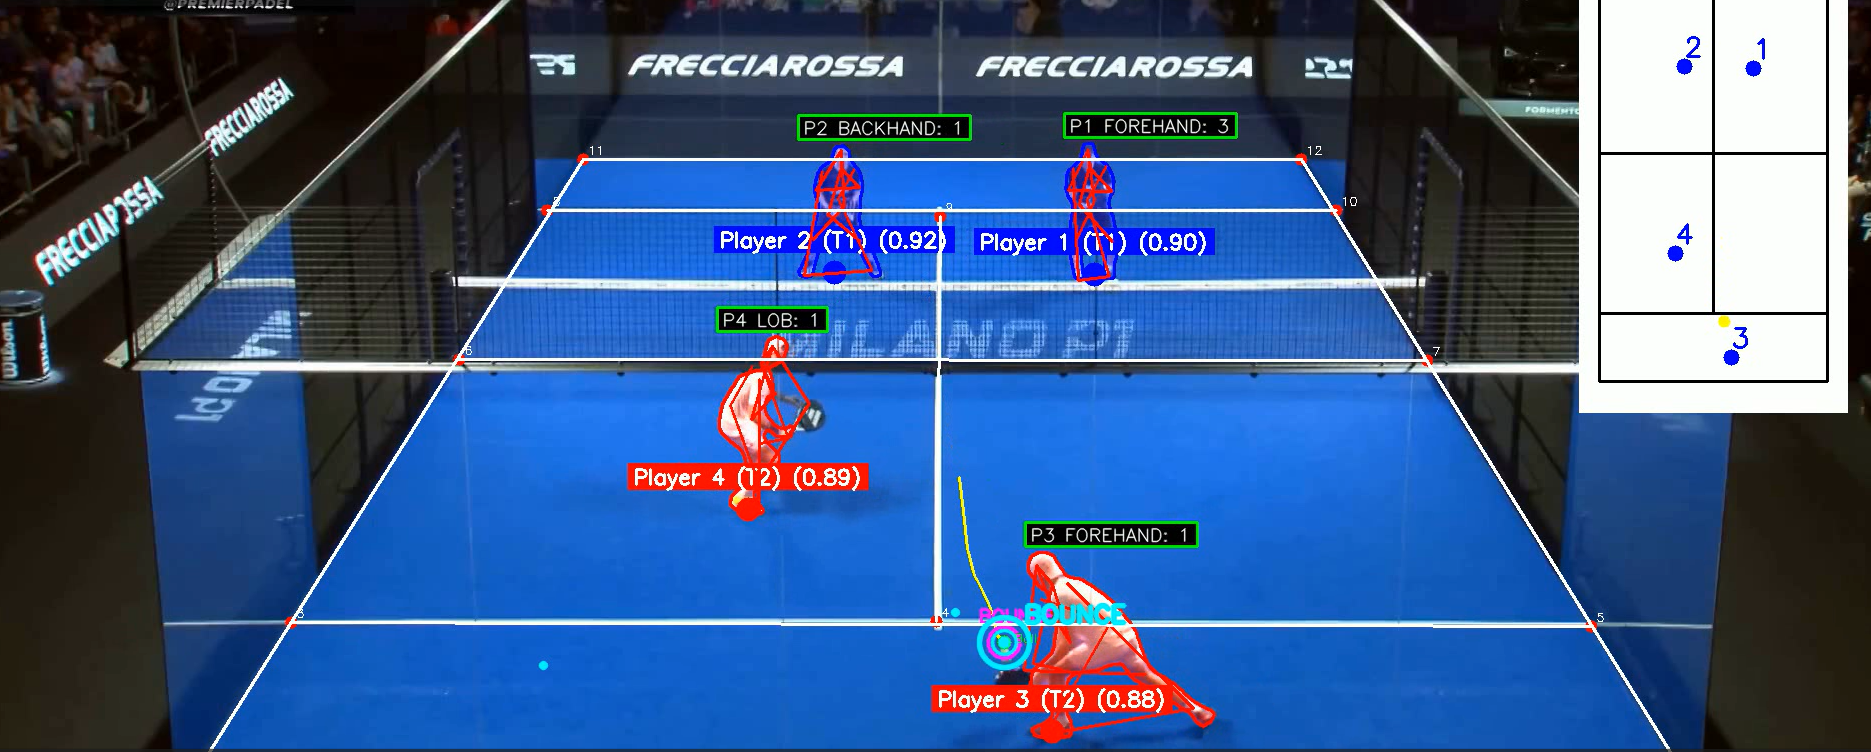
\includegraphics[width=0.85\textwidth]{figures/bounce_detection.png}
    \caption{Détection automatique d’un rebond à partir de l’analyse de la trajectoire de la balle.}
    \label{fig:bounce_detection}
\end{figure}
Pour être validé comme un véritable rebond et non comme un artefact de
prédiction, un pic détecté doit satisfaire deux critères
complémentaires~:
 
\begin{itemize}[leftmargin=*, itemsep=4pt]
 
    \item \textbf{Proéminence minimale}~: le pic doit se détacher de son
    voisinage immédiat d'au moins \textbf{4 pixels} de proéminence
    (\textit{prominence}). Ce seuil permet d'éliminer les faux maxima
    générés par les micro-oscillations résiduelles du signal de
    prédiction, qui peuvent faire trembler la position détectée de un à
    deux pixels d'une trame à l'autre sans correspondre à un événement
    physique réel.
 
    \item \textbf{Intervalle temporel minimal}~: deux rebonds consécutifs
    doivent être séparés d'au moins \textbf{0{,}45 seconde}, afin
    d'éviter les détections multiples issues d'un même contact avec le
    sol.
 
\end{itemize}
 
Cette double contrainte --- proéminence et distance temporelle --- confère
à la détection des rebonds une robustesse notable face au bruit
algorithmique inhérent aux prédictions par réseau de neurones.
 
\subsection{Sorties finales du module BallTracker}

Le module \textit{BallTracker} produit en sortie les indicateurs analytiques suivants :

\begin{itemize}
    \item La trajectoire spatio-temporelle complète de la balle, représentée par les coordonnées $(X, Y)$, le temps $t$ ainsi que l’état de visibilité.
    
    \item Les instants et positions des rebonds validés après le processus de filtrage et d’analyse de proéminence.
    
    \item La vitesse instantanée de la balle, estimée par différentiation temporelle des segments de trajectoire filtrés.
    
\end{itemize}
\begin{figure}[H]
    \centering
    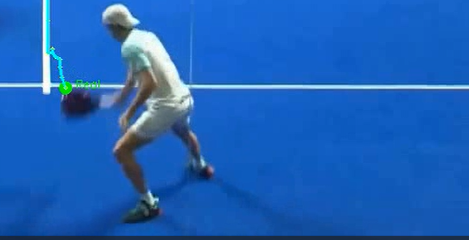
\includegraphics[width=0.32\textwidth]{figures/frame1.png}
    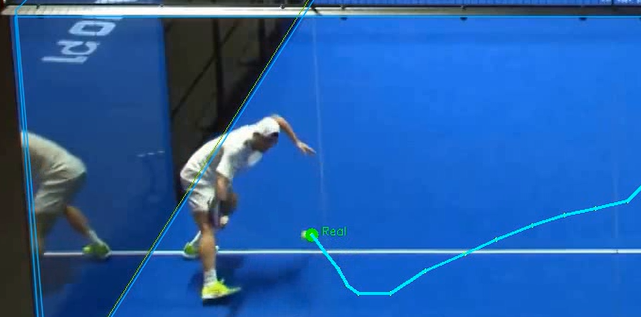
\includegraphics[width=0.32\textwidth]{figures/frame2.png}
    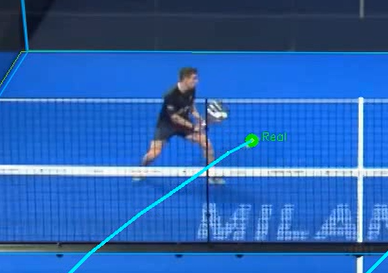
\includegraphics[width=0.32\textwidth]{figures/frame3.png}
    \caption{Illustrations de la position de la balle à différents instants.}
    \label{fig:ball_sequence}
\end{figure}
\subsubsection{Métriques d'évaluation et performances}

L'évaluation quantitative du système de suivi de la balle a été réalisée sur notre base de données de test à l'aide de deux métriques académiques de référence :

\begin{enumerate}
    \item \textbf{PCK@5px (Percentage of Correct Keypoints) :} Pourcentage de prédictions dont la distance euclidienne à la vérité terrain est inférieure ou égale à $5$~pixels.
    \item \textbf{RMSE (Root Mean Squared Error) :} Erreur quadratique moyenne globale en pixels sur l'ensemble de la trajectoire.
\end{enumerate}

Afin de mesurer l'impact de notre chaîne de post-traitement physique et géométrique, nous comparons les performances du modèle \textbf{TrackNet brut} avec notre \textbf{pipeline de suivi robuste} :

\begin{table}[h]
    \centering
    \caption{Comparaison des performances avant et après post-traitement}
    \label{tab:perf_posttraitement}

    \begin{tabular}{lcc}
        \toprule
        \textbf{Configuration} & \textbf{PCK @ 5px ($\uparrow$)} & \textbf{RMSE (pixels) ($\downarrow$)} \\
        \midrule
        \textbf{TrackNet (Brut)} & 86,5 \% & 4,82 px \\
        
        \textbf{Tracknet + les filtres} & \textbf{96,2 \%} & \textbf{1,78 px} \\
        \bottomrule
    \end{tabular}
\end{table}

\textbf{Analyse des résultats :} L'introduction du filtrage robuste permet un gain de \textbf{+9,7 \%} sur le PCK et une division par plus de 2,5 de l'erreur moyenne de trajectoire (RMSE passant de 4,82 à 1,78 pixels). Cette amélioration s'explique par l'élimination systématique des reflets vitrés par le filtre de vitesse et de marge, couplée à la reconstruction fluide des trajectoires d'occlusion par l'interpolation parabolique.

\subsection{Précision, rappel et score F1}

Ces métriques évaluent la capacité du réseau à détecter la présence de la balle sans générer de faux positifs.

\begin{table}[h]
    \centering
    \caption{Comparaison des performances des modèles TrackNet}
    \label{tab:perf_tracknet}
    \vspace{0.5em}
    \begin{tabular}{lccc}
        \toprule
        \textbf{Modèle} & \textbf{Précision} & \textbf{Rappel (Recall)} & \textbf{Score F1} \\
        \midrule
        \textbf{TrackNet (V1)} & 99,7 \% & 97,3 \% & 98,5 \% \\
        \textbf{TrackNetV2}    & 99,6 \% & 94,5 \% & 97,0 \% \\
        \textbf{GridTrackNet}  & 96,6 \% & 93,9 \% & 95,3 \% \\
        \textbf{TrackNetV3}    & 97,8 \%& 99,3 \% & 98,6 \% \\
        \textbf{TrackNetV4}    & 99,6 \% & 92,2 \% & 95,8 \% \\
        \textbf{TrackNetV5}    & 99,2 \% & 98,0 \% & 98,6 \% \\
        \bottomrule
    \end{tabular}
\end{table}

\subsection{Perspectives d'amélioration}

Pour les futures itérations du système, deux axes principaux d’amélioration sont envisagés :

\begin{itemize}
    \item \textbf{Estimation du fond (\textit{Background Estimation}) :} intégrer une image médiane du terrain comme donnée auxiliaire afin d’aider le modèle à distinguer la balle des distractions visuelles telles que les spectateurs ou les panneaux publicitaires.
    
    \item \textbf{Reconstruction 3D :} exploiter les trajectoires 2D détectées afin de reconstruire une représentation tridimensionnelle de la balle, permettant une analyse plus précise de la hauteur et de la vitesse indépendamment de la perspective de la caméra.
\end{itemize}
 
% ------------------------------------------------------------------
\subsection{Synthèse}
\label{subsec:synthesis}
% ------------------------------------------------------------------
 
Le module de suivi de balle repose sur une architecture hybride
combinant la puissance de représentation des réseaux convolutifs
temporels avec une chaîne de post-traitement physiquement informée.
L'intégration de TrackNet pour la génération de heatmaps, couplée à
l'inférence de visibilité, à l'ensemble temporel et au filtrage
multi-étapes, permet d'obtenir une trajectoire de balle précise, continue
et robuste, même dans des conditions visuelles difficiles telles que les
occlusions par les joueurs, les réflexions sur parois vitrées ou les
passages hors-champ. Ces caractéristiques en font un composant central
et fiable du système d'analyse sportive développé dans ce projet.

% ─────────────────────────────────────────────────────────────
\section{Suivi des joueurs}
% ─────────────────────────────────────────────────────────────
 
\subsection{Vue d'ensemble et positionnement dans le pipeline}
 
Le suivi des joueurs produit, à chaque frame, une représentation stable
de la position et de l'identité des quatre joueurs.
Cette stabilité est indispensable aux analyses aval : sans identifiants
persistants, il est impossible de calculer des trajectoires, d'attribuer
des frappes ou de distinguer les deux équipes.
 
Le module adopte une architecture en pipeline séquentiel, de la vidéo
brute jusqu'à la représentation structurée des joueurs, dont les
étapes sont décrites dans les sections suivantes.

 \begin{figure}[H]
    \centering
    \maybeincludegraphics[width=0.9\textwidth]{images_chap2/pipeline_joueurs.png}
    \caption{Pipeline de suivi des joueurs et modules d'identification des équipes.}
    \label{fig:pipeline_joueurs}
\end{figure}
% ─────────────────────────────────────────────────────────────
\subsection{Conversion BGR \texorpdfstring{$\rightarrow$}{->} RGB}
 
Avant toute opération de détection, chaque frame est convertie de
l'espace colorimétrique BGR (format natif d'OpenCV) vers RGB.
Cette conversion est requise car YOLO26 a été entraîné sur des images
en format RGB ; l'omettre introduirait un décalage colorimétrique
systématique dégradant les performances de détection et la cohérence
des descripteurs d'apparence extraits en aval.
 
% ─────────────────────────────────────────────────────────────
\subsection{Détection par YOLO26 fine-tuné}
 
\subsubsection{Choix du modèle YOLO26}
 
Le choix de YOLO26 résulte d'une comparaison entre plusieurs
architectures de détection.
Les modèles de petite taille (nano, small) offrent une vitesse
supérieure mais une précision insuffisante pour des silhouettes filmées
à 15--20\,m de hauteur.
Les modèles larges sont trop coûteux pour un déploiement en temps réel.
L'architecture medium constitue le meilleur compromis
précision/vitesse.
Par rapport aux détecteurs génériques, YOLO26 bénéficie d'un
fine-tuning spécifique sur des images de padel en vue aérienne
(26\textsuperscript{ème} cycle d'entraînement), lui conférant une
robustesse accrue aux silhouettes de faible résolution, aux angles de
vue atypiques et aux occlusions fréquentes entre joueurs.
 
% À insérer dans votre préambule (avant \begin{document}) si ce n'est pas déjà fait :
% \usepackage{tabularx}
% \usepackage{booktabs}

\subsubsection{Paramètres d'inférence}

\begin{table}[h]
    \centering
    \caption{Paramètres d'inférence du détecteur YOLO pour la localisation des joueurs}
    \vspace{0.5em}
    \begin{tabular}{l c p{6.5cm}}
        \toprule
        \textbf{Paramètre} & \textbf{Valeur} & \textbf{Objectif / Justification} \\
        \midrule
        \textbf{Seuil de confiance}  & 0,5 & Élimination des détections ambiguës et faux positifs \\
        \textbf{Seuil IoU (NMS)}     & 0,7 & Suppression des détections redondantes (joueur unique) \\
        \textbf{Résolution d'entrée} & 1280 px & Lisibilité des silhouettes filmées en vue aérienne \\
        \textbf{Classe cible}        & Personne & Restriction exclusive à la détection humaine \\
        \bottomrule
    \end{tabular}
    \label{tab:yolo_params}
\end{table}
 
La résolution de 1280\,px a été retenue pour préserver la lisibilité des
silhouettes filmées à 15--20\,m de hauteur : à plus basse résolution, ces
cibles de faible taille apparente deviennent difficiles à localiser de
manière fiable.
 
\subsubsection{Traitement en lot}
 
Les images sont regroupées en lots de quatre pour une seule passe
\textit{forward}, atteignant un débit environ 3,5$\times$ supérieur
au traitement image par image.
Le dernier lot incomplet en fin de vidéo est géré explicitement.
 
% ─────────────────────────────────────────────────────────────
\begin{figure}[H]
    \centering
    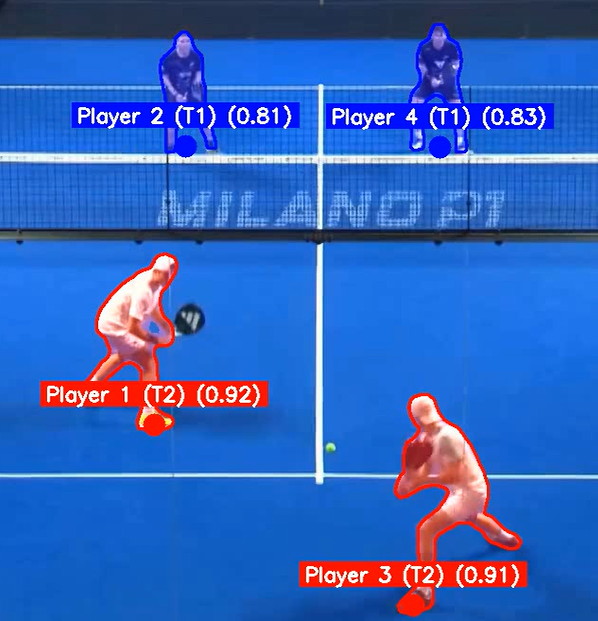
\includegraphics[width=0.79\textwidth]{figures/player_detection_result.png}
    \caption{Résultat du module de détection des joueurs. Chaque joueur est détecté par le modèle YOLO et associé à une équipe (T1 ou T2) ainsi qu'à un score de confiance. Les masques de segmentation permettent une localisation précise des joueurs sur le terrain.}
    \label{fig:player_detection_result}
\end{figure}
\subsection{Filtrage spatial par zone polygonale}
 
\subsubsection{Définition du polygone de terrain}
 
La détection brute génère des faux positifs extérieurs au terrain
(spectateurs, arbitres, cameramen).
Un filtre géométrique appliqué en sortie du détecteur les élimine.
Le terrain est modélisé par 12 points clés définis à la calibration ;
le polygone de filtrage est délimité par les quatre coins extérieurs
\textbf{k1}, \textbf{k2}, \textbf{k12} et \textbf{k11}.

\begin{figure}[H]
    \centering
    \maybeincludegraphics[width=0.9\textwidth]{images_chap2/figure_terrain (1).png}
    \caption{Représentation schématique du terrain de padel avec la zone de filtrage polygonale.}
    \label{fig:terrain_filtrage}
\end{figure}
 
 
\subsubsection{Test d'appartenance à la zone de jeu}
 
L'appartenance est déterminée par un test point-dans-polygone
(\textit{ray-casting}) appliqué au centre-bas de chaque boîte
englobante (point correspondant aux pieds du joueur).
Seules les détections dont le point au sol est à l'intérieur du
quadrilatère sont conservées~--- en pratique, les quatre joueurs
actifs par image.
 
% ─────────────────────────────────────────────────────────────
\subsubsection{Association et suivi : algorithme d’identité stable}

Contrairement aux approches de suivi classiques telles que \textit{ByteTrack}, qui peuvent engendrer des dérives ou des permutations d’identifiants (\textit{ID switches}) lors d’occlusions prolongées ou de croisements à proximité du filet, la stratégie adoptée dans ce module repose sur une identité verrouillée. Une fois les quatre identifiants de joueurs attribués durant la phase d’initialisation, ils demeurent constants tout au long de la séquence vidéo.

\paragraph{Initialisation et assignation des équipes}

La phase d’initialisation est déclenchée de manière déterministe dès que le détecteur observe exactement quatre joueurs simultanément à l’intérieur du polygone représentant le terrain. Les détections sont alors triées selon leur coordonnée verticale $y$ croissante (du haut vers le bas de l’image, ce qui correspond à l’éloignement de la caméra). Les identifiants stables de 1 à 4 sont ensuite attribués définitivement.

L’appartenance à une équipe est déduite directement de cette organisation spatiale lors de la première image valide :

\begin{itemize}
    \item \textbf{Équipe A (Team 1)} : composée des joueurs 1 et 2, correspondant aux deux plus faibles valeurs de $y$, situés dans la moitié supérieure de l’image.
    \item \textbf{Équipe B (Team 2)} : composée des joueurs 3 et 4, correspondant aux deux plus grandes valeurs de $y$, situés dans la moitié inférieure de l’image.
\end{itemize}

Cette stratégie d’initialisation élimine l’instabilité liée à un regroupement (\textit{clustering}) initial et garantit des statistiques d’équipe cohérentes dès les premières images.

\paragraph{Extraction du descripteur d’apparence}

Afin de caractériser visuellement chaque joueur, le système extrait un descripteur de couleur RGB calculé sur les 40\,\% supérieurs de la boîte englobante, correspondant principalement au torse et au maillot. Pour réduire le bruit lié aux plis du tissu et aux variations de texture, un filtre gaussien bidimensionnel de taille $5 \times 5$ est appliqué à la région extraite avant le calcul de la moyenne des canaux :

\[
e = \frac{1}{|\Omega|} \sum_{(r,g,b)\in\Omega}(r,g,b)
\tag{2.4}
\]

où $\Omega$ désigne l’ensemble des pixels de la région considérée.

Le vecteur tridimensionnel
\[
e = [R_{\text{moy}}, G_{\text{moy}}, B_{\text{moy}}]
\]
constitue une signature d’apparence légère permettant de différencier les joueurs, notamment lors des croisements rapprochés.

\paragraph{Prédiction cinématique}

Avant l’étape d’association temporelle, la position future de chaque piste active est estimée par extrapolation linéaire en ajoutant à la position courante une vitesse lissée par une moyenne mobile exponentielle (EMA) avec $\alpha_v = 0{,}5$ :

\[
\hat{b}_{t+1} = b_t + v_t
\tag{2.5}
\]

La vitesse instantanée $v_{\text{inst}}$ est calculée à partir de la différence entre les centres courant et précédent de la boîte englobante. Afin de garantir la cohérence physique du mouvement, le système vérifie que le centre de la boîte prédite $\hat{b}_{t+1}$ demeure à l’intérieur du polygone du terrain. Si ce point sort des limites, la vitesse de la piste est immédiatement réinitialisée à zéro et la prédiction est figée sur la dernière position valide, évitant ainsi toute dérive.

\paragraph{Matrice de coûts et algorithme Hongrois}

L’association entre les pistes actives prédites et les nouvelles détections de l’image courante est formulée comme un problème d’affectation linéaire optimale. Le coût d’association $C(r,c)$ entre une piste $r$ et une détection $c$ est défini par :

\[
C(r,c)=
\begin{cases}
10\,000, & \text{si } d_{\text{spatial}} > 300 \text{ px} \\
d_{\text{spatial}} + 200 \cdot d_{\text{couleur}} + 5 \cdot missed_r, & \text{sinon}
\end{cases}
\tag{2.6}
\]

où :

\begin{itemize}
    \item $d_{\text{spatial}} = \|\hat{c}_r - c_c\|_2$ est la distance euclidienne (en pixels) entre le centre prédit $\hat{c}_r$ de la piste $r$ et le centre $c_c$ de la détection $c$.
    \item $d_{\text{couleur}} = \dfrac{\|e_r - e_c\|_2}{255}$ est la distance euclidienne normalisée entre les signatures colorimétriques.
    \item $missed_r$ représente le nombre d’images consécutives durant lesquelles la piste $r$ n’a pas été associée à une détection.
\end{itemize}

Le seuil géométrique strict de 300 pixels agit comme une étape de \textit{gating}, attribuant un coût prohibitif de 10\,000 à toute association jugée physiquement impossible. Le coefficient 200 appliqué à la distance colorimétrique confère un poids important à l’identité visuelle du maillot.

La résolution globale de cette matrice de coûts est assurée par l’algorithme de Kuhn-Munkres, également appelé algorithme Hongrois, dont la complexité est de $\mathcal{O}(n^3)$.

\paragraph{Mise à jour des pistes par moyenne exponentielle mobile}

Une fois l’association résolue, les états des pistes ayant trouvé une correspondance sont mis à jour comme suit :

\begin{itemize}
    \item \textbf{Vitesse :} si le joueur a été absent durant plus de cinq images ($missed > 5$), sa vitesse est réinitialisée à zéro. Sinon, elle est mise à jour à l’aide d’une EMA réactive ($\alpha_v = 0{,}5$) :
    \[
    v_t \leftarrow 0.5 \cdot v_{\text{inst}} + 0.5 \cdot v_{t-1}
    \]

    \item \textbf{Apparence :} le descripteur colorimétrique est actualisé à l’aide d’une EMA à mémoire longue ($\alpha_c = 0{,}1$), permettant de s’adapter progressivement aux variations d’éclairage :
    \[
    e_t \leftarrow 0.1 \cdot e_{\text{det}} + 0.9 \cdot e_{t-1}
    \]
\end{itemize}

Cette combinaison entre prédiction cinématique, descripteur d’apparence et association globale garantit un suivi robuste et stable des quatre joueurs sur l’ensemble de la vidéo, tout en éliminant efficacement les permutations d’identifiants.

% ─────────────────────────────────────────────────────────────
\subsection{Robustesse aux situations critiques}
 
\subsubsection{Occlusion et croisement de joueurs}
 
Lors d'un croisement, les boîtes englobantes deviennent
quasi-identiques spatialement.
L'algorithme Hongrois minimise le coût global de l'affectation plutôt
que paire par paire, identifiant la combinaison optimale.
Le descripteur colorimétrique joue alors un rôle discriminant essentiel
entre joueurs d'équipes différentes.
 
\subsubsection{Disparition temporaire d'un joueur}
 
Un joueur absent (sortie de terrain, occlusion totale, chute) voit son
identifiant maintenu pendant 90 frames ($\approx$3\,s à 30\,fps), sa
position extrapolée à partir de sa dernière vitesse.
Au-delà de 5 frames d'absence, la vitesse est réinitialisée à zéro
pour éviter une extrapolation divergente.
Passé le délai de 90 frames sans réassociation, la piste est supprimée
et un nouveau cycle d'initialisation est attendu.
La pénalité progressive garantit une récupération rapide dès la
réapparition du joueur.
 
\subsubsection{Nombre insuffisant de joueurs détectés}
 
En phase d'initialisation, si le nombre de détections est différent de
quatre, le système diffère d'une frame sans produire de sortie.
En phase de suivi active, les pistes établies sont maintenues par le
mécanisme de persistance prédictive.
 
% ─────────────────────────────────────────────────────────────
\subsection{Extension par segmentation au niveau pixel}
 
Une variante intègre SAM2 (\textit{Segment Anything Model 2}) en
complément de YOLO26 : les boîtes englobantes servent de
\textit{prompts} au modèle de segmentation, qui produit des masques
pixel-level.
Cette extension améliore la précision de localisation pour des analyses
de posture ou de gestuelle, au prix d'un coût computationnel nettement
plus élevé, réservé aux scénarios où la précision prime sur le temps
réel.
 
% ─────────────────────────────────────────────────────────────
\subsection{Synthèse}
Le module de suivi des joueurs repose sur un enchaînement séquentiel de cinq étapes clés :
\begin{enumerate}
    \item \textbf{Prétraitement colorimétrique :} La conversion de l'espace $BGR \rightarrow RGB$ afin d'éviter tout décalage colorimétrique lors de l'inférence et de l'extraction des signatures.
    \item \textbf{Détection et filtrage spatial :} L'inférence par le modèle YOLO26 fine-tuné à haute résolution ($1280$~px) couplée à un filtrage géométrique par lancer de rayon (\textit{ray-casting}) dans le polygone convexe défini par les limites du court.
    \item \textbf{Partitionnement géographique initial :} L'attribution déterministe des équipes lors du premier frame valide (moitié supérieure pour l'équipe A, moitié inférieure pour l'équipe B), évitant l'instabilité des méthodes de clustering non supervisées au démarrage.
    \item \textbf{Association globale optimale :} L'appariement des pistes et des détections via l'algorithme Hongrois, en minimisant une matrice de coûts composite associant distance euclidienne spatiale, distance colorimétrique RGB du torse et pénalité de disparition temporelle.
    \item \textbf{Gestion robuste des occlusions :} La persistance prédictive des pistes par extrapolation cinématique et maintien de la mémoire couleur (\textit{slot-holding}) jusqu'à $90$~frames (environ $3$~secondes à $30$~fps).
\end{enumerate}

Cet ensemble de mécanismes garantit un suivi stable et continu sur toute la durée du match, ce qui constitue une condition \textit{sine qua non} pour la fiabilité des modules d'analyse statistique situés en aval du pipeline.


\section{Modèle d'estimation des points clés des joueurs}

\subsection{Introduction}

La détection des joueurs par boîtes englobantes permet uniquement de localiser les athlètes dans l’image. Cependant, cette représentation reste insuffisante pour analyser précisément les mouvements, les postures et les gestes techniques durant un match de padel.

Afin d’obtenir une compréhension plus détaillée des actions des joueurs, la plateforme SmartPlayAI intègre un module d’estimation de pose basé sur YOLOv8-Pose. Ce modèle permet d’extraire automatiquement les points clés squelettiques des joueurs à partir des séquences vidéo et de représenter leur posture en temps réel.

\subsection{Architecture du modèle YOLOv8-Pose}

Le modèle utilisé repose sur l’architecture YOLOv8-Pose, capable d’effectuer simultanément la détection des joueurs et l’estimation de leurs points clés dans une seule passe d’inférence. Cette approche améliore considérablement les performances temps réel.

L’architecture comprend trois composants principaux :

\begin{itemize}
    \item \textbf{Backbone (CSPDarknet)} : extraction des caractéristiques visuelles profondes ;
    \item \textbf{Neck (PAN-FPN)} : fusion multi-échelles des cartes de caractéristiques ;
    \item \textbf{Pose Head} : prédiction des boîtes englobantes et des points clés corporels.
\end{itemize}

\begin{table}[H]
\centering
\caption{Composants principaux de YOLOv8-Pose}
\label{tab:composants_yolopose}
\begin{tabular}{|c|c|}
\hline
\textbf{Composant} & \textbf{Rôle} \\
\hline
Backbone & Extraction des caractéristiques visuelles \\
\hline
Neck & Fusion multi-échelles \\
\hline
Pose Head & Prédiction des keypoints et des boîtes \\
\hline
\end{tabular}
\end{table}

\subsection{Estimation des points clés}

Pour chaque joueur détecté, le modèle prédit les coordonnées des articulations corporelles selon la convention COCO à 17 points clés. Chaque articulation est représentée par :

\begin{equation}
p_i = (x_i, y_i, c_i)
\end{equation}

où :
\begin{itemize}
    \item $x_i$ et $y_i$ représentent les coordonnées du point clé ;
    \item $c_i$ correspond au score de confiance associé.
\end{itemize}

Les points clés couvrent les principales régions anatomiques : tête, épaules, coudes, poignets, hanches, genoux et chevilles.

\subsection{Pipeline d’inférence}

Le traitement d’une trame vidéo commence par une phase de prétraitement et de normalisation de l’image d’entrée. Les caractéristiques visuelles profondes sont ensuite extraites à l’aide du Backbone, puis fusionnées à différentes échelles grâce au module Neck afin d’améliorer la détection des structures anatomiques. Le modèle réalise ensuite la détection des joueurs ainsi que l’estimation simultanée des points clés corporels. Les détections redondantes sont supprimées à l’aide de l’algorithme NMS (\textit{Non-Maximum Suppression}), avant de générer les squelettes associés aux joueurs détectés. Cette pipeline permet d’obtenir en temps réel une représentation squelettique complète et précise des joueurs présents sur le terrain.

\subsection{Adaptation au contexte du padel}

L’estimation de pose dans le padel reste complexe à cause des mouvements rapides, des occultations et des vues aériennes. Afin d’améliorer les performances, un fine-tuning du modèle a été réalisé sur des séquences réelles de matchs de padel.

Cette adaptation permet d’augmenter la précision des articulations détectées et d’améliorer la robustesse du système dans des scènes sportives dynamiques.

\subsection{Applications dans SmartPlayAI}

Les points clés extraits sont exploités dans plusieurs modules analytiques :

\begin{table}[H]
\centering
\caption{Applications des points clés dans SmartPlayAI}
\label{tab:applications_keypoints}
\begin{tabular}{|c|c|}
\hline
\textbf{Application} & \textbf{Utilité} \\
\hline
Projection géométrique & Position précise des joueurs sur le terrain \\
\hline
Reconnaissance de gestes & Détection des smashs, volées et revers \\
\hline
Analyse biomécanique & Étude des angles articulaires et des mouvements \\
\hline
\end{tabular}
\end{table}

Les données squelettiques permettent ainsi d’enrichir l’analyse tactique et biomécanique des matchs.

\subsection{Conclusion}

Le module YOLOv8-Pose constitue un élément essentiel de SmartPlayAI. Grâce à l’estimation des points clés, le système dépasse la simple détection des joueurs et fournit une analyse avancée des mouvements, des gestes techniques et des comportements tactiques durant les matchs de padel.
% ════════════════════════════════════════════════════════════════════════════
\section{Module d'analyse biomécanique et tactique}
% ════════════════════════════════════════════════════════════════════════════

\subsection{Objectifs et rôle du module}

Le module d'analyse biomécanique et tactique constitue le noyau analytique de la plateforme
SmartPlayAI. Son rôle fondamental est de transformer les coordonnées brutes des joueurs et de
la balle — issues de la chaîne de détection et de suivi vidéo — en un ensemble structuré
d'indicateurs quantitatifs exploitables à des fins d'analyse de la performance sportive.

À partir des positions projetées dans le référentiel métrique du terrain, le module calcule
un ensemble d'indicateurs cinématiques couvrant les déplacements, les vitesses, les
accélérations et les distances parcourues. Ces grandeurs servent ensuite à identifier les
événements de jeu, à caractériser les actions techniques réalisées par les joueurs et à
alimenter un système automatisé de suivi du score.

Ce module assure ainsi la transition entre les données brutes issues de la vision par
ordinateur et les informations à forte valeur ajoutée destinées aux entraîneurs, aux
analystes et aux joueurs. Ses objectifs principaux se déclinent en quatre axes :

\begin{itemize}[leftmargin=1.5em]
  \item Projection et normalisation spatiale des positions détectées dans un référentiel
        métrique standardisé ;
  \item Construction d'un modèle de données temporel enrichi regroupant déplacements,
        vitesses et accélérations à plusieurs granularités temporelles ;
  \item Détection et classification automatique des événements de jeu (frappes, types
        de coups) ;
  \item Suivi automatisé du score conformément aux règles officielles du padel.
\end{itemize}

% ────────────────────────────────────────────────────────────────────────────
\subsection{Architecture générale du pipeline d'analyse}
% ────────────────────────────────────────────────────────────────────────────

Le pipeline d'analyse repose sur une succession d'étapes permettant d'enrichir
progressivement les données extraites de la vidéo. Chaque étape produit une représentation
plus élaborée de l'information, depuis les coordonnées pixel brutes jusqu'à un ensemble
complet d'indicateurs analytiques prêts à l'exportation.

Dans un premier temps, les positions des joueurs et de la balle sont exprimées dans un
référentiel métrique associé au terrain de padel. Ces positions sont ensuite organisées
sous la forme d'une structure de données temporelle permettant de suivre l'évolution de
chaque entité au cours du match. Les données ainsi structurées servent ensuite au calcul
des indicateurs biomécaniques, lesquels alimentent en aval les modules de détection des
frappes, de reconnaissance des types de coups et de mise à jour automatique du score.

Le Tableau~\ref{tab:pipeline_dataanalytics} résume les six étapes séquentielles du pipeline
ainsi que les formats de données produits à chaque niveau de traitement.

\begin{table}[H]
  \centering
  \renewcommand{\arraystretch}{1.3}
  \begin{tabularx}{\textwidth}{L{2.8cm} X L{4cm}}
    \rowcolor{tablehead}
    \textcolor{white}{\textbf{Étape}} &
    \textcolor{white}{\textbf{Description}} &
    \textcolor{white}{\textbf{Format de sortie}} \\
    \rowcolor{rowalt}
    Acquisition   & Réception des positions des joueurs et de la balle à chaque trame vidéo
                  & Coordonnées pixel $(p_x, p_y)$ \\
    Projection    & Transformation homographique et conversion en unités métriques
                  & Coordonnées métriques $(x_m, y_m)$ \\
    \rowcolor{rowalt}
    Accumulation  & Construction d'un enregistrement par trame et empilement en série temporelle
                  & Liste de $N$ enregistrements \\
    Enrichissement & Calcul des déplacements, vitesses et accélérations sur 4 intervalles temporels
                  & DataFrame de 179 colonnes \\
    \rowcolor{rowalt}
    Analyse événementielle & Détection des frappes, classification des coups, suivi du score
                  & Événements horodatés + score \\
    Export        & Sérialisation en fichier CSV pour exploitation post-match
                  & Fichier \texttt{.csv} ($\approx 3{,}2$\,Mo/match) \\
  \end{tabularx}
  \caption{Flux de traitement du module DataAnalytics}
  \label{tab:pipeline_dataanalytics}
\end{table}

% ────────────────────────────────────────────────────────────────────────────
\subsection{Acquisition et structuration des données}
% ────────────────────────────────────────────────────────────────────────────

\subsubsection{Référentiel spatial du terrain}

L'ensemble des calculs est réalisé dans un système de coordonnées métrique centré sur le
filet. Ce choix garantit une symétrie naturelle entre les deux demi-terrains et simplifie
les comparaisons entre équipes. Les dimensions réglementaires définies par la Fédération
Internationale de Padel (FIP) fixent les bornes du référentiel :

\begin{itemize}[leftmargin=1.5em]
  \item L'axe $X$ (largeur du terrain) s'étend de $-5$\,m à $+5$\,m ;
  \item L'axe $Y$ (longueur du terrain) s'étend de $-10$\,m à $+10$\,m.
\end{itemize}

Le Tableau~\ref{tab:constantes_fip} récapitule les constantes réglementaires FIP utilisées
pour définir les bornes du référentiel.

\begin{table}[H]
  \centering
  \renewcommand{\arraystretch}{1.3}
  \begin{tabularx}{\textwidth}{L{4.4cm} C{2cm} C{1.5cm} X}
    \rowcolor{tablehead}
    \textcolor{white}{\textbf{Constante}} &
    \textcolor{white}{\textbf{Valeur}} &
    \textcolor{white}{\textbf{Axe}} &
    \textcolor{white}{\textbf{Description}} \\
    \rowcolor{rowalt}
    \texttt{base\_line}         & 10\,m & $X$ & Demi-largeur du terrain \\
    \texttt{side\_line}         & 20\,m & $Y$ & Longueur totale du terrain \\
    \rowcolor{rowalt}
    \texttt{service\_side\_line} & 3\,m  & $Y$ & Distance ligne de service au fond de court \\
    \texttt{net\_side\_line}    & 10\,m & $Y$ & Distance filet au fond de court \\
  \end{tabularx}
  \caption{Constantes réglementaires FIP et bornes du référentiel terrain}
  \label{tab:constantes_fip}
\end{table}

\subsubsection{Projection homographique des positions}

La caméra placée en vue aérienne capture le terrain selon une perspective introduisant des
déformations géométriques. Pour corriger ces distorsions et obtenir des coordonnées métriques
fidèles, une transformation homographique est appliquée — représentation mathématique standard
d'une projection plan-à-plan en vision par ordinateur.

Formellement, un point $\mathbf{p} = (p_x, p_y)^\top$ exprimé en pixels est converti en
coordonnées homogènes $\tilde{\mathbf{p}} = (p_x, p_y, 1)^\top$, puis projeté par la matrice
d'homographie $H \in \mathbb{R}^{3 \times 3}$ calculée lors de l'étalonnage de la caméra :

\begin{equation}
  \tilde{\mathbf{p}}' = H \cdot \tilde{\mathbf{p}}, \qquad
  \mathbf{p}' = \frac{1}{\tilde{p}'_3} \cdot \bigl(\tilde{p}'_1,\, \tilde{p}'_2\bigr)^\top
  \label{eq:homographie}
\end{equation}

La conversion vers le référentiel métrique FIP s'effectue ensuite en soustrayant l'origine
(centre du filet) et en appliquant les facteurs d'échelle correspondant aux dimensions
réglementaires :

\begin{equation}
  x_m = \Delta p_x \cdot \frac{B_{\mathrm{LINE}}}{W_{\mathrm{terrain}}}, \qquad
  y_m = \Delta p_y \cdot \frac{S_{\mathrm{LINE}}}{H_{\mathrm{terrain}}}
  \label{eq:conversion_metrique}
\end{equation}

où $\Delta p_x$ et $\Delta p_y$ désignent les déplacements par rapport à l'origine dans la
mini-carte, et $W_{\mathrm{terrain}}$, $H_{\mathrm{terrain}}$ sont les dimensions en pixels
de cette mini-carte. On obtient ainsi, pour chaque joueur, une position $(x_m, y_m)$
exprimée en mètres dans le référentiel centré sur le filet.

\subsubsection{Structuration temporelle des observations}

À chaque trame vidéo, le système constitue un enregistrement structuré regroupant l'ensemble
des informations spatiales de l'instant considéré. Cet enregistrement comprend : l'indice de
trame (identifiant entier incrémental), la liste des positions des quatre joueurs exprimées en
coordonnées métriques, et la position de la balle (ou une valeur nulle si la balle n'est pas
détectée).

Ces enregistrements sont empilés au fil des trames pour constituer la série temporelle brute
qui alimente l'étape d'enrichissement cinématique. Cette organisation facilite l'analyse
dynamique des comportements individuels et collectifs au cours du match.

% ────────────────────────────────────────────────────────────────────────────
\subsection{Construction du modèle de données analytique}
% ────────────────────────────────────────────────────────────────────────────

L'ensemble des enregistrements accumulés est converti en un tableau de données tabulaire dont
chaque ligne correspond à une trame vidéo. Dans sa forme brute, ce tableau comporte 11 colonnes
de base décrites dans le Tableau~\ref{tab:colonnes_base}.

\begin{table}[H]
  \centering
  \renewcommand{\arraystretch}{1.3}
  \begin{tabularx}{\textwidth}{L{3.5cm} C{2cm} C{2cm} X}
    \rowcolor{tablehead}
    \textcolor{white}{\textbf{Colonne}} &
    \textcolor{white}{\textbf{Type}} &
    \textcolor{white}{\textbf{Unité}} &
    \textcolor{white}{\textbf{Description}} \\
    \rowcolor{rowalt}
    \texttt{frame}                        & entier & — & Indice de trame (0, 1, 2, \ldots) \\
    \texttt{player\{i\}\_x} ($i = 1..4$) & réel   & mètre & Position $X$ du joueur $i$ \\
    \rowcolor{rowalt}
    \texttt{player\{i\}\_y} ($i = 1..4$) & réel   & mètre & Position $Y$ du joueur $i$ \\
    \texttt{ball\_x}                      & réel   & mètre & Position $X$ de la balle \\
    \rowcolor{rowalt}
    \texttt{ball\_y}                      & réel   & mètre & Position $Y$ de la balle \\
  \end{tabularx}
  \caption{Colonnes de base du tableau de données brut}
  \label{tab:colonnes_base}
\end{table}

Chaque trame est associée à un horodatage absolu exprimé en secondes, calculé à partir de
l'indice de trame $n$ et de la cadence d'acquisition $f_s \in \{25, 30\}$ images par
seconde :

\begin{equation}
  t[n] = \frac{n}{f_s}
  \label{eq:horodatage}
\end{equation}

En ce qui concerne la gestion des données manquantes, lors des phases d'occultation (joueur
hors-champ, superposition de silhouettes), la détection peut échouer pour un ou plusieurs
joueurs. Ces absences sont enregistrées comme valeurs nulles puis converties en valeurs
indéfinies (\texttt{NaN}) lors de la construction du tableau. Ces valeurs manquantes sont
propagées de façon cohérente lors du calcul des indicateurs cinématiques, garantissant
qu'aucun artefact numérique n'est introduit dans les séries temporelles.

Enfin, la structure tabulaire unifiée ainsi constituée comporte 179 colonnes au total,
réparties en trois familles : 11 colonnes fixes (indices, horodatages, coordonnées),
4 colonnes temporelles (intervalles $\Delta t_k$) et 164 colonnes cinématiques issues de
l'enrichissement multi-intervalle décrit à la section suivante.

% ────────────────────────────────────────────────────────────────────────────
\subsection{Extraction des indicateurs biomécaniques}
% ────────────────────────────────────────────────────────────────────────────

L'enrichissement cinématique repose sur une stratégie multi-intervalle : les déplacements,
vitesses et accélérations sont calculés simultanément sur quatre fenêtres temporelles
correspondant à $k \in \{1, 2, 3, 4\}$ trames successives. L'intervalle temporel associé à
chaque valeur de $k$ est défini par :

\begin{equation}
  \Delta t_k[n] = t[n] - t[n-k] = \frac{k}{f_s}
  \label{eq:intervalle}
\end{equation}

Le Tableau~\ref{tab:niveaux_lissage} résume les quatre niveaux de lissage et leurs usages
recommandés. Le choix $k = 4$ (fenêtre de 133\,ms) est justifié par le fait que cette durée
correspond au seuil minimal du temps de réaction humain. Elle permet de réduire l'erreur de
bruit de position sans introduire de retard perceptible dans la détection des vrais
changements de direction.

\begin{table}[H]
  \centering
  \renewcommand{\arraystretch}{1.3}
  \begin{tabularx}{\textwidth}{C{1cm} C{2.5cm} C{2cm} X}
    \rowcolor{tablehead}
    \textcolor{white}{\textbf{$k$}} &
    \textcolor{white}{\textbf{$\Delta t_k$ à 30\,fps}} &
    \textcolor{white}{\textbf{Lissage}} &
    \textcolor{white}{\textbf{Usage recommandé}} \\
    \rowcolor{rowalt}
    1 & $\approx 33$\,ms  & Aucun   & Signal de référence ; bruit de détection élevé \\
    2 & $\approx 67$\,ms  & Faible  & Détection des changements dynamiques rapides \\
    \rowcolor{rowalt}
    3 & $\approx 100$\,ms & Modéré  & Analyse des transitions tactiques \\
    4 & $\approx 133$\,ms & Fort    & Recommandé — lissage optimal pour la performance \\
  \end{tabularx}
  \caption{Intervalles temporels et niveaux de lissage associés}
  \label{tab:niveaux_lissage}
\end{table}

\subsubsection{Analyse des déplacements}

Le déplacement entre la trame $n-k$ et la trame $n$ est calculé, pour chaque composante,
par différence arithmétique des positions :

\begin{equation}
  \Delta x_k[n] = x[n] - x[n-k], \qquad \Delta y_k[n] = y[n] - y[n-k]
  \label{eq:deplacement}
\end{equation}

Ces grandeurs sont exprimées en mètres. Pour $k = 4$ à 30\,fps, les plages typiques
observées en match de padel sont comprises entre $-30$\,cm et $+30$\,cm, reflétant les
micro-ajustements posturaux et les déplacements courts caractéristiques de ce sport.

\subsubsection{Analyse des vitesses}

La vitesse instantanée est estimée par différences finies du premier ordre appliquées aux
déplacements. Pour chacune des deux composantes :

\begin{equation}
  V_{x,k}[n] = \frac{\Delta x_k[n]}{\Delta t_k} = \frac{x[n] - x[n-k]}{k/f_s}
  \label{eq:vitesse_x}
\end{equation}

\begin{equation}
  V_{y,k}[n] = \frac{\Delta y_k[n]}{\Delta t_k}
  \label{eq:vitesse_y}
\end{equation}

La vitesse scalaire (norme euclidienne du vecteur vitesse) est définie par :

\begin{equation}
  V_{\mathrm{norm},k}[n] = \sqrt{V_{x,k}[n]^2 + V_{y,k}[n]^2}
  \label{eq:vitesse_norme}
\end{equation}

Le Tableau~\ref{tab:vitesses_padel} présente les plages de vitesse scalaire caractéristiques
observées en match de padel.

\begin{table}[H]
  \centering
  \renewcommand{\arraystretch}{1.3}
  \begin{tabularx}{\textwidth}{X C{3.5cm}}
    \rowcolor{tablehead}
    \textcolor{white}{\textbf{Situation locomotrice}} &
    \textcolor{white}{\textbf{$V_{\mathrm{norm}}$ (m/s)}} \\
    \rowcolor{rowalt}
    Joueur immobile (phase d'attente)    & $0{,}0 - 0{,}3$ \\
    Déplacement latéral (pas chassés)    & $1{,}5 - 3{,}5$ \\
    \rowcolor{rowalt}
    Sprint en direction d'un smash       & $4{,}0 - 6{,}5$ \\
    Vitesse maximale relevée             & $\approx 7{,}0$ \\
  \end{tabularx}
  \caption{Plages de vitesse scalaire caractéristiques observées en match de padel}
  \label{tab:vitesses_padel}
\end{table}

\subsubsection{Analyse des accélérations}

L'accélération est obtenue par différences finies du second ordre appliquées aux vecteurs
vitesse :

\begin{equation}
  A_{x,k}[n] = \frac{V_{x,k}[n] - V_{x,k}[n-k]}{\Delta t_k}
  \label{eq:accel_x}
\end{equation}

\begin{equation}
  A_{y,k}[n] = \frac{V_{y,k}[n] - V_{y,k}[n-k]}{\Delta t_k}
  \label{eq:accel_y}
\end{equation}

L'accélération scalaire correspondante est :

\begin{equation}
  A_{\mathrm{norm},k}[n] = \sqrt{A_{x,k}[n]^2 + A_{y,k}[n]^2}
  \label{eq:accel_norme}
\end{equation}

Le Tableau~\ref{tab:accelerations_padel} répertorie les plages caractéristiques selon les
événements biomécaniques observés en padel.

\begin{table}[H]
  \centering
  \renewcommand{\arraystretch}{1.3}
  \begin{tabularx}{\textwidth}{X C{3.5cm}}
    \rowcolor{tablehead}
    \textcolor{white}{\textbf{Événement biomécanique}} &
    \textcolor{white}{\textbf{$A_{\mathrm{norm}}$ (m/s²)}} \\
    \rowcolor{rowalt}
    Course en régime stabilisé                              & $0{,}0 - 2{,}0$ \\
    Changement de direction                                 & $5{,}0 - 12{,}0$ \\
    \rowcolor{rowalt}
    Départ de sprint                                        & $8{,}0 - 15{,}0$ \\
    Phase de frappe (bras, via points squelettiques)        & $> 20{,}0$ \\
  \end{tabularx}
  \caption{Plages d'accélération scalaire caractéristiques observées en padel}
  \label{tab:accelerations_padel}
\end{table}

\subsubsection{Distance parcourue et intensité de jeu}

La distance inter-trame est calculée avec $k = 1$ (trames consécutives), afin de minimiser
les erreurs de rectification liées aux trajectoires curvilignes :

\begin{equation}
  d[n] = \sqrt{\bigl(x[n] - x[n-1]\bigr)^2 + \bigl(y[n] - y[n-1]\bigr)^2}
  \label{eq:distance_intertrame}
\end{equation}

La distance totale parcourue sur une séquence de $N$ trames s'obtient par sommation
cumulative :

\begin{equation}
  D_{\mathrm{tot}} = \sum_{n=1}^{N} d[n]
  \label{eq:distance_totale}
\end{equation}

Les valeurs typiques observées se situent entre 50 et 200\,m pour un échange complet, selon
l'intensité et la durée du rallye. Combinée aux vitesses et aux accélérations, cette métrique
permet d'évaluer la charge physique associée aux différentes phases de jeu.

% ────────────────────────────────────────────────────────────────────────────
\subsection{Analyse événementielle des échanges}
% ────────────────────────────────────────────────────────────────────────────

\subsubsection{Détection des frappes}

La détection d'un impact raquette-balle repose sur une hypothèse physique fondamentale : une
frappe se traduit par une discontinuité brutale du vecteur vitesse de la balle, caractérisée
soit par un changement de direction marqué, soit par une variation soudaine de son énergie
cinétique. L'algorithme opère en deux phases successives.

Lors de la première phase, les vitesses pré- et post-impact sont estimées sur une fenêtre
glissante de $W = 5$ trames de part et d'autre du moment analysé :

\begin{equation}
  \bar{V}^{\mathrm{pre}}_x = \frac{1}{W-1} \sum_{i=t-W}^{t-2} \bigl(x[i+1] - x[i]\bigr)
  \label{eq:vitesse_pre}
\end{equation}

et de façon symétrique pour la composante $y$ et la fenêtre post-impact. Lors de la seconde
phase, un impact est validé si au moins l'un des deux critères suivants est vérifié :

\begin{itemize}[leftmargin=1.5em]
  \item \textbf{Changement de direction :} le cosinus de l'angle entre les vecteurs vitesse
        pré- et post-impact est négatif, correspondant à une inversion de trajectoire
        supérieure à 90° :
        \begin{equation}
          \cos\theta = \frac{\vec{V}_{\mathrm{pre}} \cdot \vec{V}_{\mathrm{post}}}%
                            {\|\vec{V}_{\mathrm{pre}}\| \cdot \|\vec{V}_{\mathrm{post}}\|}
                      < 0
          \label{eq:cos_theta}
        \end{equation}
  \item \textbf{Accélération brutale :} le rapport des normes de vitesse post-impact et
        pré-impact dépasse un seuil $\alpha > 1$ :
        \begin{equation}
          \frac{\|\vec{V}_{\mathrm{post}}\|}{\|\vec{V}_{\mathrm{pre}}\|} > \alpha, \qquad
          \alpha = 1{,}6
          \label{eq:seuil_acceleration}
        \end{equation}
\end{itemize}

Un mécanisme de période réfractaire interdit la détection d'un second impact dans un
intervalle minimal de $\approx 0{,}83$\,s à 30\,fps (25 trames), éliminant ainsi les faux
positifs liés aux micro-oscillations de détection. Le Tableau~\ref{tab:params_detecteur}
récapitule les paramètres de configuration du détecteur.

\begin{table}[H]
  \centering
  \renewcommand{\arraystretch}{1.3}
  \begin{tabularx}{\textwidth}{L{5cm} C{3cm} X}
    \rowcolor{tablehead}
    \textcolor{white}{\textbf{Paramètre}} &
    \textcolor{white}{\textbf{Valeur}} &
    \textcolor{white}{\textbf{Interprétation physique}} \\
    \rowcolor{rowalt}
    Seuil de proximité balle-joueur & 180\,px   & $\approx 1{,}5$\,m en vue drone (1080p) \\
    Période réfractaire individuelle & 25 trames & $\approx 0{,}83$\,s à 30\,fps \\
    \rowcolor{rowalt}
    Seuil d'inversion directionnelle & $\cos\theta < 0$ & Angle d'inversion $> 90°$ \\
    Seuil d'accélération $\alpha$    & 1,6       & Rapport vitesse post/pré-impact \\
    \rowcolor{rowalt}
    Vitesse minimale de la balle     & 12\,px/trame & Filtrage des micro-tremblements \\
    Période réfractaire globale      & 12 trames & $\approx 0{,}4$\,s entre deux coups \\
  \end{tabularx}
  \caption{Paramètres de configuration du détecteur de frappes}
  \label{tab:params_detecteur}
\end{table}

\subsubsection{Attribution des frappes aux joueurs}

Une fois un impact détecté, il est attribué au joueur le plus vraisemblablement responsable
de la frappe. Cette attribution repose sur une distance effective combinant deux mesures de
proximité entre la balle et chaque joueur :

\begin{equation}
  d_{\mathrm{eff}} = \min\bigl(d_{\mathrm{centre}},\; d_{\mathrm{poignet}}\bigr)
  \label{eq:distance_effective}
\end{equation}

où $d_{\mathrm{centre}}$ désigne la distance entre la balle et le centre de la boîte de
détection du joueur, et $d_{\mathrm{poignet}}$ la distance entre la balle et le poignet du
joueur (lorsque les points squelettiques articulaires sont disponibles). L'utilisation de la
position du poignet améliore significativement la précision d'attribution lors des phases de
smash.

\subsubsection{Classification des types de coups}

Chaque coup détecté est classifié en l'une des six catégories techniques du padel :
Smash, Bandeja, Coup droit (\textit{Forehand}), Revers (\textit{Backhand}), Volley et
Service. La classification s'appuie sur l'analyse d'une fenêtre temporelle de
$\pm 10$ trames ($\approx 700$\,ms à 30\,fps) centrée sur le point d'impact. Le vecteur
de caractéristiques extrait comprend :

\begin{itemize}[leftmargin=1.5em]
  \item les 21 distances balle-poignet calculées trame par trame dans la fenêtre d'analyse ;
  \item la hauteur relative de la balle par rapport à la tête du joueur frappeur ;
  \item les angles articulaires épaule-coude-poignet au moment de l'impact.
\end{itemize}

Ces caractéristiques capturent à la fois la trajectoire de la balle et la cinématique du
geste technique, permettant de distinguer des coups aussi proches que le smash et la
bandeja, qui diffèrent principalement par la hauteur de contact et l'angle du bras.

% ────────────────────────────────────────────────────────────────────────────
\subsection{Automatisation du scoring}
% ────────────────────────────────────────────────────────────────────────────

\subsubsection{Machine à états du score}

Le suivi automatique du score est modélisé par une machine à états finis (FSM) à quatre
états, qui implémente les règles officielles du padel. Les états sont les suivants :

\begin{itemize}[leftmargin=1.5em]
  \item \textbf{IDLE :} état initial, aucun échange en cours ;
  \item \textbf{EN\_JEU :} la balle est en jeu après une frappe valide ;
  \item \textbf{REBONDI :} la balle a effectué un premier rebond du côté d'une équipe ;
  \item \textbf{POINT\_TERMINÉ :} un second rebond consécutif du même côté est détecté ;
        le point est accordé à l'équipe adverse.
\end{itemize}

\subsubsection{Détermination automatique des points}

La règle fondamentale du padel stipule que deux rebonds consécutifs du même côté du filet
concèdent le point à l'équipe adverse. La FSM détecte cette condition par la transition
\textsc{rebondi} $\to$ \textsc{point\_terminé}, puis réinitialise l'état vers \textsc{idle}
pour le point suivant. Le score est suivi et affiché selon la progression tennis classique :
$0 \to 15 \to 30 \to 40 \to \text{Jeu}$, avec gestion des égalités (\textit{deuce}) et des
avantages, conformément au règlement officiel.

% ────────────────────────────────────────────────────────────────────────────
\subsection{Production et exploitation des données analytiques}
% ────────────────────────────────────────────────────────────────────────────

À l'issue du traitement complet d'une séquence vidéo, le module produit un fichier de données
tabulaire au format CSV dont la taille est typiquement de l'ordre de 3,2\,Mo pour un match
complet. Ce fichier constitue la source de données principale pour les modules d'exploitation
situés en aval de la plateforme SmartPlayAI :

\begin{itemize}[leftmargin=1.5em]
  \item \textbf{Visualisation spatiale :} cartes de chaleur des positions, trajectoires des
        joueurs sur le terrain ;
  \item \textbf{Tableaux de bord de performance :} statistiques de vitesse, d'accélération
        et de distance parcourue par joueur et par set ;
  \item \textbf{Analyse tactique :} détection des patterns de jeu, analyse des zones de
        frappe, séquences de coups ;
  \item \textbf{Reporting post-match :} génération automatique de rapports synthétiques à
        destination des entraîneurs.
\end{itemize}

% ────────────────────────────────────────────────────────────────────────────
\subsection{Synthèse du module}
% ────────────────────────────────────────────────────────────────────────────

Le module d'analyse biomécanique et tactique constitue le pivot analytique de SmartPlayAI.
Partant des coordonnées brutes en pixels issues de la détection vidéo, il produit un tableau
de données enrichi de 179 colonnes structuré autour de quatre niveaux de lissage cinématique.
La formule générale du nombre total de colonnes est :

\begin{equation}
  N_{\mathrm{col}} = \underbrace{11}_{\text{fixes}} + \underbrace{4}_{\text{temporelles}}
  + \underbrace{4 \times (4 \times 10 + 1)}_{\text{cinématiques}} = 179
  \label{eq:nb_colonnes}
\end{equation}

La stratégie multi-intervalle ($k \in \{1, 2, 3, 4\}$) offre un compromis flexible entre
réactivité et stabilité du signal ; la fenêtre $k = 4$ (133\,ms) est recommandée pour
l'analyse des performances car elle correspond au seuil minimal du temps de réaction humain
et élimine le bruit de détection sans masquer les vrais événements biomécaniques.

Le sous-module de détection des frappes enrichit ce flux cinématique par une analyse
événementielle fondée sur la rupture du vecteur vitesse de la balle, et classe
automatiquement chaque coup parmi six catégories techniques grâce à un vecteur de
caractéristiques biomécaniques. Le module de suivi du score assure une automatisation
complète de l'arbitrage via une machine à états finis conforme aux règles officielles du
padel.

L'ensemble de ces traitements s'exécute de manière incrémentale, trame par trame, ce qui
permet une exploitation aussi bien en temps réel que lors d'analyses différées post-match.
Le Tableau~\ref{tab:synthese_dataanalytics} présente une synthèse du flux
entrée $\to$ traitement $\to$ sortie du module.

\begin{table}[H]
  \centering
  \renewcommand{\arraystretch}{1.3}
  \begin{tabularx}{\textwidth}{L{3.5cm} X L{3.5cm}}
    \rowcolor{tablehead}
    \textcolor{white}{\textbf{Étape}} &
    \textcolor{white}{\textbf{Description}} &
    \textcolor{white}{\textbf{Format}} \\
    \rowcolor{rowalt}
    Entrée        & Positions des joueurs et de la balle (espace pixel vidéo) & $(p_x, p_y)$ \\
    Projection    & Transformation homographique et conversion métrique        & $(x_m, y_m)$ \\
    \rowcolor{rowalt}
    Accumulation  & Construction d'un enregistrement par trame ($N$ trames)   & Liste de dicts \\
    DataFrame brut & 11 colonnes $\times$ $N$ lignes                          & \texttt{pd.DataFrame} \\
    \rowcolor{rowalt}
    Enrichissement & 4 intervalles $\times$ 4 joueurs $\times$ 10 métriques   & 179 colonnes \\
    Export CSV    & Sérialisation complète du match                            & $\approx 3{,}2$\,Mo \\
  \end{tabularx}
  \caption{Récapitulatif du flux entrée $\to$ traitement $\to$ sortie du module DataAnalytics}
  \label{tab:synthese_dataanalytics}
\end{table}


% ─────────────────────────────────────────────────────────────────────────────
\section{Visualisation et restitution des données à l'interface utilisateur}
\label{sec:visualisation}
% ─────────────────────────────────────────────────────────────────────────────

\subsection{Introduction}

La restitution des résultats de \smartplayai{} s'inscrit en fin de pipeline, après
les étapes de capture, de détection et d'analyse cinématique. Le module
\textbf{DataAnalytics} consolide les informations issues du suivi, de l'estimation
de pose et de l'analyse de jeu en un \textit{DataFrame} de 179 colonnes. Ce socle de
données alimente ensuite l'interface utilisateur via un canal structuré, garantissant
que le \textit{frontend} reçoit des valeurs agrégées, exploitables et synchronisées
avec la vidéo annotée.

La présente section décrit :
\begin{itemize}
  \item le flux de données entre \texttt{DataAnalytics}, le backend et le frontend ;
  \item les mécanismes d'agrégation mis en œuvre côté serveur ;
  \item les composants de visualisation déployés côté client.
\end{itemize}

\subsection{Architecture de communication DataAnalytics $\rightarrow$ Frontend}

\subsubsection{Schéma du flux de données}

\begin{figure}[H]
\centering
\resizebox{\textwidth}{!}{%
\begin{tikzpicture}[
  block/.style={draw=black, thick, fill=lightgray, rectangle, rounded corners,
                minimum height=1.1cm, minimum width=3.2cm, align=center,
                font=\small\bfseries},
  arrow/.style={-{Latex[length=3mm]}, thick, black},
  darrow/.style={-{Latex[length=3mm]}, thick, black, dashed}
]
  \node[block] (da)  {\texttt{DataAnalytics}\\{\footnotesize\texttt{data\_new.csv}}};
  \node[block, right=2cm of da]  (exp) {Export\\CSV / JSON};
  \node[block, right=2cm of exp] (api) {API Backend\\{\footnotesize FastAPI}};
  \node[block, right=2cm of api] (fe)  {Frontend\\{\footnotesize React / Streamlit}};

  \draw[arrow]  (da)  -- node[above, font=\tiny\itshape]{ETL} (exp);
  \draw[arrow]  (exp) -- node[above, font=\tiny\itshape]{Ingestion} (api);
  \draw[arrow]  (api) -- node[above, font=\tiny\itshape]{REST / WS} (fe);
  \draw[darrow] (fe.south) -- ++(0,-0.7) -|
    node[pos=0.25, below, font=\tiny\itshape]{Interaction utilisateur} (api.south);
\end{tikzpicture}%
}
\caption{Flux de données de \texttt{DataAnalytics} vers le frontend.}
\label{fig:flux_frontend}
\end{figure}

Le flux démarre dans \smartplayai{} par l'export du \texttt{DataFrame} vers un fichier
\texttt{CSV} ou une structure \texttt{JSON}, puis transite vers un backend API jouant
le rôle de médiateur entre les données brutes et le client.

\subsubsection{Canaux de communication}

\begin{table}[H]
\centering
\caption{Canaux de communication entre \texttt{DataAnalytics}, le backend et le frontend.}
\label{tab:endpoints}
\renewcommand{\arraystretch}{1.4}
\begin{tabularx}{\textwidth}{@{}lXl@{}}
\toprule
\textbf{Endpoint} & \textbf{Description} & \textbf{Usage} \\
\midrule
\texttt{POST /analytics/import}             & Chargement initial des données exportées            & Ingestion CSV/JSON \\
\texttt{GET /analytics/summary}             & Métriques agrégées de session                       & Tableau de bord global \\
\texttt{GET /analytics/player-trajectories} & Trajectoires et données de carte de chaleur         & Visualisation positionnelle \\
\texttt{GET /analytics/metrics}             & Séries temporelles (\texttt{Vnorm4}, \texttt{Anorm4}) & Graphes Plotly \\
\texttt{GET /analytics/shots}               & Liste des coups par type et fréquence               & Tableau des coups \\
\texttt{GET /analytics/score}               & État courant du score de la session                 & Scoreboard \\
\texttt{GET /analytics/video}               & Métadonnées de la vidéo annotée                     & Lecteur vidéo overlay \\
\texttt{WS /analytics/live}                 & Flux temps réel de mise à jour des métriques        & Rafraîchissement dynamique \\
\bottomrule
\end{tabularx}
\end{table}

Les canaux REST conviennent aux échanges structurés en mode différé ou à la demande ;
le canal WebSocket (\texttt{WS}) assure la mise à jour en temps réel durant le
visionnage de la session.

\subsubsection{Format des données échangées}

Le backend normalise les résultats issus de \texttt{data\_new.csv} dans un
\textit{payload} JSON standardisé transmis au frontend :

{\small
\begin{verbatim}
{
  "session_id": "SPAI_2026_05_22_01",
  "timestamp": "2026-05-22T18:12:30Z",
  "summary": {
    "vnorm4_avg": 3.58,
    "anorm4_avg": 0.74,
    "distance_total": 1452.3,
    "shot_count": 78,
    "score": { "playerA": 11, "playerB": 9 }
  },
  "trajectories": [
    { "player": "A", "x": 0.32, "y": 0.18, "t": 12.4 },
    { "player": "B", "x": 0.68, "y": 0.77, "t": 12.4 }
  ],
  "metrics": {
    "vnorm4_series":  [ {"t": 0.0, "value": 2.1}, {"t": 1.0, "value": 2.7} ],
    "anorm4_series":  [ {"t": 0.0, "value": 0.4}, {"t": 1.0, "value": 0.5} ]
  },
  "shots": [
    { "type": "smash",   "count": 12 },
    { "type": "volleys", "count": 34 }
  ],
  "video": {
    "url": "/video/session_SPAI.mp4",
    "annotations": [ {"t": 12.4, "event": "smash", "player": "A"} ]
  }
}
\end{verbatim}
}

Ce format articule : un objet \texttt{summary} pour l'affichage synthétique ; des
séries temporelles \texttt{metrics} destinées aux graphes ; des objets
\texttt{trajectories} pour la carte de chaleur ; les données \texttt{shots} et
\texttt{score} pour les tableaux statistiques ; ainsi que des métadonnées
\texttt{video} pour le lecteur annoté.

\subsection{Agrégation et préparation des données côté backend}

À partir des 179 colonnes du DataFrame, le backend exécute les agrégations suivantes
avant sérialisation :

\begin{itemize}
  \item \textbf{\texttt{Vnorm4} :} calcul de la moyenne, du maximum et de l'évolution chronologique ;
  \item \textbf{\texttt{Anorm4} :} intensité moyenne et identification des pics d'accélération ;
  \item \textbf{Distance cumulée :} somme des déplacements inter-trames par joueur :
    \begin{equation}
      d_{\text{total}} = \sum_{i=1}^{N-1}
        \sqrt{(x_{i+1}-x_i)^2 + (y_{i+1}-y_i)^2}
      \label{eq:dist_total}
    \end{equation}
  \item \textbf{Nombre de coups :} comptage par étiquette d'événement issu de
        \texttt{ShotCounter} ;
  \item \textbf{Score :} mise à jour selon la logique de transition de la FSM
        \texttt{PadelScorer}.
\end{itemize}

L'agrégation se déroule en deux phases complémentaires :
\begin{enumerate}
  \item \textbf{Traitement par lot (\textit{batch processing}) :} génération du JSON
        agrégé à partir du fichier CSV exporté en fin de session ;
  \item \textbf{Mise à jour en temps réel (\textit{runtime update}) :} actualisation
        incrémentale par WebSocket lors d'un suivi en direct.
\end{enumerate}

Cette séparation garantit une interface stable pour le frontend, indépendamment de
la complexité interne du DataFrame.

\subsection{Composants de visualisation côté client}

\begin{table}[H]
\centering
\caption{Correspondance donnée $\to$ composant de visualisation côté client.}
\label{tab:mapping_visu}
\renewcommand{\arraystretch}{1.4}
\begin{tabularx}{\textwidth}{@{}lXl@{}}
\toprule
\textbf{Donnée} & \textbf{Type de visualisation} & \textbf{Bibliothèque} \\
\midrule
Trajectoires des joueurs    & Carte de chaleur 2D superposée au terrain    & Plotly / deck.gl \\
Vitesse $V_4$ (m/s)         & Courbe temporelle continue                   & Plotly \\
Accélération $A_4$          & Graphe d'intensité / surface de chaleur      & Plotly \\
Distance cumulée            & Compteur numérique / jauge de progression    & React \\
Nombre de coups             & Tableau récapitulatif par type de coup       & React / Streamlit \\
Score du match              & Tableau de score au format tennis            & React \\
Vidéo annotée               & Lecteur vidéo avec overlays SVG/Canvas       & React / Streamlit \\
\bottomrule
\end{tabularx}
\end{table}

\subsubsection{Carte de chaleur de positionnement}

La visualisation des trajectoires se présente sous la forme d'une \textbf{carte de
chaleur 2D} superposée au terrain, dont les coordonnées sont normalisées dans
$[0,1] \times [0,1]$. Elle met en évidence les zones de présence fréquente et la
stratégie de placement adoptée par chaque joueur. Les données sources sont les
colonnes \texttt{x}, \texttt{y}, \texttt{player} et \texttt{t} du DataFrame, servies
par l'endpoint \texttt{GET /analytics/player-trajectories}. En Streamlit,
\texttt{plotly\_express.density\_heatmap} est utilisé ; en React, \texttt{Plotly.js}
ou \texttt{deck.gl} assurent l'overlay sur le calque de terrain.

\subsubsection{Courbes de vitesse et d'accélération}

\texttt{Vnorm4} est restitué sous forme de courbe continue (\texttt{go.Scatter}) ;
\texttt{Anorm4} sous forme de surface d'intensité (\texttt{go.Bar} ou
\texttt{go.Heatmap}). Ce choix de représentation facilite l'analyse des phases de
mouvement et la détection des ruptures dynamiques. Des seuils annotés et un mode
interactif (\textit{hover}) permettent d'inspecter chaque instant $t$. Les données
proviennent de l'endpoint \texttt{GET /analytics/metrics} (champs
\texttt{vnorm4\_series} et \texttt{anorm4\_series}).

\subsubsection{Tableau des coups et score}

Le \textbf{tableau des coups} présente les colonnes \texttt{type} et \texttt{count},
triées par fréquence décroissante, avec des filtres par joueur ou par set. Le
\textbf{scoreboard} adopte la notation tennis classique ($6$--$4$, $7$--$5$) avec
mise en relief de l'équipe gagnante. En React, des composants HTML/CSS natifs sont
employés ; en Streamlit, \texttt{st.dataframe} ou \texttt{st.table} assurent
l'affichage. Les sources sont les endpoints \texttt{GET /analytics/shots} et
\texttt{GET /analytics/score}.

\subsubsection{Lecteur vidéo annoté}

Le lecteur vidéo s'appuie sur un élément HTML5 augmenté d'overlays \texttt{SVG} ou
\texttt{Canvas} : les annotations temporelles issues du champ
\texttt{video.annotations} --- type d'événement, identité du joueur, vitesse
instantanée et repère de score --- sont synchronisées avec la position de lecture.
En React, un composant \texttt{VideoPlayer} dédié gère l'overlay ; en Streamlit,
\texttt{st.video} est complété par des images-clés générées en amont. Ce composant
établit la correspondance directe entre métriques analytiques et image réelle,
renforçant l'interprétabilité des données par leur contexte visuel.

\begin{synthesebox}[Synthèse --- Visualisation et restitution]
Le parcours de \smartplayai{} vers l'interface utilisateur s'articule en deux étapes
complémentaires : un backend qui transforme le DataFrame de 179 colonnes en
\textit{payload} JSON structuré via traitement par lot et WebSocket ; un frontend
qui restitue ces données sous forme de carte de chaleur, de courbes temporelles,
de tableaux statistiques et d'un lecteur vidéo annoté. Cette séparation garantit
une restitution fluide et modulable, dans laquelle les métriques clés sont agrégées
côté serveur avant d'être présentées de façon exploitable et pédagogique à
l'utilisateur final.
\end{synthesebox}

% ─────────────────────────────────────────────────────────────────────────────
\section{Conclusion}
% ─────────────────────────────────────────────────────────────────────────────

Ce chapitre a présenté l'architecture complète de \smartplayai{} en décrivant de
manière progressive chaque module constitutif du pipeline d'analyse vidéo.

Le module de \textbf{détection du terrain} établit le socle géométrique du système
en localisant douze points de référence et en calculant la transformation homographique
permettant de projeter les positions dans le référentiel réel. Le module de
\textbf{suivi de la balle} combine TrackNet pour la génération de cartes de chaleur
avec une chaîne de post-traitement physiquement informée, atteignant un PCK@5px de
$96{,}2\,\%$. Le module de \textbf{suivi des joueurs} garantit des identifiants
stables sur toute la durée du match grâce à l'algorithme Hongrois et à un mécanisme
de persistance prédictive jusqu'à 90 trames. Le module \textbf{DataAnalytics}
assemble l'ensemble des positions projetées en un DataFrame cinématique de 179
colonnes, enrichi par la détection des coups et l'automate de scoring. Enfin, le
module de \textbf{visualisation} ferme le pipeline en restituant ces données à
l'interface utilisateur via un backend FastAPI et des composants React / Streamlit.

Le chapitre suivant sera consacré à la présentation des fonctionnalités d'analyse
des performances, à la génération des statistiques et à l'évaluation quantitative
de la plateforme.
% fin du chapitre 2 — suppression de \end{document} pour inclusion dans main.tex
 
% ════════════════════════════════════════════════════════════════════════════
\chapter{Réalisation de l'interface SmartPlayAI}
% ════════════════════════════════════════════════════════════════════════════
 
\section{Introduction}
 
Ce chapitre est consacré à la réalisation concrète de l'interface utilisateur \textbf{SmartPlayAI},
le système d'analyse tactique et biométrique automatisée de matchs de padel développé dans le
cadre de ce projet de fin d'études. Après avoir présenté dans les chapitres précédents le
contexte applicatif, l'état de l'art des techniques de vision par ordinateur et l'architecture
générale du système, nous décrivons ici la couche applicative qui constitue le point d'entrée
de l'utilisateur vers ces modules d'intelligence artificielle : charger une vidéo de match,
configurer les paramètres d'analyse, déclencher le traitement neuronal, puis visualiser et
exploiter les résultats produits sous forme de rapport tactique interactif.
 
L'interface SmartPlayAI a été conçue selon une philosophie centrée sur l'expérience utilisateur :
rendre accessibles des algorithmes complexes — détection par réseau de neurones YOLO, calcul
d'homographie, télémétrie de mouvement, classification de frappes — à travers des commandes
claires, visuellement lisibles et organisées en un workflow guidé. Ce chapitre présente les
objectifs fonctionnels retenus, les choix de conception (diagrammes de cas d'utilisation et de
séquences), les technologies mobilisées, les différentes vues de l'interface et enfin le
workflow complet d'un utilisateur type.
 
% ════════════════════════════════════════════════════════════════════════════
\section{Objectifs et spécifications fonctionnelles}
% ════════════════════════════════════════════════════════════════════════════
 
L'interface SmartPlayAI répond à un ensemble de besoins fonctionnels identifiés lors de la phase
d'analyse des exigences, en concertation avec les utilisateurs cibles (entraîneurs de padel,
analystes sportifs). Ces besoins ont été organisés en deux catégories : fonctionnalités
primaires et fonctionnalités secondaires.
 
\subsection*{Fonctionnalités primaires (Must-Have)}
 
\begin{table}[H]
  \centering
  \renewcommand{\arraystretch}{1.3}
  \begin{tabularx}{\textwidth}{C{1.2cm} X C{2.5cm}}
    \rowcolor{tablehead}
    \textcolor{white}{\textbf{ID}} &
    \textcolor{white}{\textbf{Fonctionnalité}} &
    \textcolor{white}{\textbf{Priorité}} \\
    \rowcolor{rowalt}
    F01 & Chargement et synchronisation d'une vidéo de match (.mp4) & Haute \\
    F02 & Capture manuelle d'une frame annotée pour calibration du terrain & Haute \\
    \rowcolor{rowalt}
    F03 & Saisie ou import de keypoints de référence du terrain (JSON) & Haute \\
    F04 & Déclenchement du pipeline d'analyse neuronale complet & Haute \\
    \rowcolor{rowalt}
    F05 & Affichage du rapport tactique (KPIs, statistiques, graphiques) & Haute \\
    F06 & Suivi en temps réel de l'état du traitement (journal de mission) & Haute \\
  \end{tabularx}
  \caption{Fonctionnalités primaires de l'interface SmartPlayAI}
  \label{tab:fonctionnalites_primaires}
\end{table}
 
\subsection*{Fonctionnalités secondaires (Nice-to-Have)}
 
\begin{table}[H]
  \centering
  \renewcommand{\arraystretch}{1.3}
  \begin{tabularx}{\textwidth}{C{1.2cm} X C{2.5cm}}
    \rowcolor{tablehead}
    \textcolor{white}{\textbf{ID}} &
    \textcolor{white}{\textbf{Fonctionnalité}} &
    \textcolor{white}{\textbf{Priorité}} \\
    \rowcolor{rowalt}
    F07 & Comparaison côte à côte de deux joueurs (Player Comparison) & Moyenne \\
    F08 & Heatmap 2D de présence sur le terrain (3D Arena Heatmap) & Moyenne \\
    \rowcolor{rowalt}
    F09 & Historique des analyses récentes (Recent Operations) & Basse \\
    F10 & Export du rapport en format structuré (JSON / MP4 annoté) & Basse \\
  \end{tabularx}
  \caption{Fonctionnalités secondaires de l'interface SmartPlayAI}
  \label{tab:fonctionnalites_secondaires}
\end{table}
 
L'interface doit également satisfaire les contraintes non-fonctionnelles suivantes :
 
\begin{itemize}[leftmargin=1.5em]
  \item \textbf{Réactivité} : retour visuel immédiat lors de toute interaction utilisateur
        (chargement, analyse, navigation)
  \item \textbf{Lisibilité} : affichage des métriques dans un format tabulaire et graphique
        clair, avec hiérarchie visuelle
  \item \textbf{Modularité} : les vues sont indépendantes et navigables via une barre de
        navigation supérieure
  \item \textbf{Compatibilité} : accessible via navigateur web standard (Chrome, Firefox)
        sans installation cliente
  \item \textbf{Robustesse} : gestion explicite des erreurs de pipeline avec retour
        d'information dans le journal de mission
\end{itemize}
 
% ════════════════════════════════════════════════════════════════════════════
\section{Conception}
% ════════════════════════════════════════════════════════════════════════════
 
\subsection{Diagramme de cas d'utilisation}
 
Le diagramme de cas d'utilisation ci-dessous représente les interactions entre les deux acteurs
principaux du système et les grandes fonctionnalités de l'interface SmartPlayAI.
 
\medskip
\noindent\textbf{Acteurs identifiés :}
\begin{itemize}[leftmargin=1.5em]
  \item \textbf{Utilisateur} : acteur principal (entraîneur / analyste) qui pilote l'ensemble
        du workflow — il charge la vidéo, configure les paramètres et consulte les résultats.
  \item \textbf{Système} : acteur secondaire représentant le backend de traitement, qui prend
        en charge la génération des analyses et l'affichage des résultats.
\end{itemize}
 
% ─────────────────────────────────────────────────────────────────────────────
% FIGURE 4.1 — Diagramme de cas d'utilisation
% Remplacez VOTRE_URL_IMAGE_4_1 par l'URL ou le chemin local de l'image
% ─────────────────────────────────────────────────────────────────────────────
\begin{figure}[H]
    \centering
      \maybeincludegraphics[width=0.9\textwidth]{images_chap3/Utilisateur.png}
    \caption{Diagramme de cas d'utilisation}
    \label{fig:casdutilisation}
\end{figure}
 
Le diagramme distingue deux groupes de cas d'utilisation selon l'acteur qui les initie :
 
\subsubsection*{Cas d'utilisation initiés par l'utilisateur}
 
\begin{itemize}[leftmargin=1.5em]
  \item \textbf{UC1 – Charger une vidéo} : L'utilisateur sélectionne et importe un fichier
        \texttt{.mp4} dans le panneau de configuration. Le backend valide le flux vidéo,
        transcode si nécessaire via \texttt{ffmpeg}, et confirme la synchronisation.
 
  \item \textbf{UC2 – Définir les keypoints ou charger un fichier JSON} : L'utilisateur saisit
        manuellement les coordonnées des 12 points de référence du terrain ou importe un fichier
        \texttt{.json} de calibration préalablement établi.
 
  \item \textbf{UC3 – Visualisation des résultats} : L'utilisateur consulte le rapport tactique
        complet — KPIs globaux, statistiques individuelles, télémétrie et classification des
        frappes.
 
  \item \textbf{UC4 – Consulter l'historique des analyses} : L'utilisateur accède aux analyses
        précédentes archivées via leurs identifiants hexadécimaux (bloc \textit{Recent
        Operations}) pour un suivi longitudinal.
\end{itemize}
 
\subsubsection*{Cas d'utilisation pris en charge par le système}
 
\begin{itemize}[leftmargin=1.5em]
  \item \textbf{UC5 – Visualisation de contenu visuel} : Le système génère et affiche la frame
        annotée extraite de la vidéo.
 
  \item \textbf{UC6 – Générer des analyses} : Le système exécute le pipeline complet
        (PlayersTracker, BallTracker, KeypointsTracker, DataAnalytics).
 
  \item \textbf{UC7 – Afficher les analyses} : Le système formate et restitue les résultats
        dans le tableau de bord tactique interactif.
\end{itemize}
 
% ────────────────────────────────────────────────────────────────────────────
\subsection{Diagramme de séquences}
% ────────────────────────────────────────────────────────────────────────────
 
Le diagramme de séquence suivant décrit le flux d'interactions lors d'un scénario nominal
complet, structuré en cinq phases distinctes. Il implique quatre participants :
l'\textbf{Utilisateur}, l'\textbf{Interface (React)}, le \textbf{Serveur (FastAPI)} et le
\textbf{Cloud (Desktop)} qui héberge les données d'analyse.
 
% ─────────────────────────────────────────────────────────────────────────────
% FIGURE 4.2 — Diagramme de séquence
% Remplacez VOTRE_URL_IMAGE_4_2 par l'URL ou le chemin local de l'image
% ─────────────────────────────────────────────────────────────────────────────
\begin{figure}[H]
    \centering
      \maybeincludegraphics[width=0.9\textwidth]{images_chap3/sequence.png}
    \caption{Diagramme de séquence : flux complet d'une analyse SmartPlayAI}
    \label{fig:sequence}
\end{figure}

Le scénario se déroule selon les cinq phases suivantes :
 
\subsubsection*{Phase 1 — Initialisation du serveur}
Avant toute interaction utilisateur, le serveur FastAPI effectue une opération préalable :
\begin{itemize}[leftmargin=1.5em]
  \item \textbf{Étape 1} : Le serveur charge automatiquement toutes les données d'analyse
        disponibles depuis le stockage Cloud (Desktop), initialisant ainsi le contexte de
        session.
\end{itemize}
 
\subsubsection*{Phase 2 — Préparation du contenu}
L'utilisateur importe la source vidéo à analyser :
\begin{itemize}[leftmargin=1.5em]
  \item \textbf{Étape 2} : L'utilisateur importe une vidéo depuis l'interface React.
  \item \textbf{Étape 3} : L'interface transfère le fichier vidéo au serveur FastAPI pour
        traitement.
  \item \textbf{Étape 4} : Le serveur confirme le chargement de la vidéo à l'interface
        (réponse synchrone).
\end{itemize}
 
\subsubsection*{Phase 3 — Lancement de l'analyse}
L'utilisateur déclenche le pipeline de traitement :
\begin{itemize}[leftmargin=1.5em]
  \item \textbf{Étape 5} : L'utilisateur clique sur le bouton \textbf{"Démarrer Traitement"}.
  \item \textbf{Étape 6} : L'interface initialise l'affichage de l'analyse (activation du
        journal de mission).
\end{itemize}
 
\subsubsection*{Phase 4 — Synchronisation et affichage des résultats (boucle)}
Cette phase s'exécute en boucle \textbf{pour chaque paire de frames pertinente} de la vidéo :
\begin{itemize}[leftmargin=1.5em]
  \item \textbf{Étape 7} : L'interface demande au serveur les métriques d'homographie pour la
        paire de frames courante.
  \item \textbf{Étape 8} : Le serveur récupère les correspondances de points depuis le Cloud
        (Desktop).
  \item \textbf{Étape 9} : Le Cloud fournit les données de points au serveur.
  \item \textbf{Étape 10} : Le serveur calcule et fournit les métriques d'homographie à
        l'interface.
  \item \textbf{Étape 11} : L'interface affiche les métriques calculées à l'utilisateur en
        temps réel.
\end{itemize}
 
\subsubsection*{Phase 5 — Fin de l'analyse}
\begin{itemize}[leftmargin=1.5em]
  \item \textbf{Étape 12} : L'interface termine le scénario d'analyse et notifie l'utilisateur
        que le rapport complet a été généré et est disponible dans le tableau de bord tactique.
\end{itemize}
 
% ════════════════════════════════════════════════════════════════════════════
\section{Choix technologiques}
% ════════════════════════════════════════════════════════════════════════════
 
\subsection{Environnement matériel}
 
Le développement et les tests de l'interface SmartPlayAI ont été réalisés sur la configuration
matérielle suivante :
 
\begin{table}[H]
  \centering
  \renewcommand{\arraystretch}{1.3}
  \begin{tabularx}{\textwidth}{L{3cm} L{4.5cm} X}
    \rowcolor{tablehead}
    \textcolor{white}{\textbf{Composant}} &
    \textcolor{white}{\textbf{Spécification}} &
    \textcolor{white}{\textbf{Rôle dans le projet}} \\
    \rowcolor{rowalt}
    CPU & Intel Core i7 (12\textsuperscript{e} génération)
        & Traitement des flux vidéo et logique applicative \\
    GPU & NVIDIA RTX 3060 (12 Go VRAM)
        & Inférence YOLO, TrackNet, SAM2 \\
    \rowcolor{rowalt}
    RAM & 16 Go DDR5
        & Chargement des frames vidéo en mémoire tampon \\
    Stockage & SSD NVMe 512 Go
        & Lecture/écriture des fichiers vidéo et résultats \\
    \rowcolor{rowalt}
    OS & Windows 11 / Ubuntu 22.04
        & Environnement de développement dual-boot \\
    Caméra & Drone 4K (vue aérienne, 30 FPS)
        & Source des vidéos de match à analyser \\
  \end{tabularx}
  \caption{Configuration matérielle utilisée pour le développement de SmartPlayAI}
  \label{tab:config_materielle}
\end{table}
 
Le GPU constitue l'élément dimensionnant du système : les modèles de détection YOLO (résolution
1280 px) et TrackNet nécessitent une mémoire VRAM suffisante pour traiter les lots de frames en
parallèle. La carte NVIDIA RTX 3060 avec ses 12 Go de VRAM s'est révélée adaptée aux besoins
du pipeline.
 
% ────────────────────────────────────────────────────────────────────────────
\subsection{Outils et technologies utilisés}
% ────────────────────────────────────────────────────────────────────────────
 
Le système SmartPlayAI repose sur une stack technologique moderne organisée en trois couches
fonctionnelles distinctes :
 
\subsubsection*{Couche backend (traitement IA)}
 
\begin{table}[H]
  \centering
  \renewcommand{\arraystretch}{1.3}
  \begin{tabularx}{\textwidth}{L{2.8cm} C{2cm} X}
    \rowcolor{tablehead}
    \textcolor{white}{\textbf{Technologie}} &
    \textcolor{white}{\textbf{Version}} &
    \textcolor{white}{\textbf{Usage}} \\
    \rowcolor{rowalt}
    Python   & 3.11   & Langage principal du pipeline de traitement \\
    PyTorch  & 2.2    & Framework d'inférence des modèles YOLO et TrackNet \\
    \rowcolor{rowalt}
    OpenCV   & 4.9    & Lecture vidéo, manipulation de frames, calcul d'homographie \\
    Ultralytics & 8.x & API haut niveau pour YOLO (détection, NMS, batch) \\
    \rowcolor{rowalt}
    NumPy    & 1.26   & Calculs matriciels (homographie, distances euclidiennes) \\
    Pandas   & 2.1    & Structuration et export des données analytiques \\
    \rowcolor{rowalt}
    Supervision & 0.19 & Annotations visuelles, zones polygonales, tracking \\
    SAM2     & —      & Segmentation pixel-level pour localisation précise \\
    \rowcolor{rowalt}
    SciPy    & 1.12   & Algorithme Hongrois pour l'association de pistes de suivi \\
  \end{tabularx}
  \caption{Stack Backend — Couche traitement IA}
  \label{tab:stack_backend}
\end{table}
 
\subsubsection*{Couche API (communication frontend–backend)}
 
\begin{table}[H]
  \centering
  \renewcommand{\arraystretch}{1.3}
  \begin{tabularx}{\textwidth}{L{2.8cm} C{2cm} X}
    \rowcolor{tablehead}
    \textcolor{white}{\textbf{Technologie}} &
    \textcolor{white}{\textbf{Version}} &
    \textcolor{white}{\textbf{Usage}} \\
    \rowcolor{rowalt}
    FastAPI  & 0.110 & API REST exposant les endpoints d'analyse \\
    Uvicorn  & 0.29  & Serveur ASGI pour la gestion des requêtes asynchrones \\
    \rowcolor{rowalt}
    Docker   & 25.0  & Containerisation et déploiement du système complet \\
  \end{tabularx}
  \caption{Stack API — Couche communication}
  \label{tab:stack_api}
\end{table}
 
\subsubsection*{Couche frontend (interface utilisateur)}
 
\begin{table}[H]
  \centering
  \renewcommand{\arraystretch}{1.3}
  \begin{tabularx}{\textwidth}{L{2.8cm} C{2cm} X}
    \rowcolor{tablehead}
    \textcolor{white}{\textbf{Technologie}} &
    \textcolor{white}{\textbf{Version}} &
    \textcolor{white}{\textbf{Usage}} \\
    \rowcolor{rowalt}
    React    & 18.x & Framework de composants pour l'interface dynamique \\
    Vite     & 5.x  & Bundler rapide pour le développement frontend \\
    \rowcolor{rowalt}
    Plotly.js & —   & Graphiques interactifs (télémétrie vitesse, heatmaps) \\
    CSS3     & —    & Styles personnalisés, animations, thème sombre futuriste \\
  \end{tabularx}
  \caption{Stack Frontend — Couche interface utilisateur}
  \label{tab:stack_frontend}
\end{table}
 
% ════════════════════════════════════════════════════════════════════════════
\section{Interface utilisateur SmartPlayAI}
% ════════════════════════════════════════════════════════════════════════════
 
L'interface SmartPlayAI est structurée autour de deux vues complémentaires qui correspondent
aux deux phases successives du workflow d'analyse :
 
\begin{itemize}[leftmargin=1.5em]
  \item \textbf{Le Panneau de Configuration} (\textit{Panneau de configuration du système}) : permet
        de préparer et lancer une analyse — gestion de la source vidéo, définition des
        paramètres de calibration et déclenchement du traitement neuronal.

  \item \textbf{Le Tableau de Bord Tactique} (\textit{Rapport d'intelligence tactique}) :
        présente les résultats complets de l'analyse sous forme de KPIs globaux, cartes
        statistiques par joueur, graphique de télémétrie et classification des frappes.
\end{itemize}
 
La navigation entre ces vues ainsi qu'entre les sous-onglets additionnels (\textit{Profils des joueurs}, \textit{Comparaison des joueurs}, \textit{Carte thermique 3D}) s'effectue via la barre de
navigation supérieure de l'application.
 
% ────────────────────────────────────────────────────────────────────────────
\subsection{Chargement de contenu multimédia}
% ────────────────────────────────────────────────────────────────────────────
 
La première étape du workflow SmartPlayAI consiste à connecter une source vidéo au système.
Cette fonctionnalité est exposée via le \textbf{Bloc 1 – Configuration du système} du panneau de
contrôle.
 
Lorsqu'un fichier vidéo (\texttt{.mp4}) est sélectionné et transmis au backend via l'endpoint
\texttt{POST /upload}, le système effectue les opérations suivantes :
 
\begin{itemize}[leftmargin=1.5em]
  \item \textbf{Validation du format} : vérification de la compatibilité du codec (H.264
        recommandé) et de la résolution minimale requise (720p minimum, 1080p recommandé).
  \item \textbf{Conversion préalable} : si nécessaire, transcodage via
        \texttt{ffmpeg -y -i input.mp4 -vcodec libx264 tmp.mp4} vers un format standardisé.
  \item \textbf{Extraction des métadonnées} : récupération du FPS, de la résolution et du
        nombre total de frames via \texttt{supervision.VideoInfo}.
  \item \textbf{Confirmation de synchronisation} : l'interface affiche le message
        \textbf{"VIDEO SYNCHRONIZED"} accompagné du nom du fichier source
        (ex : \textit{Video Project 11.mp4}).
\end{itemize}
 
% ─────────────────────────────────────────────────────────────────────────────
% FIGURE 4.3 — Panneau de configuration
% Remplacez VOTRE_URL_IMAGE_4_3 par l'URL ou le chemin local de l'image
% ─────────────────────────────────────────────────────────────────────────────
\begin{figure}[H]
    \centering
      \maybeincludegraphics[width=0.9\textwidth]{images_chap3/dashboard.png}
    \caption{Panneau de configuration SmartPlayAI — zones 1 à 6}
    \label{fig:panneau_configuration}
\end{figure}
 
% ────────────────────────────────────────────────────────────────────────────
\subsection{Panneau des paramètres}
% ────────────────────────────────────────────────────────────────────────────
 
Le panneau des paramètres regroupe les contrôles permettant de configurer précisément le
comportement du pipeline d'analyse. Il est composé de trois éléments principaux.
 
% ─── À insérer juste après \figureURL{...}{fig:config_panel} ───────────────

Le panneau de configuration est organisé en six zones fonctionnelles numérotées,
telles qu'illustrées à la Figure~\ref{fig:panneau_configuration} :

\begin{description}[leftmargin=2.2em, labelwidth=1.8em, font=\bfseries\color{smartblue}]
  \item[Zone 1 — Configuration du système]
        Affiche l'état de synchronisation de la vidéo importée
        (\textit{VIDÉO SYNCHRONISÉE}) ainsi que le nom du fichier source.

  \item[Zone 2 — Capture Frame]
        Bouton déclenchant l'extraction et l'annotation automatique de la
        première frame significative, utilisée comme support de calibration.

  \item[Zone 3 — Paramètres avancés (JSON)]
        Champ de saisie libre permettant d'injecter les coordonnées pixel des
        12 keypoints du terrain au format JSON
        (\texttt{[[x1,y1], [x2,y2], ...]}).

  \item[Zone 4 — Import de keypoints / Lancer]
        Permet l'import d'un fichier \texttt{.json} de calibration existant
        et expose le bouton \textbf{LANCER L'ANALYSE NEURALE} pour déclencher
        le pipeline complet.

  \item[Zone 5 — État de mission]
        Journal de mission affichant en temps réel les messages de log du
        backend (\texttt{[INFO]}, \texttt{[SUCCESS]}, \texttt{[ERROR]}).

  \item[Zone 6 — Opérations récentes]
        Archive des sept dernières analyses, identifiées par leurs codes
        hexadécimaux, permettant le rechargement immédiat d'un rapport passé.
\end{description}
% ────────────────────────────────────────────────────────────────────────────
\subsection{Démarrage de l'analyse et journal de mission}
% ────────────────────────────────────────────────────────────────────────────
 
Une fois la vidéo chargée et les keypoints définis, l'utilisateur lance l'analyse complète
en appuyant sur le bouton \textbf{"LAUNCH NEURAL ANALYSIS"} (Bloc 4 du panneau de
configuration).
 
\subsubsection*{Déclenchement du pipeline}
 
Ce bouton envoie une requête \texttt{POST /analyze} au backend FastAPI, qui instancie et
exécute séquentiellement les modules suivants via le \texttt{TrackingRunner} :
 
\begin{itemize}[leftmargin=1.5em]
  \item \textbf{PlayersTracker} : détection des 4 joueurs par YOLO fine-tuné, filtrage par
        zone polygonale, et maintien des identités entre frames par algorithme d'association
        Hongrois.
  \item \textbf{PlayerKeypointsTracker} : estimation des poses articulaires des joueurs
        (membres, raquette) pour l'analyse gestuelle et la classification des frappes.
  \item \textbf{BallTracker} : détection de la balle par TrackNet, gestion des occlusions
        par inpainting, reconstruction de la trajectoire complète du match.
  \item \textbf{KeypointsTracker} : détection et stabilisation des 12 keypoints du terrain
        par le modèle spécialisé de détection de court.
  \item \textbf{DataAnalytics} : calcul des métriques biométriques (vitesse, distance,
        accélération, tempo) à partir des coordonnées projetées en mètres réels.
\end{itemize}
 
\subsubsection*{Suivi via le journal de mission (Bloc 5 — Mission Status)}
 
Pendant l'exécution du pipeline, la zone \textit{Mission Status} affiche en temps réel les
messages de log du backend. L'état initial \texttt{[SYSTEM] Awaiting initialization...}
évolue progressivement :
 
\begin{lstlisting}[basicstyle=\small\ttfamily, backgroundcolor=\color{black!5},
                   frame=single, breaklines=true]
[INFO] Video loaded -- 3420 frames @ 30fps detected
[INFO] Players detected -- 4 operators confirmed in zone
[INFO] BallTracker running -- Frame 0/3420
[INFO] Homography matrix computed -- RMSE: 0.82px
[SUCCESS] Analysis complete -- Results saved to /results_json/7C295C.json
\end{lstlisting}
 
Ce journal permet à l'entraîneur de suivre l'avancement du traitement et d'identifier
d'éventuelles erreurs (nombre de joueurs insuffisant, fichier de keypoints invalide, vidéo
corrompue). Le bouton \textit{(DEV) Preview Dashboard UI} permet d'ouvrir le tableau de bord
en mode prévisualisation avant la fin complète du traitement.
 
% ────────────────────────────────────────────────────────────────────────────
\subsection{Affichage des résultats — tableau de bord tactique}
% ────────────────────────────────────────────────────────────────────────────
 
Une fois l'analyse terminée, l'interface bascule vers le \textbf{Tableau de Bord Tactique}
(\textit{Tactical Intelligence Report}) qui présente l'ensemble des résultats sous six blocs
complémentaires, accessibles depuis la vue \textit{Live Overview}.
 
% ─────────────────────────────────────────────────────────────────────────────
% FIGURE 4.4 — Tableau de Bord Tactique
% Remplacez VOTRE_URL_IMAGE_4_4 par l'URL ou le chemin local de l'image
% ─────────────────────────────────────────────────────────────────────────────
%\begin{figure}[H]
%   \centering
%      \maybeincludegraphics[width=0.9\textwidth]{images_chap3/statistic.jpeg}
%    \label{Tableau de Bord Tactique : vue complète du rapport SmartPlayAI
%           (KPIs, Scoreboard, Cartes joueurs, Télémétrie, Strike Classification)}
%\end{figure}
 
\subsubsection*{Bloc A — KPIs globaux du match}
 
Trois indicateurs synthétiques résument l'intensité globale du match :
 
\begin{table}[H]
  \centering
  \renewcommand{\arraystretch}{1.3}
  \begin{tabularx}{\textwidth}{L{3.5cm} X}
    \rowcolor{tablehead}
    \textcolor{white}{\textbf{Indicateur}} &
    \textcolor{white}{\textbf{Signification}} \\
    \rowcolor{rowalt}
    Total Engagements & Nombre total d'échanges actifs détectés sur l'ensemble de la session \\
    Ball Bounces & Nombre de rebonds de balle validés par le module BallTracker \\
    \rowcolor{rowalt}
    Intensity Index & Score composite calculé à partir de la vitesse moyenne et de la densité
                      des échanges \\
  \end{tabularx}
  \caption{KPIs globaux du match — Tableau de Bord Tactique}
  \label{tab:kpis_globaux}
\end{table}
 
Dans l'exemple illustré, ces valeurs s'élèvent respectivement à \textbf{14 engagements},
\textbf{7 rebonds} et un \textbf{indice d'intensité de 5.6}, reflétant un match de densité
modérée.
 
\begin{figure}[H]
  \centering
  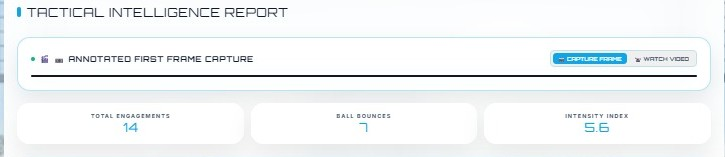
\includegraphics[width=0.90\textwidth]{images_chap3/statistic_A.jpeg}
  \caption{Bloc A — KPIs globaux du match}
  \label{fig:blockA}
\end{figure}

\subsubsection*{Bloc B — Tableau de score}
 
Affichage du score en temps réel entre \textbf{Team Gold} (Opérateurs 3 \& 4) et
\textbf{Team Blue} (Opérateurs 1 \& 2), avec un code couleur distinctif mis à jour
automatiquement par le module de détection de points.

\begin{figure}[H]
  \centering
  
\includegraphics[width=0.90\textwidth]{images_chap3/statistic_B.jpeg}
  \caption{Bloc B — Tableau de score}
  \label{fig:blockB}
\end{figure}

\subsubsection*{Bloc C — Cartes statistiques individuelles (4 joueurs)}
 
Chaque joueur est représenté par une carte statistique affichant neuf métriques biométriques
et tactiques :
 
\begin{table}[H]
  \centering
  \renewcommand{\arraystretch}{1.3}
  \begin{tabularx}{\textwidth}{L{3.2cm} X C{1.5cm}}
    \rowcolor{tablehead}
    \textcolor{white}{\textbf{Métrique}} &
    \textcolor{white}{\textbf{Description}} &
    \textcolor{white}{\textbf{Unité}} \\
    \rowcolor{rowalt}
    Points (PTS)      & Score total accumulé pendant le match & — \\
    Rating (\%)       & Note de performance globale normalisée sur 100 & \% \\
    \rowcolor{rowalt}
    Total Strikes     & Nombre total de frappes détectées & — \\
    Max Velocity      & Vitesse de déplacement maximale atteinte & km/h \\
    \rowcolor{rowalt}
    Distance Covered  & Distance totale parcourue sur l'ensemble du match & m \\
    Avg Tempo         & Vitesse de déplacement moyenne pendant les échanges & km/h \\
    \rowcolor{rowalt}
    Net Presence      & Taux de présence en zone de filet & \% \\
    Calories Burned   & Dépense énergétique estimée par intégration de la distance & kCal \\
    \rowcolor{rowalt}
    Overheads Ratio   & Ratio de frappes en hauteur sur le total des frappes & \% \\
  \end{tabularx}
  \caption{Métriques biométriques et tactiques par joueur}
  \label{tab:metriques_joueur}
\end{table}
 
Le joueur affichant le meilleur rating est mis en valeur visuellement par un badge
\textbf{"TOP"} coloré dans l'angle de sa carte. Dans l'exemple fourni, l'Opérateur 2
(Team Blue) se distingue avec \textbf{31 PTS} et un rating de tête, traduisant une
domination tactique et physique sur le match.
 
\begin{figure}[H]
  \centering
  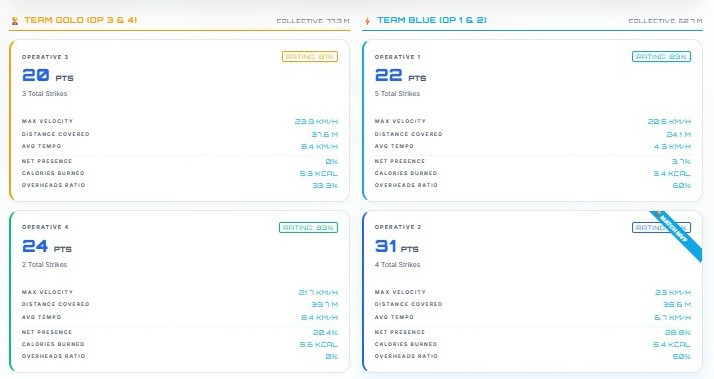
\includegraphics[width=0.90\textwidth]{images_chap3/statistic_C.jpeg}
  \caption{Bloc C — Cartes statistiques individuelles par joueur}
  \label{fig:blockC}
\end{figure}

\subsubsection*{Bloc D — Télémétrie de vitesse}
 
Graphique linéaire multi-courbes généré par Plotly.js, représentant la vitesse de
déplacement (km/h) de chacun des 4 joueurs en fonction du temps (identifiant de frame de
session). Chaque courbe est colorée distinctement selon l'opérateur (OP1, OP2, OP3, OP4).
Ce graphique interactif permet d'identifier :
 
\begin{itemize}[leftmargin=1.5em]
  \item Les pics d'effort correspondant aux sprints défensifs ou aux retours de balle
  \item Les phases de récupération visibles sous forme de plateaux à vitesse nulle ou faible
  \item Les asymétries d'effort entre partenaires d'une même équipe ou entre les deux équipes
\end{itemize}
 
\begin{figure}[H]
  \centering
  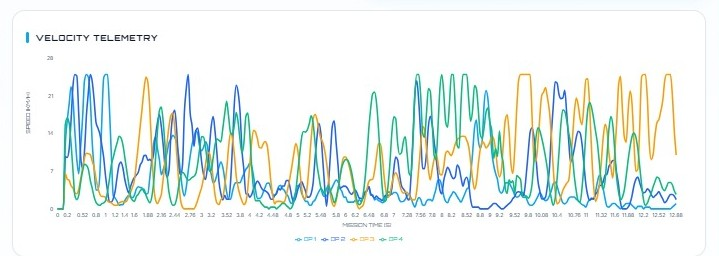
\includegraphics[width=0.90\textwidth]{images_chap3/statistic_D.jpeg}
  \caption{Bloc D — Graphique de télémétrie de vitesse}
  \label{fig:blockD}
\end{figure}

\subsubsection*{Bloc E — Strike Classification}
 
Répartition des types de frappes par joueur, affichée sous forme de badges colorés
comptabilisés pour chaque opérateur : SMASH, FOREHAND, BACKHAND, BANDEJA, LOB. Cette
classification croise la trajectoire de la balle et la posture du joueur au moment de
l'impact pour inférer automatiquement le type de frappe.

\begin{figure}[H]
  \centering
  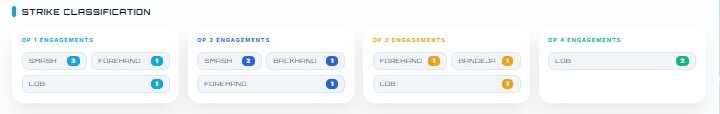
\includegraphics[width=0.90\textwidth]{images_chap3/statistic_E.jpeg}
  \caption{Bloc E — Classification des frappes}
  \label{fig:blockE}
\end{figure}
 
\subsubsection*{Bloc F — Historique des opérations (Recent Operations)}
 
Le bloc \textit{Opérations récentes} affiche les identifiants hexadécimaux des 7 dernières
analyses archivées (ex : \texttt{7C295C}, \texttt{B38164}...). Chaque identifiant correspond
à un fichier JSON stocké dans \texttt{/results\_json/}, permettant de recharger une analyse
passée sans relancer le traitement.
 
% ════════════════════════════════════════════════════════════════════════════
\section{Workflow utilisateur et exemples d'utilisation}
% ════════════════════════════════════════════════════════════════════════════
 
Le workflow complet d'un entraîneur utilisant SmartPlayAI se décompose en cinq étapes
successives :
 
% ─────────────────────────────────────────────────────────────────────────────
% FIGURE 4.5 — Workflow utilisateur
% Remplacez VOTRE_URL_IMAGE_4_5 par l'URL ou le chemin local de l'image
% ─────────────────────────────────────────────────────────────────────────────
\begin{figure}[H]
    \centering
    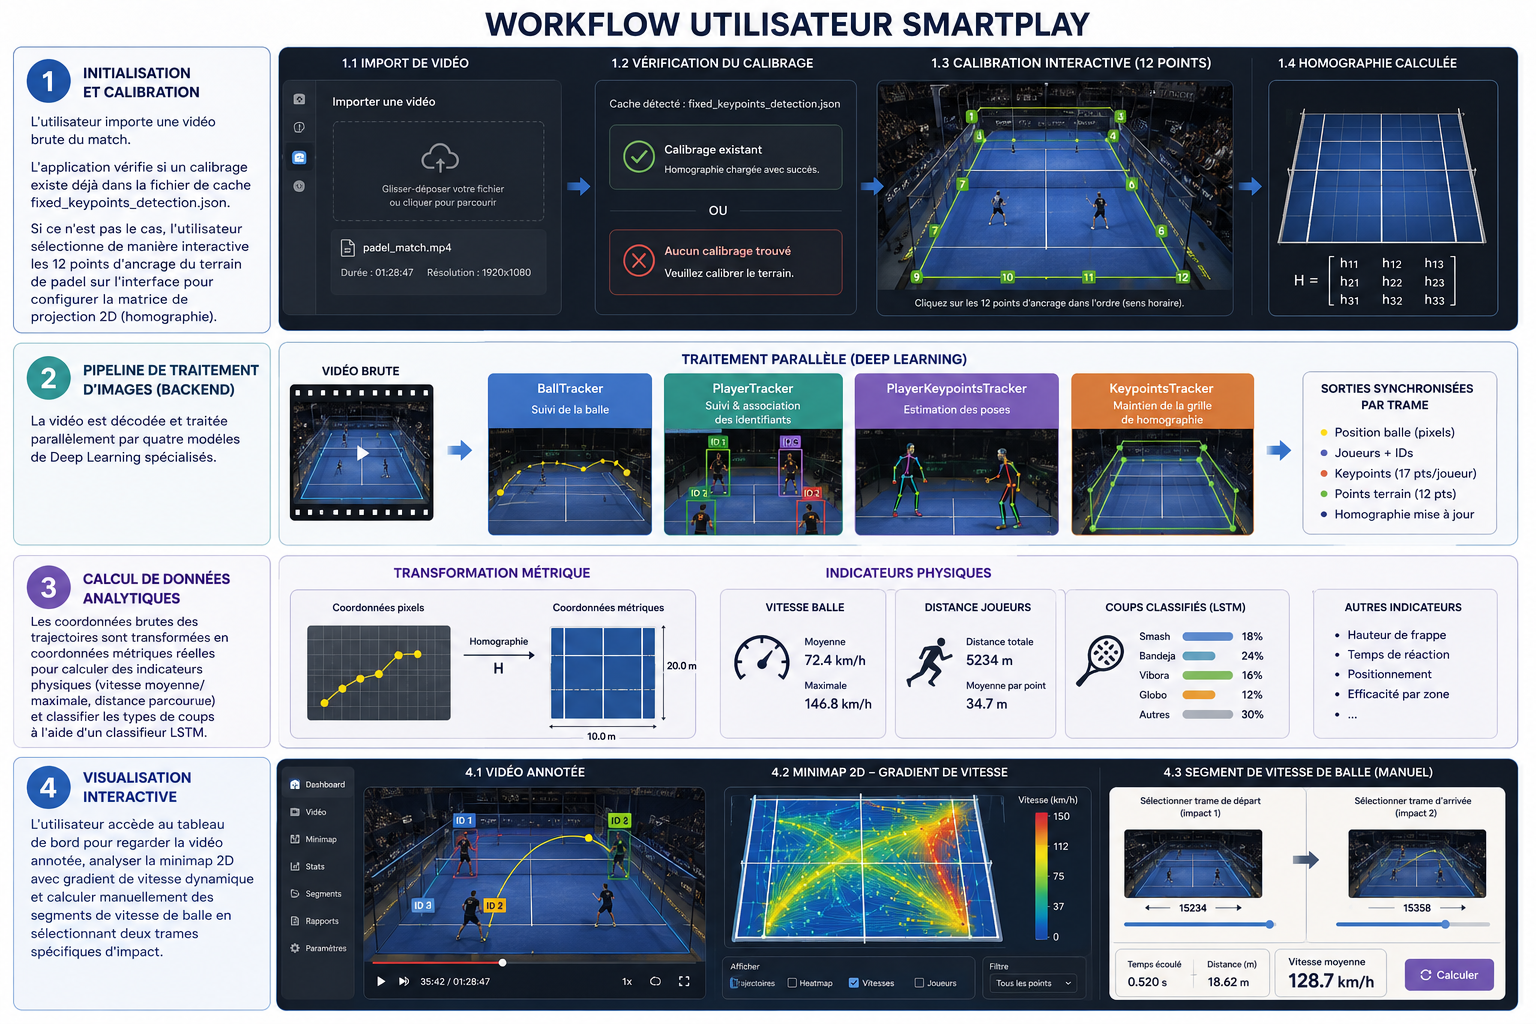
\includegraphics[width=0.90\textwidth]{images_chap3/place_holder.png}
    \caption{Workflow utilisateur complet d'une session d'analyse SmartPlayAI}
    \label{fig:workflow}
\end{figure}

\subsection*{Exemple d'utilisation 1 : analyse post-match d'un tournoi}
 
Un entraîneur reçoit la vidéo \texttt{.mp4} d'un match joué la veille lors d'un tournoi
régional. Il :
 
\begin{itemize}[leftmargin=1.5em]
  \item Importe la vidéo dans le panneau de configuration $\rightarrow$ l'interface confirme
        \textbf{VIDEO SYNCHRONIZED}
  \item Clique sur \textit{Capture Frame} $\rightarrow$ vérifie visuellement que le terrain
        est entièrement couvert
  \item Importe le fichier \texttt{court\_keypoints\_terrain\_A.json} (calibration
        préalablement effectuée pour ce terrain spécifique)
  \item Lance l'analyse via \textbf{LAUNCH NEURAL ANALYSIS} $\rightarrow$ observe le journal
        de mission pendant le traitement ($\sim$3--5 min)
  \item Consulte le rapport final : identifie que l'Opérateur 2 présente un ratio LOB de
        60\% et une vitesse maximale de 23 km/h, révélant une stratégie défensive dominante
\end{itemize}
 
\subsection*{Exemple d'utilisation 2 : suivi longitudinal d'un joueur}
 
L'entraîneur souhaite évaluer la progression d'un joueur sur plusieurs semaines. Il accède
à l'historique via le bloc \textit{Recent Operations} et charge successivement trois analyses
archivées (identifiées par leurs codes hexadécimaux \texttt{7C295C}, \texttt{B38164},
\texttt{C980BD}...) pour comparer l'évolution de la distance couverte, du tempo moyen et du
rating sur trois sessions consécutives.
 
\subsection*{Exemple d'utilisation 3 : calibration d'un nouveau terrain}
 
Pour un terrain n'ayant jamais été analysé, l'entraîneur utilise le champ
\textit{Advanced Parameters (JSON)} pour saisir manuellement les 12 keypoints identifiés
sur la frame capturée :
 
\begin{center}
\begin{lstlisting}[basicstyle=\small\ttfamily, backgroundcolor=\color{black!5},
                   frame=single]
[[145, 892], [1772, 887], [145, 695], [958, 695],
 [1772, 695], [145, 539], [1772, 539], [145, 384],
 [958, 384], [1772, 384], [145, 188], [1772, 183]]
\end{lstlisting}
\end{center}
 
Le système calcule la matrice d'homographie à partir de ces coordonnées et projette le
terrain sur un plan 2D normalisé aux dimensions réglementaires (10m × 20m), permettant
l'expression des métriques de distance et de vitesse en unités physiques réelles.
 
% ════════════════════════════════════════════════════════════════════════════
\section{Évaluation et validation de la solution}
% ════════════════════════════════════════════════════════════════════════════

Cette section a pour objectif d'évaluer la capacité de SmartPlayAI à répondre aux
exigences fonctionnelles et techniques définies au début du projet. L'évaluation
porte à la fois sur la validation des fonctionnalités offertes à l'utilisateur et
sur l'analyse des performances du pipeline d'intelligence artificielle dans
différentes conditions d'utilisation.

% ────────────────────────────────────────────────────────────────────────────
\subsection{Protocole de validation}
% ────────────────────────────────────────────────────────────────────────────

La validation de SmartPlayAI a été réalisée à travers une série de scénarios
représentatifs d'une utilisation réelle de la plateforme. Les tests ont porté sur
l'ensemble de la chaîne de traitement, depuis le chargement des vidéos jusqu'à la
génération des statistiques et des visualisations finales.

Les expérimentations ont été effectuées sur plusieurs vidéos de matchs de padel
enregistrées dans différentes conditions de résolution, d'éclairage et de qualité
d'acquisition. Les métriques observées concernent principalement la robustesse des
modules de détection, la cohérence des événements détectés ainsi que les
performances d'exécution du système.

% ────────────────────────────────────────────────────────────────────────────
\subsection{Validation fonctionnelle}
% ────────────────────────────────────────────────────────────────────────────

Les tests fonctionnels ont permis de vérifier le bon fonctionnement des
principales fonctionnalités développées au sein de SmartPlayAI. Les scénarios
évalués couvrent l'intégralité du \textit{workflow} applicatif : chargement et
lecture des vidéos, sélection des paramètres d'analyse, détection automatique des
joueurs, suivi de la balle, estimation des points clés corporels, génération des
statistiques biomécaniques, visualisation des résultats dans le tableau de bord et
exportation des données d'analyse.

Les résultats obtenus montrent que l'ensemble des fonctionnalités prévues dans le
cahier des charges a été implémenté et intégré avec succès dans une interface
unifiée.

% ────────────────────────────────────────────────────────────────────────────
\subsection{Évaluation des performances}
% ────────────────────────────────────────────────────────────────────────────

L'évaluation des performances a été conduite afin d'estimer les capacités du
système dans différentes configurations matérielles. Un \textit{benchmark} a été
réalisé sur la machine de développement, équipée uniquement d'un processeur
(sans GPU dédié), à l'aide des modèles utilisés en production : YOLO26 pour la
détection des joueurs (\texttt{imgsz=1280}), YOLOv8-Pose pour l'estimation de la
pose (\texttt{imgsz=1280}), un réseau léger pour la détection des points de repère
du terrain (\texttt{imgsz=640}), et TrackNet pour la détection de la balle
(entrée fixe $512 \times 288$).

Les mesures, consignées dans le tableau~\ref{tab:benchmark_cpu}, montrent que la
latence totale sur processeur seul dépasse deux secondes par image, quelle que
soit la résolution d'entrée. Ce résultat s'explique par le fait que les modèles
YOLO et TrackNet effectuent leurs inférences sur des tenseurs de taille fixe,
indépendamment de la résolution source. La résolution n'affecte donc que le coût
de décodage vidéo et de redimensionnement, qui demeure négligeable (moins de
vingt millisecondes même en 4K).

\begin{table}[H]
  \centering
  \renewcommand{\arraystretch}{1.3}
  \begin{tabularx}{\textwidth}{X C{2.2cm} C{2.2cm} C{2.2cm}}
    \rowcolor{tablehead}
    \textcolor{white}{\textbf{Module}} &
    \textcolor{white}{\textbf{720p (ms)}} &
    \textcolor{white}{\textbf{1080p (ms)}} &
    \textcolor{white}{\textbf{4K (ms)}} \\
    \rowcolor{rowalt}
    Décodage \& Redimensionnement & 2,2 & 3,8 & 16,3 \\
    Détection joueurs — YOLO26 (\texttt{imgsz=1280}) & 794,7 & 669,2 & 660,7 \\
    \rowcolor{rowalt}
    Estimation pose — YOLOv8-Pose (\texttt{imgsz=1280}) & 856,6 & 698,0 & 682,6 \\
    Détection terrain — YOLOv8 léger (\texttt{imgsz=640}) & 61,4 & 35,0 & 39,0 \\
    \rowcolor{rowalt}
    Détection balle — TrackNet ($512\times288$, fixe) & 747,1 & 723,5 & 701,6 \\
    \rowcolor{tablehead}
    \textcolor{white}{\textbf{Total pipeline / image}} &
    \textcolor{white}{\textbf{2\,461,9}} &
    \textcolor{white}{\textbf{2\,129,5}} &
    \textcolor{white}{\textbf{2\,100,3}} \\
    \rowcolor{tablehead}
    \textcolor{white}{\textbf{FPS équivalent (CPU)}} &
    \textcolor{white}{\textbf{0,4}} &
    \textcolor{white}{\textbf{0,5}} &
    \textcolor{white}{\textbf{0,5}} \\
  \end{tabularx}
  \caption{Latences mesurées sur CPU par module et par résolution d'entrée}
  \label{tab:benchmark_cpu}
\end{table}

L'utilisation d'un processeur graphique compatible CUDA améliore significativement
les performances et permet d'atteindre environ dix-huit images par seconde pour
des vidéos Full HD, rendant une analyse quasi temps réel envisageable pour un
déploiement opérationnel.

% ────────────────────────────────────────────────────────────────────────────
\subsection{Analyse des résultats}
% ────────────────────────────────────────────────────────────────────────────

L'analyse des expérimentations met en évidence la robustesse globale de
l'architecture proposée. La combinaison des modules de détection, de suivi et
d'analyse permet de produire automatiquement des statistiques cohérentes et
exploitables pour l'analyse des matchs de padel.

Les meilleurs résultats ont été obtenus avec des vidéos Full HD
($1920 \times 1080$ pixels) enregistrées à une cadence comprise entre 30 et
60 images par seconde. Le tableau~\ref{tab:resolution_impact} synthétise l'impact
de la résolution d'entrée sur la qualité de détection et formule les
recommandations opérationnelles correspondantes.

\begin{table}[H]
  \centering
  \renewcommand{\arraystretch}{1.3}
  \begin{tabularx}{\textwidth}{L{3.5cm} C{2.5cm} C{3.5cm} X}
    \rowcolor{tablehead}
    \textcolor{white}{\textbf{Résolution}} &
    \textcolor{white}{\textbf{FPS source}} &
    \textcolor{white}{\textbf{Qualité de détection}} &
    \textcolor{white}{\textbf{Recommandation}} \\
    \rowcolor{rowalt}
    480p ($854\times480$)    & 30    & Insuffisante & Non recommandé \\
    720p ($1280\times720$)   & 30    & Acceptable   & Minimum opérationnel \\
    \rowcolor{rowalt}
    1080p ($1920\times1080$) & 30–60 & Bonne        & Recommandé (\textit{sweet-spot}) \\
    4K ($3840\times2160$)    & 30–60 & Excellente   & Optimal si GPU $\geq$ 8\,Go VRAM \\
  \end{tabularx}
  \caption{Impact de la résolution vidéo d'entrée sur la qualité de détection}
  \label{tab:resolution_impact}
\end{table}

Cette configuration offre un compromis satisfaisant entre précision de détection
et coût de calcul. En deçà de 720p, la balle présente un diamètre apparent
inférieur à trois à cinq pixels, ce qui compromet la fiabilité de la détection
par TrackNet.

% ════════════════════════════════════════════════════════════════════════════
\section{Discussion et limites de la solution}
% ════════════════════════════════════════════════════════════════════════════

% ────────────────────────────────────────────────────────────────────────────
\subsection{Forces et contributions de SmartPlayAI}
% ────────────────────────────────────────────────────────────────────────────

SmartPlayAI présente plusieurs contributions originales par rapport aux solutions
existantes. Premièrement, la plateforme a été conçue spécifiquement pour le
padel, contrairement aux outils généralistes disponibles. Cette spécialisation a
permis d'intégrer des modèles et des traitements adaptés aux caractéristiques
particulières de ce sport, notamment la grande vitesse de déplacement de la balle
et la présence de surfaces vitrées réfléchissantes.

Deuxièmement, l'architecture modulaire facilite l'évolution future du système en
permettant le remplacement ou l'amélioration indépendante de chaque composant
— BallTracker, PlayersTracker, KeypointsTracker et DataAnalytics — sans remettre
en cause l'ensemble du pipeline.

Troisièmement, la plateforme automatise l'intégralité du processus d'analyse,
depuis la vidéo brute jusqu'à la production de statistiques biomécaniques et
d'indicateurs tactiques, sans nécessiter d'intervention manuelle entre les étapes.
Enfin, le recours à des inférences à taille fixe pour les modèles YOLO
(\texttt{imgsz=1280}) et TrackNet ($512\times288$) confère au système un coût de
traitement prévisible et indépendant de la résolution source, ce qui simplifie la
gestion des performances sur différentes configurations matérielles.

% ────────────────────────────────────────────────────────────────────────────
\subsection{Limites techniques identifiées}
% ────────────────────────────────────────────────────────────────────────────

Malgré les résultats obtenus, plusieurs limites subsistent. La détection de la
balle demeure sensible aux situations d'occlusion prolongée, aux réflexions sur
les surfaces vitrées du court ainsi qu'aux conditions d'éclairage défavorables. Si
le filtrage par marges géométriques réduit le nombre de faux positifs, il ne les
élimine pas entièrement lorsque la lumière rasante est particulièrement intense.

Par ailleurs, l'homographie est calculée une seule fois au démarrage du pipeline.
Tout mouvement de caméra au cours d'un enregistrement invalide la projection 2D et
nécessite une nouvelle calibration manuelle, ce qui constitue une contrainte
opérationnelle notable pour un déploiement sur le terrain.

Enfin, les performances du système diminuent lorsque la fréquence d'acquisition
est trop faible. TrackNet est optimisé pour une cadence de 25 à 30 images par
seconde ; en dessous de 15 FPS, les trajectoires deviennent discontinues et
l'interpolation parabolique génère des artefacts visibles sur les statistiques de
vitesse.

% ────────────────────────────────────────────────────────────────────────────
\subsection{Contraintes matérielles et opérationnelles}
% ────────────────────────────────────────────────────────────────────────────

L'exécution complète du pipeline nécessite des ressources matérielles importantes.
Le tableau~\ref{tab:hardware_requirements} présente les exigences minimales et
recommandées pour chaque composant du système, en distinguant le mode CPU seul
(traitement différé) du mode GPU CUDA (traitement quasi temps réel).

\begin{table}[H]
  \centering
  \renewcommand{\arraystretch}{1.3}
  \begin{tabularx}{\textwidth}{L{3.2cm} X X}
    \rowcolor{tablehead}
    \textcolor{white}{\textbf{Ressource}} &
    \textcolor{white}{\textbf{Minimum}} &
    \textcolor{white}{\textbf{Recommandé}} \\
    \rowcolor{rowalt}
    GPU VRAM          & 0 (CPU seul, $<$\,1\,FPS)    & 8\,Go (RTX\,3060, $\sim$18\,FPS) \\
    RAM système       & 16\,Go                        & 32\,Go \\
    \rowcolor{rowalt}
    Résolution vidéo  & 720p ($1280\times720$)        & 1080p ($1920\times1080$) \\
    Fréquence d'images & 25\,FPS                      & 30–60\,FPS \\
    \rowcolor{rowalt}
    Espace disque     & 10\,Go                        & 50\,Go (sorties annotées) \\
    Support CUDA      & Non requis (mode dégradé)     & CUDA\,11.8+ \\
  \end{tabularx}
  \caption{Exigences matérielles minimales et recommandées}
  \label{tab:hardware_requirements}
\end{table}

Sans GPU disposant d'un support CUDA, le pipeline dépasse deux secondes de
traitement par image, rendant toute analyse en quasi temps réel impossible. Pour
un déploiement opérationnel à une cadence supérieure ou égale à quinze images par
seconde, un GPU NVIDIA disposant d'au moins huit gigaoctets de mémoire vidéo est
indispensable. La comparaison détaillée des performances CPU et GPU est présentée
dans le tableau~\ref{tab:cpu_gpu_comparison}.

\begin{table}[H]
  \centering
  \renewcommand{\arraystretch}{1.3}
  \begin{tabularx}{\textwidth}{X C{2.5cm} C{2.8cm} C{2.5cm}}
    \rowcolor{tablehead}
    \textcolor{white}{\textbf{Module}} &
    \textcolor{white}{\textbf{CPU (ms)}} &
    \textcolor{white}{\textbf{GPU estimé (ms)}} &
    \textcolor{white}{\textbf{Accélération}} \\
    \rowcolor{rowalt}
    Détection joueurs — YOLO26        &  795  & $\sim$18 & $\times$44 \\
    Estimation pose — YOLOv8-Pose     &  857  & $\sim$22 & $\times$39 \\
    \rowcolor{rowalt}
    Détection terrain — YOLOv8 léger  &   61  & $\sim$5  & $\times$12 \\
    Détection balle — TrackNet (CNN)  &  747  & $\sim$8  & $\times$93 \\
    \rowcolor{tablehead}
    \textcolor{white}{\textbf{Total pipeline}} &
    \textcolor{white}{\textbf{2\,462}} &
    \textcolor{white}{\textbf{$\sim$55}} &
    \textcolor{white}{\textbf{$\times$45}} \\
    \rowcolor{tablehead}
    \textcolor{white}{\textbf{FPS effectif}} &
    \textcolor{white}{\textbf{0,4\,FPS}} &
    \textcolor{white}{\textbf{$\sim$18\,FPS}} &
    \textcolor{white}{\textbf{—}} \\
  \end{tabularx}
  \caption{Comparaison des temps d'inférence CPU versus GPU par module}
  \label{tab:cpu_gpu_comparison}
\end{table}

La qualité des résultats dépend également de la qualité des vidéos fournies en
entrée. Les conditions d'acquisition recommandées sont détaillées dans les
tableaux~\ref{tab:video_formats} et~\ref{tab:lighting_conditions}, portant
respectivement sur le format de fichier et les conditions de luminosité.

\begin{table}[H]
  \centering
  \renewcommand{\arraystretch}{1.3}
  \begin{tabularx}{\textwidth}{L{2.8cm} L{3cm} X L{3.5cm}}
    \rowcolor{tablehead}
    \textcolor{white}{\textbf{Container}} &
    \textcolor{white}{\textbf{Codec}} &
    \textcolor{white}{\textbf{Avantages}} &
    \textcolor{white}{\textbf{Sources typiques}} \\
    \rowcolor{rowalt}
    MP4 (\texttt{.mp4}) & H.264 (AVC)    & Large compatibilité, décodage rapide, bon ratio qualité/compression & Caméras grand public, smartphones, caméras IP \\
    MOV (\texttt{.mov}) & H.264 / ProRes & ProRes quasi-sans perte, idéal pour capture haute précision         & Caméras professionnelles (Blackmagic, Canon) \\
    \rowcolor{rowalt}
    AVI (\texttt{.avi}) & MJPEG / H.264  & Compression limitée — utile pour tester le pipeline sans artefacts  & Caméras de surveillance ou de laboratoire \\
  \end{tabularx}
  \caption{Formats vidéo supportés et recommandations d'acquisition}
  \label{tab:video_formats}
\end{table}

\begin{table}[H]
  \centering
  \renewcommand{\arraystretch}{1.3}
  \begin{tabularx}{\textwidth}{L{3.5cm} C{2.5cm} X L{4cm}}
    \rowcolor{tablehead}
    \textcolor{white}{\textbf{Situation}} &
    \textcolor{white}{\textbf{Luminosité (lux)}} &
    \textcolor{white}{\textbf{Effet sur le pipeline}} &
    \textcolor{white}{\textbf{Réglage recommandé}} \\
    \rowcolor{rowalt}
    Éclairage naturel doux (indoor)       & 300–500    & Bonne visibilité des lignes, balance de couleur neutre          & ISO 400–800, balance automatique \\
    Lumière forte / plein soleil (outdoor) & $>$\,1\,000 & Reflets et \textit{flare} $\rightarrow$ faux positifs de balle & Filtre polarisant, ISO 200–400, obturateur 1/1\,000\,s \\
    \rowcolor{rowalt}
    Éclairage faible / soirée (indoor)    & $<$\,200   & Bruit vidéo, perte de contraste, balle $<$ 3\,px               & ISO 800–1\,600, LED diffuse ($\sim$500\,lux), gamma $\approx$ 1,2 \\
    Éclairage directionnel / spot         & 500–800    & Ombres nettes perturbant la segmentation du fond                & Diffuseur, filtre médian $3\times3$ avant détection \\
  \end{tabularx}
  \caption{Conditions de luminosité et réglages recommandés pour l'acquisition}
  \label{tab:lighting_conditions}
\end{table}

% ────────────────────────────────────────────────────────────────────────────
\subsection{Perspectives d'amélioration}
% ────────────────────────────────────────────────────────────────────────────

Plusieurs pistes d'amélioration peuvent être envisagées pour renforcer les
capacités et élargir le champ d'application de SmartPlayAI.

Sur le plan de l'optimisation des performances, la conversion des modèles YOLO et
TrackNet au format TensorRT permettrait de réduire la latence GPU d'un facteur
deux à trois supplémentaires. La parallélisation de la détection des joueurs et de
la balle par traitement par lots (\textit{batching}) offrirait une meilleure
utilisation du processeur graphique et faciliterait l'atteinte des trente images
par seconde en continu.

Sur le plan fonctionnel, la suppression de l'étape manuelle de sélection des
points du terrain par une détection automatique des lignes — via un modèle
spécialisé — constituerait une amélioration significative de l'ergonomie de la
plateforme. L'intégration d'un réseau récurrent de type LSTM permettrait en outre
de prédire automatiquement le type de coup effectué (smash, lob, bandeja) à partir
des séquences de points clés corporels.

Sur le plan du déploiement, l'extension du pipeline à des configurations
multi-caméras améliorerait la couverture du terrain et réduirait les zones
d'occlusion. Le portage sur GPU embarqué de type NVIDIA Jetson ouvrirait enfin la
voie à une installation autonome directement sur le court, sans dépendance
vis-à-vis d'un serveur distant. À plus long terme, l'adaptation du système à
d'autres sports de raquette constitue une perspective d'extension naturelle de
l'architecture développée.

% ════════════════════════════════════════════════════════════════════════════
\section{Conclusion}
% ════════════════════════════════════════════════════════════════════════════
 
Ce chapitre a présenté en détail la réalisation de l'interface utilisateur SmartPlayAI, depuis
la définition des spécifications fonctionnelles jusqu'à l'implémentation et la description
des différentes vues de l'application.
 
L'interface se distingue par son approche holistique de l'analyse sportive : elle ne se
limite pas à afficher des statistiques brutes, mais propose un workflow guidé en cinq étapes
permettant à un entraîneur de padel, sans compétences techniques particulières, de piloter
un pipeline d'intelligence artificielle complet et d'en exploiter les résultats de manière
immédiate et lisible.
 
Le panneau de configuration — chargement vidéo, calibration terrain, déclenchement de
l'analyse — et le tableau de bord tactique — KPIs globaux, cartes joueurs, télémétrie
vitesse, classification des frappes — forment un système cohérent et complémentaire, conçu
pour répondre aux besoins réels des entraîneurs lors des phases d'analyse post-match et de
suivi longitudinal des performances.
 
Les choix technologiques retenus (React et Vite en frontend, FastAPI et Python en backend,
YOLO et TrackNet pour l'IA, déploiement via Docker) garantissent à la fois la réactivité de
l'interface, la puissance du traitement et la modularité du système, ouvrant la voie aux
évolutions et aux extensions décrites dans la conclusion générale du rapport.
 
\bigskip
\begin{center}
  \textit{— Fin du chapitre —}
\end{center}


% Include general conclusion
\cleardoublepage
% Conclusion Générale
\chapter*{Conclusion Générale}
\addcontentsline{toc}{chapter}{Conclusion Générale}

\section*{Synthèse des contributions}

Ce mémoire a présenté SmartPlay, une plateforme intelligente d'analyse vidéo automatisée dédiée au padel, développée dans le cadre d'un projet de fin d'études réalisé au sein de la startup tunisienne Ultima. L'objectif central était de concevoir un système capable d'analyser automatiquement des matchs de padel à partir de flux vidéo bruts, en extrayant des métriques tactiques et biométriques précises, sans aucune intervention humaine.

\section*{Apports techniques et architecturaux}

Sur le plan technique, la solution repose sur une architecture modulaire en pipeline combinant plusieurs technologies de pointe. Le module de détection du terrain, basé sur YOLOv8-Pose, établit le socle géométrique du système en localisant douze points de référence et en calculant la matrice d'homographie permettant une projection métrique précise. Le module de suivi de la balle, fondé sur TrackNet et enrichi d'une chaîne de post-traitement physiquement informée, atteint un taux de détection correct de 96,2 \% (PCK@5px), contre 86,5 \% pour le modèle brut, démontrant l'apport significatif des filtres cinématiques et de l'interpolation parabolique. Le module de suivi des joueurs garantit des identifiants stables sur toute la durée du match grâce à l'algorithme Hongrois et à un mécanisme de persistance prédictive allant jusqu'à 90 trames. Enfin, le module DataAnalytics construit un DataFrame cinématique de 179 colonnes regroupant déplacements, vitesses, accélérations et événements de jeu, alimentant directement le tableau de bord tactique de l'interface utilisateur.

\section*{Apports fonctionnels et accessibilité}

Sur le plan fonctionnel, l'interface SmartPlay, développée avec React et FastAPI, propose un workflow guidé en cinq étapes permettant à un entraîneur ou un analyste sportif — sans compétences techniques particulières — de piloter un pipeline d'intelligence artificielle complet. Le tableau de bord tactique restitue en temps réel les KPIs globaux du match, les statistiques individuelles de chaque joueur, la télémétrie de vitesse et la classification des frappes par type (smash, bandeja, forehand, backhand, volley, service). L'architecture basée sur Docker garantit un déploiement sans infrastructure lourde, démocratisant ainsi l'accès à des outils d'analyse jusqu'alors réservés aux structures professionnelles.

\section*{Positionnement concurrentiel}

En termes de positionnement, SmartPlay se distingue des solutions existantes (Padelytics, Hudl, Dartfish) par trois avantages structurels : une spécialisation disciplinaire complète pour le padel, une accessibilité aux structures amateurs grâce à un déploiement sans infrastructure lourde, et un moteur de scoring automatique basé sur une machine à états finis conforme aux règles officielles du padel.

\section*{Limites et opportunités d'amélioration}

Cependant, ce travail présente certaines limites qu'il convient de reconnaître. Le système a été évalué sur un ensemble de séquences vidéo limité, et ses performances dans des conditions d'éclairage extrêmes ou avec des caméras de très faible résolution restent à valider. La classification des coups, bien qu'opérationnelle, bénéficierait d'un jeu de données d'entraînement plus large pour améliorer sa précision sur les types de frappes rares. De plus, l'approche mono-caméra actuelle, bien que fonctionnelle, ne permet pas de capturer la complexité tridimensionnelle entière des trajectoires balistiques.

\section*{Perspectives et axes d'évolution}

En perspectives, plusieurs axes d'évolution majeurs sont envisagés pour les prochaines itérations de la plateforme :

\subsection*{Court terme : Consolidation et robustesse}

\begin{itemize}
    \item \textbf{Amélioration du module de détection de fond :} mieux distinguer la balle des distractions visuelles telles que les spectateurs, les panneaux publicitaires ou les éléments de clôture, particulièrement dans les environnements d'entraînement peu structurés.
    \item \textbf{Enrichissement du jeu de données de classification :} collecte systématique de milliers de coups annotés manuellement pour améliorer la précision de la reconnaissance des types de frappes rares (contre-bande, vibora, etc.).
    \item \textbf{Optimisation des performances computationnelles :} réduction de la latence de traitement pour approcher l'analyse temps réel avec des débits vidéo standards (25-30 FPS).
\end{itemize}

\subsection*{Moyen terme : Évolution technologique}

\begin{itemize}
    \item \textbf{Reconstruction 3D de la trajectoire de la balle :} passage à une approche multi-caméra calibrée permettant une analyse fine de la hauteur, de la vitesse angulaire et de l'effet de rotation indépendamment de la perspective. Cette évolution constituerait un saut qualitatif majeur pour l'analyse biomécanique et tactique.
    \item \textbf{Analyse temps réel en compétition :} déploiement d'une version cloud capable de traiter les flux vidéo en direct lors des matchs officiels, avec transmission en flux continu des statistiques vers les entraîneurs sur tablette et génération de rapports live.
    \item \textbf{Module d'intelligence tactique autonome :} intégration d'un système de recommandations personnalisées fondé sur des modèles d'apprentissage automatique, exploitant l'historique des sessions de chaque joueur pour suggérer des ajustements stratégiques basés sur les patterns adverses détectés.
\end{itemize}

\subsection*{Long terme : Expansion écosystémique}

\begin{itemize}
    \item \textbf{Extension multi-sports :} adaptation du système vers d'autres sports de raquette tels que le tennis et le squash, en généralisant les modèles de détection et en adaptant les règles de l'automate de scoring. Cette approche modulaire réutiliserait l'architecture core tout en adaptant les briques métier.
    \item \textbf{Application mobile native :} développement d'une application iOS/Android offrant une interface tactile optimisée pour la consultation des analyses en temps réel, avec synchronisation cloud et partage de vidéos annotées entre entraîneurs et joueurs.
    \item \textbf{Intégration avec des capteurs biométriques portables :} fusion des données vidéo avec des flux de fréquence cardiaque, d'accélération inertielle et d'oxymétrie pour une analyse holistique de la performance physique et cognitive.
    \item \textbf{Plateforme collaborative cloud :} création d'un écosystème centralisé permettant aux clubs, entraîneurs et joueurs de partager des analyses, de comparer des performances entre structures et de contribuer collectivement à l'amélioration des modèles d'IA.
\end{itemize}

\section*{Impact et contribution à l'écosystème du padel}

En définitive, SmartPlay constitue une contribution concrète à la démocratisation de l'analyse sportive de haute performance. En transformant un simple flux vidéo en données analytiques structurées et exploitables, la plateforme ouvre la voie à une nouvelle génération d'outils de coaching intelligents, accessibles non seulement aux clubs professionnels, mais également aux structures amateurs qui constituent l'immense majorité des pratiquants de padel dans le monde.

Cette démocratisation revêt une importance particulière dans un contexte où le padel connaît une croissance exponentielle au niveau international. L'accès à des outils d'analyse de qualité professionnelle, jusqu'à présent limité aux structures bien financées, peut significativement élever le niveau moyen de coaching dans les clubs régionaux et locaux, contribuant ainsi à la professionnalisation progressive de la discipline.

Au-delà du padel, SmartPlay démontre la viabilité d'une approche générique pour l'analyse vidéo intelligente de sports collectifs ou individuels. L'architecture modulaire et les briques technologiques développées (détection géométrique, suivi multi-cible, extraction de métriques biométriques) constituent une base réutilisable pour de futurs projets dans d'autres domaines sportifs, ou même au-delà du sport dans des applications de surveillance, d'analyse comportementale ou de métrologie vidéo.

Enfin, cette démarche illustre comment une startup tunisienne peut créer de la valeur en appliquant les techniques les plus récentes de l'intelligence artificielle et du computer vision à un domaine spécialisé, générant ainsi des solutions compétitives sur le marché international tout en répondant aux besoins spécifiques d'une communauté sportive en croissance rapide.


% ------------------ Bibliography ------------------
\cleardoublepage
\phantomsection
\addcontentsline{toc}{chapter}{Références}
% Si vous utilisez biblatex, assurez-vous que le fichier `references.bib` existe.
\printbibliography[title=Références]

\renewcommand{\thechapter}{\arabic{chapter}}

\end{document}
